% Task C05
% Source volume: upper
% Physical scan pages: 141--173
% Printed book pages: 124--156
% Transcribe only source content; omit running headers, footers, and printed page numbers.
\chapter{连续函数}

% BEGIN TRANSCRIPTION

连续函数类是数学分析中的主要函数类之一。有关连续函数的一系列重要结论是支持数学分析整个体系的支柱。本章的主要内容是介绍连续函数的基本定理。由于这些性质都和连续函数的整个定义域密切联系，与局部有界性、局部保号性等局部性质有根本的不同，因此称为连续函数的整体性质，或非局部性质。

在 §5.1 的基本概念之后，将基本定理分成三组，逐节介绍它们的方法和应用。§5.5 为单调函数。在 §5.6 中介绍连续函数在混沌中的应用，这是 §2.6（迭代生成数列）的现代发展。最后一节为学习要点和两组参考题。

\section{连续性概念}

\subsection{内容提要}

\begin{enumerate}
  \item 函数 $f$ 在点 $a$ 连续有两个定义：(1) 第一定义是：$\lim_{x\to a}f(x)=f(a)$；(2) 第二定义是：对于收敛于 $a$ 的每个数列 $\{x_n\}$，有 $\lim_{n\to\infty}f(x_n)=f(a)$。两个定义的等价性可用函数极限的 Heine 归结原理得到。
  \item 函数 $f$ 在点 $a$ 左连续（右连续）的定义是：$f(a^-)=f(a)$（$f(a^+)=f(a)$）。函数 $f$ 在点 $a$ 连续的充分必要条件是 $f(a^-)=f(a)=f(a^+)$。
  \item 设点 $a$ 属于函数 $f$ 的定义域，若 $f$ 在 $a$ 连续，则称 $a$ 为 $f$ 的连续点，否则称点 $a$ 为函数 $f$ 的不连续点，即间断点。间断点的分类：若存在两个单侧极限，则为第一类，否则为第二类。（请注意：各种教材对于间断点的定义不完全相同。）
  \item 区间上连续函数的定义：函数 $f$ 在区间 $I$ 的每一点都连续（即处处连续），则称函数 $f$ 在区间 $I$ 上连续。若区间包含端点，则在端点处的连续性是按左连续或右连续来定义的。本书经常采用记号 $f\in C(I)$ 表示函数 $f$ 为区间 $I$ 上的连续函数。
  \item 用函数在一个点的振幅来刻画连续性有时是很方便的。其定义如下。对于点 $a$ 的邻域 $O_\delta(a)$，定义 $f$ 在这个邻域上的振幅为
  \[
    \omega_f(a,\delta)=\sup_{x\in O_\delta(a)}\{f(x)\}-\inf_{x\in O_\delta(a)}\{f(x)\},
  \]
  然后令
  \[
    \omega_f(a)=\lim_{\delta\to0^+}\omega_f(a,\delta),
  \]
  称为函数 $f$ 在点 $a$ 的振幅。容易证明，函数 $f$ 在点 $a$ 连续的充分必要条件是 $\omega_f(a)=0$（留作为 5.1.4 小节的练习题 12）。
\end{enumerate}

\subsection{思考题}

\begin{xthought}[1]
当 $f$ 于点 $a$ 连续时，函数 $f^2$ 和 $|f|$ 在点 $a$ 是否连续？反之如何？
\end{xthought}
\begin{xsolution}
若 $f$ 在 $a$ 连续，则由连续函数的四则运算以及绝对值函数的连续性，$f^2$ 与 $|f|$ 都在 $a$ 连续。

反之均不成立。例如令
\[
 f(x)=\begin{cases}
  1,&x\ge a,\\
  -1,&x<a.
 \end{cases}
\]
则 $f$ 在 $a$ 不连续，而 $f^2\equiv1$、$|f|\equiv1$ 均在 $a$ 连续。因此仅由 $f^2$ 或 $|f|$ 在 $a$ 连续不能推出 $f$ 在 $a$ 连续。
\end{xsolution}


\begin{xthought}[2]
设函数 $f,g$ 在点 $a$ 都不连续，问 $f+g$ 和 $f\cdot g$ 在点 $a$ 是否连续？
\end{xthought}
\begin{xsolution}
不能由“$f,g$ 在 $a$ 都不连续”唯一判断 $f+g$ 或 $fg$ 是否连续。

例如取 Dirichlet 函数 $D$，令 $f=D,g=1-D$，则 $f,g$ 处处不连续，但
\[
 f+g\equiv1,\qquad fg\equiv0
\]
处处连续。另一方面，若取 $f=g=D$，则 $f+g=2D$、$fg=D$ 都处处不连续。因此和与积既可能连续，也可能不连续。
\end{xsolution}


\begin{xthought}[3]
设函数 $f$ 在区间 $(a,b)$ 上定义，若对于每个闭区间 $[c,d]\subset(a,b)$，函数 $f$ 在 $[c,d]$ 上连续，证明 $f$ 在 $(a,b)$ 上连续。
\end{xthought}
\begin{xsolution}
任取 $x_0\in(a,b)$。可取 $c,d$ 使
\[
 a<c<x_0<d<b.
\]
由题设，$f$ 在闭区间 $[c,d]$ 上连续，特别地在其内点 $x_0$ 连续。由于 $x_0$ 任意，$f$ 在 $(a,b)$ 上处处连续，即 $f\in C(a,b)$。
\end{xsolution}


\begin{xthought}[4]
讨论下列函数的连续性，若有间断点则确定它的类型：
  \begin{enumerate}[label=(\arabic*)]
    \item $f(x)=\begin{cases}\ee^{1/x},&x\in(-\infty,0),\\x^2,&x\in[0,+\infty);\end{cases}$
    \item $f(x)=\begin{cases}\ee^{1/x},&x\in\RR-\{0\},\\0,&x=0;\end{cases}$
    \item $f(x)=\begin{cases}\dfrac{\ln(1+x^2)}{x},&x\in(-1,0)\cup(0,1),\\2,&x=0.\end{cases}$
  \end{enumerate}
\end{xthought}
\begin{xsolution}
\begin{enumerate}[label=(\arabic*)]
 \item 当 $x\to0^-$ 时，$1/x\to-\infty$，故 $\ee^{1/x}\to0$；当 $x\to0^+$ 时，$x^2\to0$，且 $f(0)=0$。所以 $f$ 在 $0$ 连续。其余各点由初等函数连续性知均连续。因此 $f$ 在 $\RR$ 上连续。
 \item 除 $0$ 外均连续。在 $0$ 处
 \[
  \lim_{x\to0^-}\ee^{1/x}=0,\qquad
  \lim_{x\to0^+}\ee^{1/x}=+\infty,
 \]
 两个单侧极限不能同时作为有限实数存在，故 $0$ 为第二类间断点。
 \item 对 $x\ne0$，
 \[
  \frac{\ln(1+x^2)}x
  =x\,\frac{\ln(1+x^2)}{x^2}\longrightarrow0
  \qquad(x\to0),
 \]
 因为 $\ln(1+u)/u\to1$。而 $f(0)=2$，所以 $0$ 为可去间断点；在 $(-1,0)\cup(0,1)$ 上函数连续。
\end{enumerate}
\end{xsolution}


\begin{xthought}[5]
找出下列函数的间断点，并确定类型：
  \begin{enumerate}[label=(\arabic*)]
    \item $f(x)=\operatorname{sgn}x$；
    \item $g(x)=x-[x]$；
    \item $f(g(x))$（$f$ 和 $g$ 由 (1),(2) 给定）；
    \item $g(f(x))$（$f$ 和 $g$ 同 (3)）；
    \item $h(x)=\dfrac{\dfrac1x-\dfrac1{x+1}}{\dfrac1{x-1}-\dfrac1x}$；
    \item $y(x)=\dfrac{1}{\left[\dfrac1x\right]}$。
  \end{enumerate}
\end{xthought}
\begin{xsolution}
\begin{enumerate}[label=(\arabic*)]
 \item $\operatorname{sgn}x$ 只在 $x=0$ 间断，且
 \[
  f(0^-)=-1,\qquad f(0^+)=1,
 \]
 故 $0$ 为跳跃间断点。

 \item $g(x)=x-[x]$ 为小数部分函数。对每个 $m\in\ZZ$，
 \[
  g(m^-)=1,\qquad g(m^+)=g(m)=0,
 \]
 故所有整数都是跳跃间断点；其余点连续。

 \item 由 $g(x)\in[0,1)$，且 $g(x)=0$ 当且仅当 $x\in\ZZ$，有
 \[
  f(g(x))=\begin{cases}0,&x\in\ZZ,\\1,&x\notin\ZZ.
  \end{cases}
 \]
 对任意整数 $m$，$\lim_{x\to m}f(g(x))=1$ 而函数值为 $0$，故每个整数都是可去间断点；其余点连续。

 \item 因为 $f(x)\in\{-1,0,1\}\subset\ZZ$，而 $g(k)=0$ 对每个整数 $k$ 成立，所以
 \[
  g(f(x))\equiv0,
 \]
 因而处处连续。

 \item 原式定义域排除 $x=-1,0,1$。在定义域内可化为
 \[
  h(x)=\frac{x-1}{x+1}.
 \]
 因此 $x=0,1$ 均为可去间断点；在 $x=-1$ 处函数无界，故为第二类间断点。

 \item 定义域为
 \[
  (-\infty,0)\cup(0,1],
 \]
 因为当 $x>1$ 时 $[1/x]=0$。在每个使 $1/x$ 不越过整数的开区间内函数为常数。对 $n\in\NN_+$，点 $x=-1/n$ 的左右函数值分别趋于 $-1/n$ 与 $-1/(n+1)$，故都是跳跃点；对 $n\ge2$，点 $x=1/n$ 的左右函数值分别为 $1/n$ 与 $1/(n-1)$，故也是跳跃点。点 $x=1$ 按定义域的左侧连续。因此全部间断点为
 \[
  \left\{-\frac1n:n\in\NN_+\right\}
  \cup
  \left\{\frac1n:n\ge2\right\},
 \]
 且均为跳跃间断点。
\end{enumerate}
\end{xsolution}


\subsection{例题}

\begin{xexample}[5.1.1]
设函数 $f$ 在 $x=0$ 处连续，对每一个 $x\in\RR$ 成立 $f(x)=f(2x)$。证明：$f$ 是常值函数。
\end{xexample}
\begin{xproof}
任取一个 $x\in\RR$，则
\[
  f(x)=f\left(2\cdot\frac{x}{2}\right)=f\left(\frac{x}{2}\right)=f\left(\frac{x}{2^2}\right)=\cdots=f\left(\frac{x}{2^n}\right).
\]
利用 $f(x)$ 在 $x=0$ 连续，因此（根据连续性的第二定义）
\[
  \lim_{n\to\infty}f\left(\frac{x}{2^n}\right)=f(0).
\]
这样就知道对每一个 $x\in\RR$ 成立 $f(x)=f(0)$。
\end{xproof}

\begin{xexample}[5.1.2]
设函数 $f,g$ 是 $(-\infty,+\infty)$ 上的连续函数，又在所有有理点上 $f(x)=g(x)$，证明：$f(x)\equiv g(x)$。
\end{xexample}
\begin{xproof}
只要对 $\RR$ 中的每个无理数 $x$ 证明 $f(x)=g(x)$ 成立即可。取有理数列 $\{r_n\}$，使 $\lim_{n\to\infty}r_n=x$。例如，取无理数 $x$ 的不足近似值 $r_n=[10^n x]/10^n$，则有
\[
  r_n=\frac{[10^n x]}{10^n}=\frac{10^n x-\theta_{x,n}}{10^n},
\]
其中 $0\le \theta_{x,n}<1$。因此就有 $r_n\to x\ (n\to\infty)$。

由于 $f(r_n)=g(r_n),n\in\NN_+$，$f,g$ 在点 $x$ 连续，利用连续性的第二定义，就有
\[
  f(x)=\lim_{n\to\infty}f(r_n)=\lim_{n\to\infty}g(r_n)=g(x).
\]
\end{xproof}

\begin{xexample}[5.1.3（一个函数方程的连续解）]
设函数 $f$ 在 $x=0$ 处连续，且对一切 $x,y$ 有 $f(x+y)=f(x)+f(y)$。证明 $f$ 在 $\RR$ 上连续，且 $f(x)=f(1)x$。
\end{xexample}
\begin{xproof}
在方程 $f(x+y)=f(x)+f(y)$ 中令 $y=0$，可知 $f(0)=0$。因此有
\[
  \lim_{x\to0}f(x)=0.
\]
任取点 $x_0\in\RR$，将 $x$ 写成 $x=x_0+\Delta x$，计算极限
\[
\begin{aligned}
  \lim_{x\to x_0}f(x)
  &=\lim_{\Delta x\to0}f(x_0+\Delta x)\\
  &=\lim_{\Delta x\to0}[f(x_0)+f(\Delta x)]\\
  &=f(x_0)+\lim_{\Delta x\to0}f(\Delta x)=f(x_0),
\end{aligned}
\]
可见 $f$ 处处连续。

由于 $f(x)+f(-x)=f(x+(-x))=f(0)=0$，可见有 $f(-x)=-f(x)$。因此只需讨论 $x$ 为正数的情况。对正有理数 $x=m/n$，其中 $m,n\in\NN_+$，用数学归纳法可以知道对正整数 $m\in\NN_+$，成立
\[
  f(mx)=mf(x).
\]
再从
\[
  f(x)=f\left(n\cdot\frac{x}{n}\right)=nf\left(\frac{x}{n}\right)
\]
得到 $f(x/n)=\frac1n f(x)$。因此就有
\[
  f\left(\frac{m}{n}x\right)=mf\left(\frac{x}{n}\right)=\frac{m}{n}f(x).
\]
令 $x=1$，代入得到
\[
  f\left(\frac{m}{n}\right)=\frac{m}{n}f(1).
\]
因此，等式 $f(x)=f(1)x$ 对一切有理数 $x\in\QQ$ 已成立。最后，利用例题 5.1.2 的结论，就知道 $f(x)=f(1)x$ 对一切实数 $x$ 成立。
\end{xproof}

\begin{xremark}
本例与例题 5.1.1 都是函数方程问题（参见 [14, 44]）。但本例的结论和证明的方法具有较大的典型意义。函数方程方面的基本材料可以看 [59] 第一册的 §1.10。在 [66] 的第 48--50 页有这方面的较新材料。此外，本题所求出的是该函数方程的连续解。实际上，这个函数方程还有不连续解。由以上证明可见，这个方程的解只要在一个点上连续，就处处连续。因此所谓的不连续解一定是处处不连续的函数。有兴趣的读者可以参考 [58] 的第 68--70 页。
\end{xremark}

\begin{xexample}[5.1.4（Riemann（黎曼）函数的连续性）]
Riemann 函数的定义为
\[
  R(x)=\begin{cases}
    \dfrac1q,&x=\dfrac pq,\text{其中 }p,q\text{ 为互素整数},\ q>0,\\
    0,&x\text{ 为无理数}.
  \end{cases}
\]
确定 $R$ 的间断点及其类型。（对于 $x=0$，可写出 $0=0/1$，因此取 $R(0)=1$。）
\end{xexample}
\begin{xsolution}
以下主要是证明对每个 $x_0\in\RR$ 成立
\begin{equation}
  \lim_{x\to x_0}R(x)=0.
  \tag{5.1}
  \label{eq:5.1}
\end{equation}
如果这一点已得到证明，则从函数 $R(x)$ 的定义即可以知道，在所有无理点处 $R(x)$ 连续，而在所有有理点处 $R(x)$ 不连续，且为可去间断点。

取定 $x_0$。由于 (5.1) 与 $R(x_0)$ 无关，因此无需区分 $x_0$ 是有理点或无理点。对给定的 $\varepsilon>0$，我们只需要证明有 $\delta>0$，使得当 $0<|x-x_0|<\delta$ 时，成立 $0\le R(x)<\varepsilon$。考虑其反面，使这个不等式不成立（即 $R(x)\ge\varepsilon$）的 $x$ 是什么？当然 $x$ 只能是有理数。将它写成 $x=p/q$，其中 $p,q$ 为互素的整数，$q>0$，则有
\[
  R\left(\frac pq\right)=\frac1q\ge\varepsilon.
\]
这等价于 $q\le1/\varepsilon$，即
\[
  q\in\left\{1,2,\ldots,\left[\frac1\varepsilon\right]\right\}.
\]
由以上分析可见，可以先取 $\delta_1=1$，然后将去心邻域
\[
  (x_0-1,x_0)\cup(x_0,x_0+1)
\]
% SOURCE-ERR: 原书此处将去心邻域印作 (x_0-1)\cup(x_0+1)；由“去心邻域”及上下文可确定为上述两开区间之并。
中分母为 $q\in\{1,2,\ldots,[1/\varepsilon]\}$ 的所有有理数 $p/q$ 都挑出来。由于这样的有理数至多只有有限个，可以将它们记为 $x_1,x_2,\ldots,x_k$，然后取
\[
  \delta=\min\{1,|x_1-x_0|,|x_2-x_0|,\ldots,|x_k-x_0|\},
\]
则当 $0<|x-x_0|<\delta$ 时就成立 $0\le R(x)<\varepsilon$。因此 (5.1) 成立。
\end{xsolution}

\begin{xremark}
如果用 $\delta_1=\varepsilon^2/2$ 代替 $\delta_1=1$，则可以证明：在 $(x_0-\delta_1)\cup(x_0+\delta_1)$ 中分母 $q\le1/\varepsilon$ 的有理数 $p/q$ 至多只有一个（见 [42]）。
\end{xremark}

\subsection{练习题}

\begin{xexercise}[1]
\begin{enumerate}[label=(\arabic*)]
    \item 将对偶法则用于连续性的第一定义和第二定义，写出函数 $f$ 在点 $a$ 处不连续的两个正面叙述；
    \item 证明连续性的两个定义的等价性。
  \end{enumerate}
\end{xexercise}
\begin{xsolution}
\begin{enumerate}[label=(\arabic*)]
 \item 连续性第一定义的否定可写成：存在 $\varepsilon_0>0$，使对每个 $\delta>0$，总存在定义域中的 $x$ 满足
 \[
  0<|x-a|<\delta,\qquad |f(x)-f(a)|\ge\varepsilon_0.
 \]
 连续性第二定义的否定可写成：存在数列 $\{x_n\}$，$x_n\to a$，但 $f(x_n)\not\to f(a)$。等价地，可在取子列后写成存在 $\varepsilon_0>0$ 及 $x_n\to a$，使
 \[
  |f(x_n)-f(a)|\ge\varepsilon_0,\qquad n\in\NN_+.
 \]

 \item 先设第一定义成立。若 $x_n\to a$，则对任意 $\varepsilon>0$，由连续性可取 $\delta>0$，使 $|x-a|<\delta$ 时 $|f(x)-f(a)|<\varepsilon$。当 $n$ 充分大时 $|x_n-a|<\delta$，故 $|f(x_n)-f(a)|<\varepsilon$，于是 $f(x_n)\to f(a)$。

 反过来，若第一定义不成立，则由 (1) 存在 $\varepsilon_0>0$，对每个 $n$ 可取 $x_n$ 使
 \[
  0<|x_n-a|<\frac1n,
  \qquad |f(x_n)-f(a)|\ge\varepsilon_0.
 \]
 于是 $x_n\to a$，但 $f(x_n)\not\to f(a)$，与第二定义矛盾。因此两定义等价。
\end{enumerate}
\end{xsolution}


\begin{xexercise}[2]
讨论下述函数的间断点及其类型：
  \begin{enumerate}[label=(\arabic*)]
    \item $f(x)=[x]$；
    \item $f(x)=\begin{cases}\dfrac{\ee^{\sin x}-1}{x},&x\in(-\infty,0)\cup(0,+\infty),\\1,&x=0;\end{cases}$
    \item $f(x)=[x]+[-x]$；
    \item $f(x)=\begin{cases}\dfrac{x^2-x}{|x|(x^2-1)},&x\ne0,\pm1,\\1,&x=0,\pm1.\end{cases}$
  \end{enumerate}
\end{xexercise}
\begin{xsolution}
\begin{enumerate}[label=(\arabic*)]
 \item $[x]$ 在每个非整数点连续；对 $m\in\ZZ$，有
 \[
  [x]_{x\to m^-}=m-1,\qquad [m]=[x]_{x\to m^+}=m,
 \]
 所以所有整数均为跳跃间断点。

 \item 当 $x\to0$ 时
 \[
  \frac{\ee^{\sin x}-1}{x}
  =\frac{\ee^{\sin x}-1}{\sin x}\frac{\sin x}{x}\longrightarrow1=f(0).
 \]
 其余点处由初等函数连续性可知连续，故该函数处处连续。

 \item 若 $x\notin\ZZ$，则 $[x]+[-x]=-1$；若 $x\in\ZZ$，则该值为 $0$。所以每个整数处的极限均为 $-1$，函数值为 $0$，故所有整数都是可去间断点，其余点连续。

 \item 当 $x\ne0,\pm1$ 时
 \[
  \frac{x^2-x}{|x|(x^2-1)}
  =\frac{x}{|x|(x+1)}
  =\frac{\operatorname{sgn}x}{x+1}.
 \]
 因而在 $x=0$，左右极限分别为 $-1,1$，是跳跃点；在 $x=1$，极限为 $1/2$ 而函数值为 $1$，是可去间断点；在 $x=-1$，两侧分别无界，是第二类间断点。
\end{enumerate}
\end{xsolution}


\begin{xexercise}[3]
设函数 $f\in C[a,b]$。若有数列 $\{x_n\}\subset[a,b]$，使得 $\lim_{n\to\infty}f(x_n)=A$，证明：存在 $\xi\in[a,b]$，使得 $f(\xi)=A$。
\end{xexercise}
\begin{xsolution}
数列 $\{x_n\}\subset[a,b]$ 有收敛子列 $x_{n_k}\to\xi\in[a,b]$。由 $f$ 在 $\xi$ 连续，
\[
 f(x_{n_k})\to f(\xi).
\]
另一方面原数列满足 $f(x_n)\to A$，故其任意子列也趋于 $A$。由极限唯一性，$f(\xi)=A$。
\end{xsolution}


\begin{xexercise}[4]
设函数 $f$ 在 $(-\infty,+\infty)$ 上定义，在 $x=0,1$ 两点连续，且满足 $f(x)=f(x^2),x\in\RR$。证明：$f$ 是常值函数。
\end{xexercise}
\begin{xsolution}
若 $0<x<1$，则反复使用 $f(x)=f(x^2)$ 得
\[
 f(x)=f(x^{2^n}),
\]
而 $x^{2^n}\to0$，由 $f$ 在 $0$ 连续知 $f(x)=f(0)$。

若 $x>1$，令 $y_n=x^{1/2^n}$。由 $f(y)=f(y^2)$ 逐次反推得 $f(x)=f(y_n)$，而 $y_n\to1$，故由 $f$ 在 $1$ 连续，$f(x)=f(1)$。

又令 $x\to1^-$，前一结论给出 $f(x)=f(0)$，连续性于是推出 $f(1)=f(0)$。最后，对 $x<0$，有 $x^2>0$，故
\[
 f(x)=f(x^2)=f(0).
\]
所以 $f$ 在 $\RR$ 上为常值函数。
\end{xsolution}


\begin{xexercise}[5]
设在区间 $I$ 上函数 $f,g$ 连续，证明：$\max\{f,g\},\min\{f,g\}\in C(I)$。

  （可以从连续定义证，也可用公式 $\max\{a,b\}=\dfrac{a+b}{2}+\dfrac{|a-b|}{2}$ 等。）
\end{xexercise}
\begin{xsolution}
利用恒等式
\[
 \max\{f,g\}=\frac{f+g+|f-g|}{2},
 \qquad
 \min\{f,g\}=\frac{f+g-|f-g|}{2}.
\]
因为 $f,g$ 连续，所以 $f\pm g$ 连续，进而 $|f-g|$ 连续。因此上面两个函数均连续，即属于 $C(I)$。
\end{xsolution}


\begin{xexercise}[6]
设有三个函数 $f_1,f_2,f_3\in C[a,b]$，对每个 $x\in[a,b]$，定义 $f(x)$ 是三个函数值 $f_1(x),f_2(x),f_3(x)$ 中处于中间的一个值，证明：$f\in C[a,b]$。
\end{xexercise}
\begin{xsolution}
记
\[
 M(x)=\max\{f_1(x),f_2(x),f_3(x)\},
 \qquad
 m(x)=\min\{f_1(x),f_2(x),f_3(x)\}.
\]
由上一题反复应用于两个函数可知 $M,m\in C[a,b]$。三个数的中间值等于三数之和减去最大值和最小值，所以
\[
 f(x)=f_1(x)+f_2(x)+f_3(x)-M(x)-m(x).
\]
右端为连续函数之和差，故 $f\in C[a,b]$。
\end{xsolution}


\begin{xexercise}[7]
证明：$f$ 为区间上连续函数的充分必要条件是：对每个正整数 $n$，函数
  \[
    f_n(x)=\begin{cases}
      -n,&f(x)\le-n,\\
      f(x),&-n<f(x)\le n,\\
      n,&f(x)>n
    \end{cases}
  \]
  连续。

  （必要性证明可用 $f_n(x)=\max\{-n,\min\{f(x),n\}\}$ 归结为上一题。）
\end{xexercise}
\begin{xsolution}
若 $f$ 连续，则
\[
 f_n(x)=\max\{-n,\min\{f(x),n\}\}
\]
由连续函数的最大、最小运算仍连续，故每个 $f_n$ 连续。

反之，设每个 $f_n$ 连续。固定 $x_0$，取正整数 $n>|f(x_0)|+1$。此时 $f_n(x_0)=f(x_0)$。由 $f_n$ 在 $x_0$ 连续，存在 $x_0$ 的一个邻域，使
\[
 |f_n(x)-f(x_0)|<1.
\]
于是该邻域内 $|f_n(x)|<n$。若某点有 $f(x)\ge n$ 或 $f(x)\le-n$，则 $f_n(x)$ 必等于 $n$ 或 $-n$，与 $|f_n(x)|<n$ 矛盾。因此在此邻域内 $f_n(x)=f(x)$。故 $f$ 在 $x_0$ 附近与连续函数 $f_n$ 相同，从而在 $x_0$ 连续。$x_0$ 任意，所以 $f$ 连续。
\end{xsolution}


\begin{xexercise}[8]
证明 Dirichlet 函数 $D(x)$（其定义见第四章 4.1.5 小节题 11）处处不连续，并确定其类型。
\end{xexercise}
\begin{xsolution}
设 Dirichlet 函数
\[
 D(x)=\begin{cases}1,&x\in\QQ,\\0,&x\notin\QQ.
 \end{cases}
\]
任意点 $a$ 的任意邻域中都有有理数和无理数。取有理数列 $r_n\to a$ 与无理数列 $s_n\to a$，则
\[
 D(r_n)=1,\qquad D(s_n)=0.
\]
所以 $D(x)$ 在 $a$ 处极限不存在。故 $D$ 处处不连续，并且每个间断点都是第二类间断点。
\end{xsolution}


\begin{xexercise}[9]
构造一个在 $(-\infty,+\infty)$ 上有定义的函数，使得它在某个指定点处连续，但在所有其他点处都不连续。
\end{xexercise}
\begin{xsolution}
给定指定点 $a$，令
\[
 f(x)=|x-a|D(x),
\]
其中 $D$ 为 Dirichlet 函数。在 $x=a$ 处，
\[
 |f(x)|\le|x-a|\to0=f(a),
\]
故 $f$ 在 $a$ 连续。

若 $x_0\ne a$，沿有理数列趋于 $x_0$ 时函数值趋于 $|x_0-a|>0$，沿无理数列趋于 $x_0$ 时函数值恒为 $0$，故极限不存在。因此除 $a$ 外处处不连续。
\end{xsolution}


\begin{xexercise}[10]
设 $f\in C(-\infty,+\infty)$，且对任意 $x,y\in\RR$ 有 $f(x+y)=f(x)f(y)$。证明：这个函数方程的解除 $f\equiv0$ 之外，就是 $f(x)=a^x$，其中 $a=f(1)>0$。
\end{xexercise}
\begin{xsolution}
令 $y=0$，得 $f(x)=f(x)f(0)$。若存在 $x$ 使 $f(x)\ne0$，则 $f(0)=1$；若不存在，则 $f\equiv0$。

以下设 $f\not\equiv0$。由
\[
 f(x)=f(x/2)^2\ge0.
\]
若存在 $x_0$ 使 $f(x_0)=0$，则
\[
 1=f(0)=f(x_0)f(-x_0)=0,
\]
矛盾，故 $f(x)>0$ 对所有 $x$ 成立。定义
\[
 g(x)=\ln f(x).
\]
则 $g$ 连续且
\[
 g(x+y)=g(x)+g(y).
\]
连续的加法函数必为线性函数，故 $g(x)=cx$，其中 $c=g(1)$。于是
\[
 f(x)=\ee^{cx}=a^x,
 \qquad a=\ee^c=f(1)>0.
\]
反之 $f\equiv0$ 与任意 $a>0$ 的 $f(x)=a^x$ 都满足原方程。
\end{xsolution}


\begin{xexercise}[11]
设 $f\in C(-\infty,+\infty)$，且对任意 $x,y\in\RR$ 有
  \[
    f\left(\frac{x+y}{2}\right)=\frac12[f(x)+f(y)].
  \]
  证明：$f(x)=[f(1)-f(0)]x+f(0)$。
\end{xexercise}
\begin{xsolution}
令
\[
 g(x)=f(x)-f(0).
\]
则 $g$ 连续、$g(0)=0$，且同样满足中点等式
\[
 g\left(\frac{x+y}{2}\right)=\frac{g(x)+g(y)}2.
\]
取 $y=0$ 得 $g(x/2)=g(x)/2$，等价于 $g(2u)=2g(u)$。于是
\[
 g(x+y)=2g\left(\frac{x+y}{2}\right)=g(x)+g(y).
\]
所以 $g$ 是连续加法函数，故 $g(x)=g(1)x$。因此
\[
 f(x)=[f(1)-f(0)]x+f(0).
\]
\end{xsolution}


\begin{xexercise}[12]
根据 5.1.1 小节中第 5 点给出的定义，证明：函数 $f$ 在点 $a$ 连续的充分必要条件是 $f$ 在该点的振幅为 0，即 $\omega_f(a)=0$。
\end{xexercise}
\begin{xsolution}
若 $f$ 在 $a$ 连续，则给定 $\varepsilon>0$，可取 $\delta>0$，使当 $x\in O_\delta(a)$ 时
\[
 |f(x)-f(a)|<\frac\varepsilon2.
\]
于是任意 $x,y\in O_\delta(a)$ 有
\[
 |f(x)-f(y)|\le|f(x)-f(a)|+|f(y)-f(a)|<\varepsilon.
\]
所以 $\omega_f(a,\delta)\le\varepsilon$，令 $\delta\to0^+$ 得 $\omega_f(a)=0$。

反之，若 $\omega_f(a)=0$，则对任意 $\varepsilon>0$，存在 $\delta>0$ 使
\[
 \omega_f(a,\delta)<\varepsilon.
\]
因为 $a,x\in O_\delta(a)$ 时
\[
 |f(x)-f(a)|\le
 \sup_{O_\delta(a)}f-\inf_{O_\delta(a)}f
 =\omega_f(a,\delta)<\varepsilon,
\]
故 $f$ 在 $a$ 连续。
\end{xsolution}


\section{零点存在定理与介值定理}

这两个定理有密切的关系。从内容上看，后者包含了前者，但实际上前一个定理是核心，由它出发用一个辅助函数就可以推出后一个定理。由于 $f$ 的零点就是方程 $f(x)=0$ 的根，因此也经常将零点存在定理称为根的存在定理。

\begin{xproposition}[5.2.1（零点存在定理）]
设 $f\in C[a,b]$，并满足条件 $f(a)f(b)<0$，则存在点 $\xi\in(a,b)$ 使得 $f(\xi)=0$。
\end{xproposition}

\begin{xremark}
由于定理的内容有明显的几何意义（参见图 5.1），非常直观，因此很早就被我国古代数学家用来求方程的近似根（见 [35]）。但实际上它和实数理论密切相关。例如，在有理数范围内函数 $f(x)=x^2-2$ 在区间 $[0,2]$ 上满足定理的条件，但是没有零点。由此可见，下面的证明必然要利用实数系的这个或那个基本定理。
\end{xremark}

\subsection{定理的证明}

关于零点存在定理的证明在数学分析的教科书中都有，原则上从实数系的每一个基本定理（包括与它们等价的每一个命题）出发都可以证明它。以下用例题的形式举出几个证明，它们是学习实数系基本定理的好材料。

\begin{xexample}[5.2.1]
用闭区间套定理和 Bolzano 二分法证明零点存在定理。
\end{xexample}
\begin{xproof}
记 $a=a_1,b=b_1$。用区间的中点 $c_1=(a_1+b_1)/2$ 从 $[a_1,b_1]$ 得到两个闭子区间 $[a_1,c_1]$ 和 $[c_1,b_1]$。考虑 $f(c_1)$ 的符号。如果恰好有 $f(c_1)=0$，则 $c_1$ 就是 $f$ 的零点，讨论结束。否则，由于 $f(a_1)$ 和 $f(b_1)$ 异号，其中一定有一个值的符号和 $f(c_1)$ 的符号相反。因此在两个闭子区间中必有一个闭子区间，在它的两端 $f$ 的值异号。将这个闭子区间记为 $[a_2,b_2]$，这时满足条件 $f(a_2)f(b_2)<0$。

用数学归纳法可以证明，或者在有限次运用二分法后已经找到了 $f$ 的一个零点，或者以上过程可以无限地做下去，得到一个闭区间套 $\{[a_n,b_n]\}$。由于这个闭区间套是根据以上过程归纳地构造出来的，因此它具有以下特点：
\[
  \text{(1) }b_{n+1}-a_{n+1}=(b_n-a_n)/2;\qquad
  \text{(2) }f(a_n)f(b_n)<0,\ \forall n\in\NN_+.
\]
对这个 $\{[a_n,b_n]\}$ 应用闭区间套定理，就知道存在一个点 $\xi$，使得
\[
  \lim_{n\to\infty}a_n=\lim_{n\to\infty}b_n=\xi.
\]
考虑 $f(\xi)$ 的符号。如果 $f(\xi)\ne0$，则从连续函数的局部保号性定理，就有 $\xi$ 的一个邻域 $O(\xi)$，使得 $f$ 在邻域 $O(\xi)$ 上同号。但当 $n$ 充分大时，$a_n$ 和 $b_n$ 将同时进入这个邻域，从而保号性与 $f(a_n)f(b_n)<0$ 矛盾。因此只能有 $f(\xi)=0$。
\end{xproof}

\begin{xremark}
这个证明是闭区间套定理的典型应用。如在第三章中所说，闭区间套定理可以将原来的闭区间的某种性质“凝聚”到某一个点的附近。在上面正是这样做的。通过 Bolzano 二分法，函数 $f$ 在区间 $[a,b]$ 两端异号这个性质导致函数 $f$ 在每个区间 $[a_n,b_n]$ 的两端异号，而且将这个性质“凝聚”到一个点 $\xi$ 的任意邻近。从而如 $f(\xi)\ne0$ 的话，就与连续函数的局部保号性矛盾。
\end{xremark}

\begin{xremark}
这个证明方法有一个优点，即可以用于求近似解。（我们将这类证明方法称为构造性的证明。）例如，设 $f$ 在区间 $[0,1]$ 上连续，$f(0)f(1)<0$，且只有一个根 $\xi$。用以上二分法做 9 次，得到 $[a_{10},b_{10}]$。取这个区间的中点 $c$ 为近似值，则误差可估计为
\[
  |c-\xi|<2^{-10}\approx0.001.
\]
当然，这个方法相当原始，计算效率也低。较好的求根方法见 §8.7。
\end{xremark}

在第三章中曾指出，在上述注解 1 的意义上，覆盖定理具有与闭区间套定理相反的特点，即可以从局部性质推出整体性质。根据具体问题的特点，可以事先看出应当采取什么思路。由于条件是非局部的，而所要证明的结论，即在一个点上函数值为 0，是局部的，这与覆盖定理的方向相反。由此可见，若用覆盖定理证明零点存在定理的话，就应当用反证法。

\begin{xexample}[5.2.2]
用覆盖定理证明零点存在定理。
\end{xexample}
\begin{xproof}
用反证法。设连续函数 $f$ 在区间 $[a,b]$ 两端有 $f(a)f(b)<0$，但在区间中无零点。任取一点 $x_0\in[a,b]$，因为 $f(x_0)\ne0$，从连续函数的局部保号性定理，存在 $\delta>0$，使得函数 $f$ 在邻域 $O_\delta(x_0)\cap[a,b]$ 上保号。对区间 $[a,b]$ 中的每一个点都这样做，就得到区间 $[a,b]$ 的一个开覆盖。在这个开覆盖中的每一个开区间（和区间 $[a,b]$ 的交集）上，函数 $f$ 保号。

若现在直接用覆盖定理，则不容易说清楚如何引出与条件 $f(a)f(b)<0$ 的矛盾（请读者试试看）。改用加强形式的覆盖定理（即第三章例题 3.5.3），存在 Lebesgue 数 $\delta>0$，使得对 $[a,b]$ 中的任何两点 $x',x''$，只要 $|x'-x''|<\delta$，就有开覆盖中的某一个开区间将这两个点 $x',x''$ 覆盖住。对本题的开覆盖来说，即保证了当 $|x'-x''|<\delta$ 时，$f(x')$ 和 $f(x'')$ 同号，即 $f(x')f(x'')>0$。

用这个 Lebesgue 数 $\delta$ 在区间 $[a,b]$ 中插入一系列点，连同端点一起，记为
\[
  a=x_0<x_1<x_2<\cdots<x_n=b,
\]
使得 $|x_i-x_{i-1}|<\delta,i\in\{1,2,\ldots,n\}$。由于 $f(x_{i-1})f(x_i)>0,i\in\{1,2,\ldots,n\}$，可见 $f(a)f(b)>0$。引出矛盾。
\end{xproof}

\begin{xremark}
与用闭区间套定理的证明比较，可见这个证明不是构造性的。它断定了根的存在，但并未提供方法去求这个根。这种证明称为非构造性证明，或纯粹存在性证明。在过去已遇到过很多这类证明。例如用反证法的证明都是如此。
\end{xremark}

\begin{xexample}[5.2.3]
用确界存在定理和 Lebesgue 方法证明零点存在定理。
\end{xexample}
\begin{xproof}
（请参考关于 Lebesgue 方法的例题 3.5.2 和例题 3.7.1 的证 6。）为确定起见，设 $f(a)>0,f(b)<0$。定义数集
\begin{equation}
  S=\{x\in[a,b]\mid f(x)\ge0\}.
  \tag{5.2}
  \label{eq:5.2}
\end{equation}
从 $f(a)>0$ 知 $a\in S$，所以 $S$ 为非空有界数集。用确界存在定理，记 $\xi$ 为 $S$ 的上确界。由于 $f(b)<0$，我们知道 $f$ 在 $b$ 附近也取负值（局部保号性），因此成立
\[
  \xi=\sup S<b.
\]
我们断言：$f(\xi)=0$。

由于实数只有三种可能，即大于 0，等于 0 和小于 0（即实数的三歧性），因此只要证明 $f(\xi)>0$ 和 $f(\xi)<0$ 都不可能。

如 $f(\xi)>0$，则 $\xi\in S$。由于 $\xi<b$ 和连续函数的局部保号性，$f$ 在点 $\xi$ 的右侧邻近也取正值。这与 $\xi$ 是数集 $S$ 的上界相矛盾。

如 $f(\xi)<0$，则同理知道 $f$ 在点 $\xi$ 左侧邻近也取负值。这与 $\xi$ 是数集 $S$ 的最小上界矛盾。
\end{xproof}

\begin{xremark}
这个证明也没有能够提供具体的求根方法，但从方法上看并不抽象，倒是有很直观的几何意义。如右边的图 5.1 所示，函数 $y=f(x)$ 在 $[a,b]$ 内有三个零点。由公式 (5.2) 定义的数集 $S$ 在图上由两个粗黑线段表示。数集 $S$ 的上确界 $\xi$ 就是 $f(x)$ 的最大的零点。
\end{xremark}

\begin{center}
  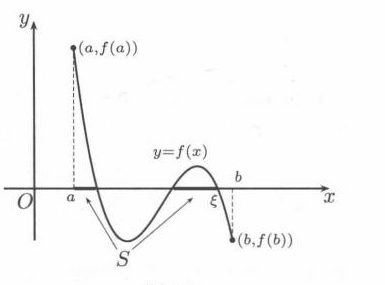
\includegraphics[width=.47\linewidth]{figures/upper/ch05/fig-5-1.png}

  图 5.1
\end{center}

现在给出介值定理和它的证明。这个定理的表达方式可有多种。如果将各种区间（包括有界区间、无限区间、开区间、闭区间以及半开半闭区间等）的共同点抽出来，则可以将介值定理表达如下：

\begin{xproposition}[5.2.2（介值定理）]
区间上的连续函数的值域必是区间（可缩为一点）。
\end{xproposition}
\begin{xproof}
设 $f\in C(I)$，其中 $I$ 为区间。为了证明 $f(I)$ 是区间，只要证明：若有 $x',x''\in I$，且 $f(x')\ne f(x'')$，则函数 $f$ 能取到在 $f(x')$ 和 $f(x'')$ 之间的每一个值。

为确定起见，只写出 $x'<x'',f(x')<c<f(x'')$ 时的证明。我们要证明，存在点 $\eta\in(x',x'')\subset I$，使得 $f(\eta)=c$。

为此作辅助函数
\[
  F(x)=f(x)-c.
\]
这时有
\[
  F(x')F(x'')=(f(x')-c)(f(x'')-c)<0.
\]
在闭区间 $[x',x'']$ 上对函数 $F(x)$ 应用连续函数的零点存在定理，就知道存在点 $\eta\in(x',x'')$，使得 $F(\eta)=0$。这就是 $f(\eta)=c$。
\end{xproof}

\begin{xremark}
介值定理的常见形式为：若 $f\in C[a,b]$，$a\le x_1<x_2\le b$，且 $f(x_1)\ne f(x_2)$，则 $f$ 可取到在 $f(x_1)$ 和 $f(x_2)$ 之间的每个值。我们将此称为介值性质。
\end{xremark}

\begin{xthought}
举例说明：区间上的函数即使处处不连续，也可以具有介值性质。
\end{xthought}
\begin{xsolution}
可以构造一个在每个非退化区间上都取遍 $\RR$ 的函数。把 $\RR$ 按等价关系
\[
 x\sim y\quad\Longleftrightarrow\quad x-y\in\QQ
\]
分成陪集。每个陪集 $x+\QQ$ 都在 $\RR$ 中稠密，而且陪集全体的势与 $\RR$ 相同。取一个双射
\[
 \Phi\colon \RR/\QQ\to\RR,
\]
并定义 $f(x)=\Phi(x+\QQ)$。

任意非退化区间都与每个陪集相交，所以它在 $f$ 下的像就是整个 $\RR$。因此 $f$ 具有介值性质。另一方面，任意点的任意邻域内 $f$ 都取遍 $\RR$，故 $f$ 在每一点都不连续。
\end{xsolution}


\begin{xremark}
介值定理只肯定在所说的条件下值域是区间，未说明什么区间。在下一节会知道在闭区间上的连续函数的值域一定是闭区间。但若定义域是其他类型的区间，包括无限区间，则连续函数的值域可以是所有可能的各种区间。
\end{xremark}

\subsection{例题}

\begin{xexample}[5.2.4]
设 $f\in C[a,b]$，且有 $f([a,b])\subset[a,b]$。证明：存在 $\xi\in[a,b]$，使得 $f(\xi)=\xi$（即 $f$ 在区间 $[a,b]$ 中有不动点）。
\end{xexample}
\begin{xproof}
引入辅助函数 $F(x)=f(x)-x$。从条件 $f([a,b])\subset[a,b]$ 可以得到
\[
  F(a)=f(a)-a\ge0,\qquad F(b)=f(b)-b\le0,
\]
因此 $F(a)F(b)\le0$。如果此式等于零，则 $f$ 以 $a$ 或 $b$ 为不动点。否则，对函数 $F$ 应用连续函数的零点存在定理，知道 $f$ 在 $(a,b)$ 中有不动点。
\end{xproof}

\begin{xremark}
这个例题是著名的 Brouwer（布劳威尔）不动点定理的特例。Brouwer 不动点定理是说，从 $n$ 维空间的球
\[
  D^n=\{x\in\RR^n\mid x_1^2+x_2^2+\cdots+x_n^2\le1\}
\]
到自身的连续映射必有不动点。在数轴上的闭区间就是一维的球。关于 Brouwer 不动点定理的一个简洁而漂亮的证明见 [40]。
\end{xremark}

\begin{xexample}[5.2.5]
若 $f\in C[a,b]$，且对每一个 $x\in[a,b]$ 存在 $y\in[a,b]$，使得 $|f(y)|\le\frac12|f(x)|$。证明：$f$ 在 $[a,b]$ 中有零点。
\end{xexample}
\begin{xproof}
任取一点 $x_0\in[a,b]$，则存在 $x_1\in[a,b]$，使 $|f(x_1)|\le\frac12|f(x_0)|$。这样继续下去，就可以归纳地得到一个数列 $\{x_n\}$，使得成立
\[
  |f(x_n)|\le\frac12|f(x_{n-1})|\le\cdots\le\frac1{2^n}|f(x_0)|.
\]
因此有 $\lim_{n\to\infty}f(x_n)=0$，即数列 $\{f(x_n)\}$ 为无穷小量。

对数列 $\{x_n\}$ 用凝聚定理，存在收敛子列 $\{x_{n_k}\}$。设极限为
\[
  \lim_{k\to\infty}x_{n_k}=\eta,
\]
则有 $\eta\in[a,b]$。由于 $f$ 在 $\eta$ 连续，就有
\[
  \lim_{k\to\infty}f(x_{n_k})=f(\eta).
\]
由于 $\{f(x_{n_k})\}$ 是 $\{f(x_n)\}$ 的子列，因此 $f(\eta)=0$。
\end{xproof}

\begin{xremark}
在构造数列 $\{x_n\}$ 时，有可能某个 $x_n$ 恰好是 $f$ 的零点。这时当然可以不必做下去。但上面写出的证明即使对这种特殊情况仍然是正确的。
\end{xremark}

\subsection{练习题}

\begin{xexercise}[1]
设 $f\in C[a,b]$，$a\le x_1<x_2<\cdots<x_n\le b$，证明：存在 $\xi\in[x_1,x_n]$，使成立
  \[
    f(\xi)=\frac{f(x_1)+f(x_2)+\cdots+f(x_n)}{n}.
  \]
\end{xexercise}
\begin{xsolution}
设
\[
 m=\min_{1\le i\le n}f(x_i),\qquad
 M=\max_{1\le i\le n}f(x_i).
\]
算术平均数
\[
 A=\frac1n\sum_{i=1}^n f(x_i)
\]
满足 $m\le A\le M$。取达到 $m,M$ 的两个点，它们都属于 $[x_1,x_n]$。由连续函数的介值定理，$f$ 在连接这两点的区间上取遍 $[m,M]$，故存在 $\xi\in[x_1,x_n]$ 使 $f(\xi)=A$。
\end{xsolution}


\begin{xexercise}[2]
设 $f$ 是定义在一个圆周上的连续函数。证明：存在一条直径，使得 $f$ 在其两端取相同的值。（试给出在圆周上的函数的连续性定义。）
\end{xexercise}
\begin{xsolution}
用参数 $\theta$ 表示圆周上的点，令 $F(\theta)$ 表示函数在该点的值。所谓圆周上的连续，是指 $F$ 为 $2\pi$ 周期连续函数。定义
\[
 h(\theta)=F(\theta)-F(\theta+\pi).
\]
则 $h$ 连续，且
\[
 h(\theta+\pi)=-h(\theta).
\]
若 $h(\theta_0)=0$，则以 $\theta_0$ 与 $\theta_0+\pi$ 为端点的直径即满足要求。否则 $h(\theta_0)$ 与 $h(\theta_0+\pi)$ 异号，由零点存在定理，在二者之间必有 $\xi$ 使 $h(\xi)=0$。故必存在所求直径。
\end{xsolution}


\begin{xexercise}[3]
若余弦多项式 $C_n(x)=\sum_{k=0}^n a_k\cos kx$ 的系数满足条件 $\sum_{k=1}^{n-1}|a_k|<a_n$，证明：$C_n(x)$ 在区间 $[0,2\pi)$ 中至少有 $2n$ 个零点。
\end{xexercise}
\begin{xsolution}
题设条件
\[
 \sum_{k=1}^{n-1}|a_k|<a_n
\]
在一般情形下不足以推出结论，因为它没有约束常数项 $a_0$。例如取 $n=2$，令
\[
 a_2=1,\qquad a_1=0,\qquad a_0=2.
\]
则 $|a_1|<a_2$ 成立，但
\[
 C_2(x)=2+\cos2x\ge1>0,
\]
在 $[0,2\pi)$ 中没有零点。因此按题设条件，命题不成立。

若把条件加强为
\[
 \sum_{k=0}^{n-1}|a_k|<|a_n|,
\]
则结论成立。令 $x_j=j\pi/n$，$j=0,1,\ldots,2n$。由于
\[
 a_n\cos(nx_j)=a_n(-1)^j
\]
且其绝对值严格大于其余各项绝对值之和，所以 $C_n(x_j)$ 的符号随 $j$ 交替。于是对每个 $j=0,1,\ldots,2n-1$，连续函数 $C_n$ 在 $(x_j,x_{j+1})$ 内至少有一个零点，从而在 $[0,2\pi)$ 中至少有 $2n$ 个零点。
\end{xsolution}


\begin{xexercise}[4]
设 $a_1,a_2,a_3>0$，且 $b_1<b_2<b_3$。证明：方程
  \[
    \frac{a_1}{x-b_1}+\frac{a_2}{x-b_2}+\frac{a_3}{x-b_3}=0
  \]
  在区间 $(b_1,b_2)$ 和 $(b_2,b_3)$ 内恰好各有一个根。
\end{xexercise}
\begin{xsolution}
记
\[
 F(x)=\frac{a_1}{x-b_1}+\frac{a_2}{x-b_2}+\frac{a_3}{x-b_3}.
\]
在每个不含 $b_i$ 的区间内 $F$ 连续。若 $x<y$ 且二者同处于 $(b_1,b_2)$ 或 $(b_2,b_3)$，则对每个 $i$，函数 $1/(x-b_i)$ 随 $x$ 严格减少；因 $a_i>0$，故 $F$ 在这两个区间上都严格减少。

在 $(b_1,b_2)$ 上，
\[
 \lim_{x\to b_1^+}F(x)=+\infty,
 \qquad
 \lim_{x\to b_2^-}F(x)=-\infty.
\]
由介值定理至少有一根，由严格单调性至多有一根，故恰有一根。同理，在 $(b_2,b_3)$ 上
\[
 \lim_{x\to b_2^+}F(x)=+\infty,
 \qquad
 \lim_{x\to b_3^-}F(x)=-\infty,
\]
也恰有一根。
\end{xsolution}


\begin{xexercise}[5]
证明：
  \begin{enumerate}[label=(\arabic*)]
    \item 奇数次多项式方程 $f(x)=x^{2n+1}+a_1x^{2n}+\cdots+a_{2n}x+a_{2n+1}=0$ 至少有一个实根；
    \item 偶数次多项式方程 $f(x)=x^{2n}+a_1x^{2n-1}+\cdots+a_{2n-1}x+a_{2n}=0$ 可以没有实根，但当 $a_{2n}<0$ 时则至少有两个实根。
  \end{enumerate}
\end{xexercise}
\begin{xsolution}
\begin{enumerate}[label=(\arabic*)]
 \item 奇数次首一多项式满足
 \[
  \lim_{x\to+\infty}f(x)=+\infty,
  \qquad
  \lim_{x\to-\infty}f(x)=-\infty.
 \]
 因此可取 $A<0<B$ 使 $f(A)<0<f(B)$。由零点存在定理，$f$ 至少有一个实根。

 \item 偶数次多项式可以没有实根，例如 $x^2+1=0$。若常数项 $a_{2n}<0$，则 $f(0)<0$，而
 \[
  \lim_{x\to\pm\infty}f(x)=+\infty.
 \]
 因而可取 $A<0<B$ 使 $f(A)>0,f(B)>0$。分别在 $[A,0]$ 和 $[0,B]$ 上应用零点存在定理，各得到一个实根；两根一负一正，故互异。
\end{enumerate}
\end{xsolution}


\begin{xexercise}[6]
证明：$x^{17}+215/(1+\cos^2 3x)=18$ 必有实根。
\end{xexercise}
\begin{xsolution}
令
\[
 F(x)=x^{17}+\frac{215}{1+\cos^2 3x}-18.
\]
$F$ 在 $\RR$ 上连续。因
\[
 F(0)=\frac{215}{2}-18>0,
\]
而
\[
 F(-2)\le -2^{17}+215-18<0,
\]
故由零点存在定理，$F$ 在 $(-2,0)$ 内有零点，即原方程必有实根。
\end{xsolution}


\begin{xexercise}[7]
若 $f\in C[a,b]$，且 $f(x)$ 只取有理数。问：$f$ 有何特点？
\end{xexercise}
\begin{xsolution}
连续函数把区间映成区间，所以 $f([a,b])$ 是 $\RR$ 中的区间。另一方面题设说该值域只含有理数。若值域中有两个不同的数 $p<q$，则区间性质要求它包含 $p,q$ 之间的所有实数，其中必有无理数，矛盾。因此值域只能退化为一个点，故 $f$ 是常值函数。
\end{xsolution}


\begin{xexercise}[8]
设 $f\in C[a,b]$，且为一对一映射。证明：
  \begin{enumerate}[label=(\arabic*)]
    \item 若 $f(a)<f(b)$，则 $f$ 严格单调增加；
    \item 若 $f(a)>f(b)$，则 $f$ 严格单调减少。
  \end{enumerate}
\end{xexercise}
\begin{xsolution}
先证明一般事实：区间上的连续一一映射必严格单调。否则存在 $x_1<x_2<x_3$，使 $f(x_2)$ 不严格位于 $f(x_1),f(x_3)$ 之间。若例如
\[
 f(x_2)>\max\{f(x_1),f(x_3)\},
\]
取 $c$ 严格介于 $\max\{f(x_1),f(x_3)\}$ 与 $f(x_2)$ 之间，则由介值定理，在 $(x_1,x_2)$ 与 $(x_2,x_3)$ 各有一点取值 $c$，与一一性矛盾。其余情形同理。因此 $f$ 严格单调。

若 $f(a)<f(b)$，严格单调不可能为减少，只能严格增加；若 $f(a)>f(b)$，则只能严格减少。这就得到 (1)、(2)。
\end{xsolution}


\begin{xexercise}[9]
设 $f\in C(-\infty,+\infty)$，且有 $f(-\infty)=A<B=f(+\infty)$，证明：对每个 $c\in(A,B)$，存在 $\xi$，使得 $f(\xi)=c$。
\end{xexercise}
\begin{xsolution}
给定 $c\in(A,B)$。由
\[
 \lim_{x\to-\infty}f(x)=A<c,
 \qquad
 \lim_{x\to+\infty}f(x)=B>c,
\]
可取 $u<v$，使
\[
 f(u)<c<f(v).
\]
函数 $f-c$ 在 $[u,v]$ 连续且两端异号，由零点存在定理存在 $\xi\in(u,v)$ 使 $f(\xi)=c$。
\end{xsolution}


\begin{xexercise}[10]
设 $f\in C[a,b)$，数列 $\{x_n\},\{y_n\}\subset[a,b)$，已知
  \[
    \lim_{n\to\infty}x_n=b,\quad \lim_{n\to\infty}y_n=b,\quad
    \lim_{n\to\infty}f(x_n)=A,\quad \lim_{n\to\infty}f(y_n)=B,
  \]
  但 $A\ne B$。证明：对每一个 $\eta\in(A,B)$，存在数列 $\{z_n\}\subset[a,b)$，满足要求
  \[
    \lim_{n\to\infty}z_n=b,\qquad \lim_{n\to\infty}f(z_n)=\eta.
  \]
\end{xexercise}
\begin{xsolution}
不妨设 $A<\eta<B$。由 $f(x_n)\to A$、$f(y_n)\to B$，当 $n$ 充分大时有
\[
 f(x_n)<\eta<f(y_n).
\]
对连接 $x_n,y_n$ 的闭区间应用介值定理，可取位于二者之间的 $z_n$，使
\[
 f(z_n)=\eta.
\]
对有限个较小的 $n$ 任意补取 $z_n\in[a,b)$ 即可。因为 $x_n\to b,y_n\to b$，而 $z_n$ 位于 $x_n,y_n$ 之间，所以夹逼得 $z_n\to b$；同时 $f(z_n)=\eta$ 对充分大的 $n$ 恒成立，故 $f(z_n)\to\eta$。
\end{xsolution}


\section{有界性定理与最值定理}

\begin{xproposition}[5.3.1（有界性定理）]
有界闭区间上的连续函数一定有界。
\end{xproposition}

\begin{xproposition}[5.3.2（最值定理）]
有界闭区间上的连续函数一定取到最大值和最小值。
\end{xproposition}

\begin{xremark}
容易看出最值定理蕴涵有界性定理，因此如果能直接证明最值定理的话，则同时也就证明了有界性定理。
\end{xremark}

\begin{xremark}
容易举出例子说明，如果将这两个定理中的有界闭区间换成其他区间，则结论都不再成立。因此这两个定理是有界闭区间上连续函数才具有的性质。由于有界闭区间与覆盖定理的紧密联系（参见第三章 §3.5 关于覆盖定理的介绍），因此可以看出，要证明这两个定理也需要实数系的基本定理。
\end{xremark}

\begin{xremark}
由连续函数的局部有界性定理知，当 $f\in C[a,b]$ 时，$f$ 在区间 $[a,b]$ 的每一点的一个邻域上有界。联系到 3.7.2 小节中的内容，可见我们已经对有界性定理作出了六个不同的证明。但是本节还将给出对这个定理的新证明。
\end{xremark}

\begin{xremark}
由最值定理再加上介值定理就得到有界闭区间上的连续函数的值域一定是闭区间的结论，这就是连续函数的值域定理：若 $f\in C[a,b]$，$M,m$ 是 $f$ 的最大值和最小值，则有
\[
  f([a,b])=[m,M].
\]
（当 $m=M$ 时值域 $[m,M]$ 退化成一点，$f$ 为常值函数。）
\end{xremark}

\subsection{定理的证明}

最值定理的证明往往是以有界性定理为基础，但下面的第一个证明却不是如此，因此它同时也可以看成是有界性定理的新证明（见 [42]）。

\begin{xexample}[5.3.1]
用确界定理和凝聚定理同时证明有界性定理和最值定理。
\end{xexample}
\begin{xproof}
由于值域 $f([a,b])$ 非空，因此可取
\[
  M=\sup f([a,b]),\qquad m=\inf f([a,b]).
\]
这里并未假定 $M,m$ 是有限数。我们的目的是证明 $M,m\in f([a,b])$。以下只写出 $M\in f([a,b])$ 的证明，它同时说明 $f$ 在 $[a,b]$ 上有上界。

从上确界的性质，在 $[a,b]$ 中存在数列 $\{x_n\}$，使得 $\lim_{n\to\infty}f(x_n)=M$。（对 $M$ 为有限数的情况，见例题 3.1.3；对 $M=+\infty$，请读者完成。）对 $\{x_n\}$ 用凝聚定理，有收敛子列 $\{x_{n_k}\}$。记该子列的极限为 $\xi$，则点 $\xi\in[a,b]$。由于 $f$ 在 $\xi$ 处连续，就有
\[
  f(\xi)=\lim_{k\to\infty}f(x_{n_k})=M.
\]
这就表示 $M\in f([a,b])$。
\end{xproof}

\begin{xremark}
请读者回答：上述证明中，闭区间的“闭”这个关键条件用在哪里？
\end{xremark}

\begin{xremark}
实际上用覆盖定理或闭区间套定理都不难同时证明有界性定理与最值定理。这是实数系基本定理的很好的练习题。请读者试之。
\end{xremark}

下一个证明说明从有界性定理到最值定理只是一步之遥。

\begin{xexample}[5.3.2]
用两次有界性定理就可以证明最值定理，关键是设计一个适当的辅助函数（见 [14]）。
\end{xexample}
\begin{xproof}
只证明其中的最大值部分。由有界性定理知道，若 $f\in C[a,b]$，则 $f$ 有上界，因此值域的上确界 $M=\sup f([a,b])$ 是有限数。我们断言 $M\in f([a,b])$。

反证法。若 $M\notin f([a,b])$，则有 $f(x)<M,\forall x\in[a,b]$。构造辅助函数
\[
  g(x)=\frac1{M-f(x)}.
\]
由于 $f\in C[a,b]$，且 $f$ 的取值始终小于 $M$，因此从连续函数的除法运算法则知道，函数 $g$ 在 $[a,b]$ 上处处连续，即也有 $g\in C[a,b]$。而且有 $g(x)>0,x\in[a,b]$。

对 $g$ 再次应用有界性定理，知道它有上界，将它记为 $M'$，则有
\[
  g(x)=\frac1{M-f(x)}\le M',\qquad \forall x\in[a,b].
\]
这就导致
\[
  f(x)\le M-\frac1{M'},\qquad \forall x\in[a,b].
\]
因此 $M-1/M'$ 是值域 $f([a,b])$ 的上界。这与 $M$ 是值域的最小上界矛盾。
\end{xproof}

\subsection{例题}

\begin{xexample}[5.3.3]
设 $f\in C(a,b)$，$f(a^+)$ 和 $f(b^-)$ 有限。证明：$f$ 在 $(a,b)$ 上有界。
\end{xexample}
\begin{xproof}
\textbf{证 1}\quad 在闭区间 $[a,b]$ 上构造辅助函数
\[
  F(x)=\begin{cases}
    f(x),&x\in(a,b),\\
    f(a^+),&x=a,\\
    f(b^-),&x=b.
  \end{cases}
\]
则可以看出 $F\in C[a,b]$。对 $F$ 应用连续函数的有界性定理，可见 $F$ 在 $[a,b]$ 上有界。因此 $f$ 在 $(a,b)$ 上也有界。
\end{xproof}

\begin{xproof}
\textbf{证 2}\quad 根据函数极限的局部有界性定理，存在 $\delta>0$，使得函数 $f$ 在 $(a,a+\delta)$ 和 $(b-\delta,b)$ 上有界。这里假定有 $a+\delta<b-\delta$ 成立。然后在闭区间 $[a+\delta,b-\delta]$ 上可以用有界性定理。这样就得到所要的结论。
\end{xproof}

\begin{xremark}
证 2 对 $a=-\infty$ 和 $b=+\infty$ 的情况同样有效。
\end{xremark}

用同样的方法可以解决下面的例题，证明从略。

\begin{xexample}[5.3.4]
设 $f\in C(a,b)$，极限 $f(a^+)$ 和 $f(b^-)$ 有限。若存在 $\xi\in(a,b)$ 使
\[
  f(\xi)>\max\{f(a^+),f(b^-)\},
\]
证明 $f$ 在 $(a,b)$ 上有最大值。
\end{xexample}

用最值定理可以对下列例题 5.2.5 给出简单得多的证明。

\begin{xexample}[5.3.5]
若 $f\in C[a,b]$，且对每一个 $x\in[a,b]$ 存在 $y\in[a,b]$，使得 $|f(y)|\le\frac12|f(x)|$。证明 $f$ 在 $[a,b]$ 中有零点。
\end{xexample}
\begin{xproof}
这时也有 $|f|\in C[a,b]$，对 $|f|$ 用最值定理，在题设条件下可见最小值只能是 0。这时的最小值点就是 $|f|$ 的零点，当然也是 $f$ 的零点。
\end{xproof}

\subsection{练习题}

\begin{xexercise}[1]
设函数 $f$ 在区间 $[a,b]$ 中只有第一类间断点，证明：$f$ 在 $[a,b]$ 上有界。
\end{xexercise}
\begin{xsolution}
任取 $x_0\in[a,b]$。若 $x_0\in(a,b)$，题设保证 $f(x_0^-),f(x_0^+)$ 都是有限数；由单侧极限的局部有界性，存在 $x_0$ 的一个邻域，使 $f$ 在去掉 $x_0$ 后有界，再把有限的函数值 $f(x_0)$ 加入即可知 $f$ 在该邻域内有界。端点处只需使用相应的单侧极限，同样得到局部有界性。

于是 $[a,b]$ 的每一点都有一个邻域，在该邻域与 $[a,b]$ 的交上 $f$ 有界。这些邻域构成 $[a,b]$ 的开覆盖。由有限覆盖定理可取有限子覆盖。有限多个局部界的最大值给出整个 $[a,b]$ 上的统一界，故 $f$ 有界。
\end{xsolution}


\begin{xexercise}[2]
若 $f\in C[a,+\infty)$，且存在有限极限 $\lim_{x\to+\infty}f(x)$。证明：$f$ 在 $[a,+\infty)$ 上有界。
\end{xexercise}
\begin{xsolution}
设
\[
 \lim_{x\to+\infty}f(x)=A\in\RR.
\]
取 $M>a$，使 $x>M$ 时 $|f(x)-A|<1$，于是尾部 $[M,+\infty)$ 上
\[
 |f(x)|\le |A|+1.
\]
在闭区间 $[a,M]$ 上，$f$ 连续，故由有界性定理有界。合并两部分即可知 $f$ 在 $[a,+\infty)$ 上有界。
\end{xsolution}


\begin{xexercise}[3]
问：是否存在从区间 (1) $(0,1)$，(2) $[0,1]$，(3) $(0,1]$ 映射到整个实数集 $\RR$ 的连续函数？（如果存在，请举出例子；如果不存在，请作出证明。）
\end{xexercise}
\begin{xsolution}
\begin{enumerate}[label=(\arabic*)]
 \item 存在。例如
 \[
  f(x)=\tan\pi\left(x-\frac12\right),\qquad 0<x<1,
 \]
 连续且值域为 $\RR$。

 \item 不存在。若 $f\in C[0,1]$，由有界性定理 $f([0,1])$ 有界，不可能等于 $\RR$。

 \item 存在。例如
 \[
  f(x)=\frac{\sin(1/x)}x,\qquad 0<x\le1.
 \]
 它在 $(0,1]$ 连续。取使 $\sin(1/x)=1$ 与 $-1$ 的两列点趋于 $0$，可见函数在 $0$ 附近既无上界又无下界。连续像是区间，而该值域同时向上、向下无界，因此只能是整个 $\RR$。
\end{enumerate}
\end{xsolution}


\begin{xexercise}[4]
问：若函数 $f$ 在区间 $[a,b]$ 上的值域为闭区间，则 $f$ 是否在 $[a,b]$ 上连续？
\end{xexercise}
\begin{xsolution}
不一定。以 $[0,1]$ 为例，定义
\[
 f(x)=\begin{cases}
  x,&0<x<1,\\
  1,&x=0,\\
  0,&x=1.
 \end{cases}
\]
则 $f([0,1])=[0,1]$，确为闭区间，但 $f$ 在 $0,1$ 都不连续。因此“值域为闭区间”不能推出连续性。
\end{xsolution}


\begin{xexercise}[5]
若 $f\in C[a,+\infty)$，且存在有限极限 $\lim_{x\to+\infty}f(x)$。证明：$f$ 在 $[a,+\infty)$ 上至少可以取到最大值或最小值中的一个。

  （可以与例题 2.2.1 作比较。）
\end{xexercise}
\begin{xsolution}
设 $\lim_{x\to+\infty}f(x)=L$。若 $f\equiv L$，则最大值、最小值都能取到。以下设 $f$ 非常值。

若存在 $x_0$ 使 $f(x_0)>L$，取
\[
 \varepsilon=\frac{f(x_0)-L}{2}>0.
\]
可取 $M>x_0$，使 $x>M$ 时
\[
 f(x)<L+\varepsilon=\frac{L+f(x_0)}2<f(x_0).
\]
因此全局最大值只能出现在闭区间 $[a,M]$ 上，而连续函数在该闭区间上取到最大值，所以 $f$ 在 $[a,+\infty)$ 上取到最大值。

若不存在这样的 $x_0$，则 $f(x)\le L$ 对所有 $x$。因为 $f$ 非常值，存在 $x_0$ 使 $f(x_0)<L$。取
\[
 \varepsilon=\frac{L-f(x_0)}2>0.
\]
可取 $M>x_0$，使 $x>M$ 时
\[
 f(x)>L-\varepsilon=\frac{L+f(x_0)}2>f(x_0).
\]
因此全局最小值只能出现在闭区间 $[a,M]$ 上，并由最值定理在该区间取得。故至少最大值或最小值之一能够取到。
\end{xsolution}


\begin{xexercise}[6]
若 $f\in C(a,b)$，且 $f(a^+)=f(b^-)=+\infty$，证明：$f$ 在 $(a,b)$ 上有最小值。
\end{xexercise}
\begin{xsolution}
取中点 $x_0=(a+b)/2$。由
\[
 f(a^+)=f(b^-)=+\infty,
\]
可取
\[
 0<\delta<\frac{b-a}{2}
\]
使在 $(a,a+\delta)$ 与 $(b-\delta,b)$ 上都有
\[
 f(x)>f(x_0)+1.
\]
在闭区间 $[a+\delta,b-\delta]$ 上，$f$ 由最值定理取到最小值 $m$。因 $x_0$ 属于该闭区间，故 $m\le f(x_0)$；而两端邻近部分的函数值都大于 $f(x_0)+1>m$。因此 $m$ 也是整个 $(a,b)$ 上的最小值。
\end{xsolution}


\begin{xexercise}[7]
若 $f\in C(a,b)$，且 $f(a^+)=f(b^-)$，证明：$f$ 在 $(a,b)$ 上至少可以取到最大值或最小值中的一个。
\end{xexercise}
\begin{xsolution}
记共同的端点极限为 $L$。

若 $L\in\RR$，定义
\[
 F(a)=F(b)=L,\qquad F(x)=f(x)\quad(a<x<b).
\]
则 $F\in C[a,b]$，故取到最大值和最小值。若 $f\equiv L$，结论当然成立；否则存在一点函数值大于 $L$ 或小于 $L$。前一种情况下 $F$ 的最大值必在 $(a,b)$ 取得，后一种情况下最小值必在 $(a,b)$ 取得。

若 $L=+\infty$，由上一题 $f$ 取到最小值；若 $L=-\infty$，对 $-f$ 应用上一题，得到 $f$ 取到最大值。故各种情况下至少能取到最大值或最小值中的一个。
\end{xsolution}


\begin{xexercise}[8]
若 $f\in C(-\infty,+\infty)$，$\lim_{x\to\pm\infty}f(x)=+\infty$，且 $f(x)$ 的最小值 $f(a)<a$。证明：复合函数 $f(f(x))$ 至少在两个点上取到它的最小值。
\end{xexercise}
\begin{xsolution}
设 $m=f(a)$ 是 $f$ 的全局最小值，且 $m<a$。因为 $f(x)\to+\infty$ 当 $x\to\pm\infty$，连续函数的值域为
\[
 f(\RR)=[m,+\infty).
\]
特别地 $a\in[m,+\infty)=f(\RR)$。对复合函数 $F=f\circ f$，其取值为 $f$ 在 $[m,+\infty)$ 上的取值。由于 $a\in[m,+\infty)$ 且 $f(a)=m$ 是 $f$ 的全局最小值，故
\[
 \min_{x\in\RR}F(x)=m,
\]
而 $F(x)=m$ 当且仅当 $f(x)$ 是 $f$ 的某个最小值点；特别地，只要 $f(x)=a$ 就有 $F(x)=m$。

由 $f(a)=m<a$，再利用 $f(x)\to+\infty$ 当 $x\to-\infty$ 与 $x\to+\infty$，分别在 $a$ 的左、右两侧用介值定理，可得到
\[
 x_1<a<x_2,
 \qquad f(x_1)=f(x_2)=a.
\]
于是
\[
 F(x_1)=F(x_2)=f(a)=m,
\]
所以复合函数至少在两个不同点取到它的最小值。
\end{xsolution}


\begin{xexercise}[9]
求出 Dirichlet 函数和 Riemann 函数的所有极值点和最值点。

  （关于极值与极值点的定义见 7.1.1 小节。）
\end{xexercise}
\begin{xsolution}
对 Dirichlet 函数 $D$，有 $0\le D\le1$。每个有理点的函数值为 $1$，故每个有理点都是极大值点，同时也是最大值点；每个无理点函数值为 $0$，故每个无理点都是极小值点，同时也是最小值点。所有这些极值均非严格极值。

对 Riemann 函数 $R$，有 $R\ge0$。每个无理点函数值为 $0$，因此每个无理点都是极小值点和最小值点。若 $x_0=p/q$ 为既约有理数，$q>0$，则 $R(x_0)=1/q$。在 $x_0$ 的充分小邻域内，除 $x_0$ 外不存在分母不超过 $q$ 的既约有理数，所以邻域内其余点均有
\[
 R(x)<\frac1q=R(x_0).
\]
因此每个有理点都是严格极大值点。Riemann 函数的全局最大值为 $1$，恰在分母 $q=1$ 的有理点，即所有整数处取得；全局最小值为 $0$，在所有无理点取得。
\end{xsolution}


\section{一致连续性与 Cantor 定理}

函数的一致连续性是一个比较精细的概念。可以认为这个概念是由于数学分析内部理论发展的需要而产生的。因此我们在下面先对这个概念列出要点，提出几个思考题，然后给出 Cantor（康托尔）定理的证明，并讨论其应用。

\subsection{内容提要}

关于函数的一致连续性的要点如下。

\begin{enumerate}
  \item 定义：函数 $f$ 在区间 $I$ 上一致连续，如果对每一个 $\varepsilon>0$，存在 $\delta>0$，使得当 $x',x''\in I$ 且 $|x'-x''|<\delta$ 时，成立 $|f(x')-f(x'')|<\varepsilon$。
  \item 若 $f$ 在区间 $I$ 上一致连续，则 $f$ 在 $I$ 上一定连续。
  \item 若 $f$ 在区间 $I$ 上一致连续，又有区间 $J\subset I$，则 $f$ 在 $J$ 上也一致连续。
  \item 函数 $f$ 在区间 $I$ 上连续就是在 $I$ 的每一点连续，因此这是一个逐点（point-wise）定义的概念。从本质上看，连续性是个局部概念。但是 $f$ 在区间 $I$ 上的一致连续性则是由 $f$ 和 $I$ 两者共同确定的整体性概念。与此类似的是函数在区间上的有界性等概念。
  \item Cantor 定理：有界闭区间上的连续函数必在这个区间上一致连续。
  \item 有界开区间 $(a,b)$ 上的连续函数 $f$ 在 $(a,b)$ 上一致连续的充分必要条件是存在两个有限的单侧极限 $f(a^+)$ 和 $f(b^-)$（见下面的例题 5.4.5）。
  \item 有界区间（不论开或闭或半开半闭）上的一致连续函数一定有界（留作练习）。
\end{enumerate}

\subsection{思考题}

\begin{xthought}[1]
写出函数 $f$ 在区间 $I$ 上不一致连续的正面叙述。
\end{xthought}
\begin{xsolution}
正面叙述为：存在 $\varepsilon_0>0$，使得对每个 $\delta>0$，总能找到 $x',x''\in I$ 满足
\[
 |x'-x''|<\delta,
 \qquad
 |f(x')-f(x'')|\ge\varepsilon_0.
\]
等价地，存在 $\varepsilon_0>0$ 与两列点 $x_n',x_n''\in I$，使
\[
 |x_n'-x_n''|\to0,
 \qquad
 |f(x_n')-f(x_n'')|\ge\varepsilon_0.
\]
\end{xsolution}


\begin{xthought}[2]
判断对或错：$f$ 在区间 $[a,b)$ 上连续，则 $f$ 在 $[a,b)$ 上一致连续。
\end{xthought}
\begin{xsolution}
错误。例如在 $[0,1)$ 上取
\[
 f(x)=\frac1{1-x}.
\]
它在 $[0,1)$ 上连续，但当 $x\to1^-$ 时无界。若它一致连续，则有界半开区间上的一致连续函数应有界，矛盾。也可直接取 $x_n=1-1/n$、$y_n=1-1/(2n)$ 构造反例。
\end{xsolution}


\begin{xthought}[3]
判断对或错：$f$ 在区间 $(a,b)$ 内的每一个闭子区间上连续，则 $f$ 在 $(a,b)$ 上一致连续。
\end{xthought}
\begin{xsolution}
错误。函数 $f(x)=1/x$ 在 $(0,1)$ 内每个闭子区间上都连续，但在 $(0,1)$ 上不一致连续。
\end{xsolution}


\begin{xthought}[4]
判断对或错：$f$ 在区间 $(a,b)$ 上连续，又有 $a<c<d<b$，则 $f$ 在区间 $(c,d)$ 上一致连续。
\end{xthought}
\begin{xsolution}
正确。因为 $a<c<d<b$，$f$ 在闭区间 $[c,d]\subset(a,b)$ 上连续。由 Cantor 定理，$f$ 在 $[c,d]$ 上一致连续，所以其限制在 $(c,d)$ 上也一致连续。
\end{xsolution}


\subsection{Cantor 定理的证明}

\begin{xexample}[5.4.1]
用覆盖定理证明 Cantor 定理。
\end{xexample}
\begin{xproof}
$\forall\varepsilon>0$ 和 $x_0\in[a,b]$，由于 $f$ 在 $x_0$ 连续，存在 $\delta_0>0$，当 $x\in O_{\delta_0}(x_0)\cap[a,b]$ 时，成立 $|f(x)-f(x_0)|<\frac12\varepsilon$。因此当 $x',x''\in O_{\delta_0}(x_0)\cap[a,b]$ 时，就有
\[
  |f(x')-f(x'')|\le|f(x')-f(x_0)|+|f(x_0)-f(x'')|<\frac12\varepsilon+\frac12\varepsilon=\varepsilon.
\]
对每个点 $x\in[a,b]$ 都这样做，就得到区间 $[a,b]$ 的一个开覆盖。这里出现了一个困难，即如果对这个开覆盖直接应用覆盖定理的话，则难以完成定理的证明（读者可以试一下，看看困难何在）。再次应用例题 3.5.3（即加强形式的覆盖定理），将其中的 Lebesgue 数记为 $\eta$。当 $x',x''\in[a,b]$，且 $|x'-x''|<\eta$ 时，在开覆盖中存在一个开区间，它覆盖点 $x'$ 和 $x''$。由上述构造方法，就知道成立
\[
  |f(x')-f(x'')|<\varepsilon.
\]
这样就已经证明了 $f$ 在 $[a,b]$ 上一致连续。
\end{xproof}

\begin{xexample}[5.4.2]
用凝聚定理证明 Cantor 定理。
\end{xexample}
\begin{xproof}
用反证法。设 $f\in C[a,b]$，但在 $[a,b]$ 上不一致连续。应用 §1.4 的对偶法则，可以得到不一致连续的正面叙述：$\exists\varepsilon_0>0,\ \forall\delta>0,\ \exists x',x''\in[a,b],|x'-x''|<\delta$，使得 $|f(x')-f(x'')|\ge\varepsilon_0$ 成立。

取 $\delta_n=1/n$，将对应的点 $x',x''$ 记为 $x_n$ 和 $x_n'$。并对每一个 $n\in\NN_+$ 都这样做，就得到区间 $[a,b]$ 中的两个数列 $\{x_n\}$ 和 $\{x_n'\}$，使得
\[
  |x_n-x_n'|<\frac1n,\qquad |f(x_n)-f(x_n')|\ge\varepsilon_0,\quad \forall n\in\NN_+.
\]
对数列 $\{x_n\}$ 用凝聚定理，知道存在收敛子列 $\{x_{n_k}\}$。记它的极限为 $\xi$，即有
\[
  \lim_{k\to\infty}x_{n_k}=\xi.
\]
由于
\[
  x_{n_k}-\frac1{n_k}<x_{n_k}'<x_{n_k}+\frac1{n_k},
\]
以及 $n_k\ge k$，因此数列 $\{x_n'\}$ 的对应子列 $\{x_{n_k}'\}$ 也收敛于 $\xi$，即有
\[
  \lim_{k\to\infty}x_{n_k}'=\xi.
\]
由于 $f$ 在点 $\xi$ 连续，因此对 $\varepsilon_0$，存在 $\eta>0$，当 $x',x''\in O_\eta(\xi)$ 时，成立 $|f(x')-f(x'')|<\varepsilon_0$。但当 $k$ 充分大时，就有 $x_{n_k},x_{n_k}'\in O_\eta(\xi)$。这样就和
\[
  |f(x_{n_k})-f(x_{n_k}')|\ge\varepsilon_0
\]
矛盾。
\end{xproof}

\subsection{例题}

\begin{xexample}[5.4.3]
根据定义证明：
\begin{enumerate}[label=(\arabic*)]
  \item 对于满足 $0<\eta<1$ 的每个 $\eta$，$f(x)=1/x$ 在 $[\eta,1)$ 上一致连续；
  \item $f(x)=1/x$ 在开区间 $(0,1)$ 上不一致连续。
\end{enumerate}
\end{xexample}
\begin{xproof}
(1) 对 $x',x''\in[\eta,1)$，有
\[
  |f(x')-f(x'')|=\left|\frac1{x'}-\frac1{x''}\right|=\frac{|x'-x''|}{x'x''}\le\frac{|x'-x''|}{\eta^2}.
\]
因此对 $\varepsilon>0$，只要取
\[
  \delta=\eta^2\varepsilon,
\]
就可以使得 $x',x''\in[\eta,1)$ 且 $|x'-x''|<\delta$ 时，成立 $|1/x'-1/x''|<\varepsilon$。这表明 $f(x)=1/x$ 在区间 $[\eta,1)$ 上一致连续。

(2) 用反证法。设 $f(x)=1/x$ 在区间 $(0,1)$ 上一致连续。则对 $\varepsilon=1$，存在 $\delta>0$，使得当 $x',x''\in(0,1)$ 且 $|x'-x''|<\delta$ 时，成立
\[
  |f(x')-f(x'')|=\left|\frac1{x'}-\frac1{x''}\right|=\frac{|x'-x''|}{x'x''}<1.
\]
设 $n\ge2$，并令
\[
  x'=\frac1n,\qquad x''=\frac1{2n},
\]
则有
\[
  |x'-x''|=\frac1{2n},\qquad |f(x')-f(x'')|=n\ge2>1.
\]
因此只要取 $n>1/(2\delta)$，就引出矛盾，所以 $f(x)=1/x$ 在 $(0,1)$ 上不一致连续。
\end{xproof}

\begin{xremark}
若初学者对理解一致连续性概念有困难，建议先将本例题彻底搞清楚。利用 $y=1/x$ 的几何图形，可以体会出一致连续性与函数的“陡度”有关。从证明也可看出，本例中的困难完全发生在点 $x=0$ 的右侧邻近。
\end{xremark}

\begin{xremark}
可以类比：同一个函数 $f(x)=1/x$ 在 $(0,1)$ 上无界，但在 $(0,1)$ 内的每一个闭子区间上有界。由此可见，有界性和一致连续性是属于同一类型的概念，即整体性质，也就是说与函数在整个区间上的性质有关。而连续性、极限的存在性等是局部性质，即只与所考虑的点附近的函数性质有关。
\end{xremark}

\begin{xexample}[5.4.4]
若函数 $f$ 在区间 $(a,b]$ 和 $[b,c)$ 上分别为一致连续，证明：$f$ 在 $(a,c)$ 上一致连续。
\end{xexample}
\begin{xproof}
对 $\varepsilon>0$，由条件知道存在 $\delta_1>0$，使得当 $x',x''\in(a,b]$ 且 $|x'-x''|<\delta_1$ 时，成立 $|f(x')-f(x'')|<\varepsilon/2$。又存在 $\delta_2>0$，使得当 $x',x''\in[b,c)$ 且 $|x'-x''|<\delta_2$ 时，成立 $|f(x')-f(x'')|<\varepsilon/2$。

取 $\delta=\min\{\delta_1,\delta_2\}$。我们断言：当 $x',x''\in(a,c)$ 且 $|x'-x''|<\delta$ 时，成立 $|f(x')-f(x'')|<\varepsilon$。

先考虑 $x'<b<x''$ 的情况。这时从 $|x'-x''|<\delta$ 推出 $|x'-b|<\delta_1,|x''-b|<\delta_2$ 成立，因此
\[
  |f(x')-f(x'')|\le|f(x')-f(b)|+|f(b)-f(x'')|<\frac\varepsilon2+\frac\varepsilon2=\varepsilon.
\]
对于其他情况，即 $x',x''$ 同属区间 $(a,b]$ 或 $[b,c)$，结论是明显的。因此就证明了 $f$ 在 $(a,c)$ 上是一致连续的。
\end{xproof}

\begin{xremark}
用下一个例题的结果可立即导致本题的结论，但上面的证明只涉及一致连续性的定义，完全是初等的。而下一个例题的证明则需要用到 Cantor 定理和 Cauchy 收敛准则，要“高级”得多。
\end{xremark}

\begin{xexample}[5.4.5]
证明：有界开区间 $(a,b)$ 上的连续函数 $f$ 在 $(a,b)$ 上一致连续的充分必要条件是存在两个有限的单侧极限 $f(a^+)$ 和 $f(b^-)$。
\end{xexample}
\begin{xproof}
先证充分性。在闭区间 $[a,b]$ 上构造辅助函数
\[
  F(x)=\begin{cases}
    f(a^+),&x=a,\\
    f(x),&x\in(a,b),\\
    f(b^-),&x=b.
  \end{cases}
\]
则可以看出 $F\in C[a,b]$。对 $F$ 应用 Cantor 定理，可见 $F$ 在 $[a,b]$ 上一致连续，因此 $f$ 在 $(a,b)$ 上也一致连续。（这与例题 5.3.3 的第一个证明完全相同。）

再证必要性。不妨只写出存在 $f(a^+)$ 的证明。对 $\varepsilon>0$，由于 $f$ 在 $(a,b)$ 上一致连续，因此存在 $\delta>0$，使得当 $x',x''\in(a,b)$，且 $|x'-x''|<\delta$ 时，成立 $|f(x')-f(x'')|<\varepsilon$。

因此当 $x',x''\in(a,a+\delta)$ 时，就有 $|f(x')-f(x'')|<\varepsilon$ 成立。应用关于右侧极限的 Cauchy 收敛准则（命题 4.2.5），可见存在极限 $f(a^+)$。
\end{xproof}

以下讨论在无限区间上函数的一致连续性。首先有如下的一个基本结果。

\begin{xexample}[5.4.6]
设 $f\in C[a,+\infty)$，且存在有限极限 $f(+\infty)=A$。证明：$f$ 在 $[a,+\infty)$ 上一致连续。
\end{xexample}
\begin{xproof}
对 $\varepsilon>0$，存在 $M>a$，当 $x>M$ 时成立 $|f(x)-A|<\frac12\varepsilon$。又利用 Cantor 定理，知道 $f$ 在 $[a,M+1]$ 上一致连续。因此对上述 $\varepsilon$，存在 $\delta>0$，使得当 $x',x''\in[a,M+1]$ 且 $|x'-x''|<\delta$ 时，成立 $|f(x')-f(x'')|<\varepsilon$。

不妨假定上述 $\delta<1$。我们断言：当 $x',x''\in[a,+\infty)$ 且 $|x'-x''|<\delta$ 时，成立 $|f(x')-f(x'')|<\varepsilon$。

实际上，如 $x',x''\in[a,M+1]$，则已无问题。又若 $x',x''>M$，则有
\[
  |f(x')-f(x'')|\le|f(x')-A|+|A-f(x'')|<\frac\varepsilon2+\frac\varepsilon2=\varepsilon.
\]
由于 $|x'-x''|<\delta<1$，只可能发生以上两种情况。
\end{xproof}

\begin{xremark}
在教学中发现，学生经常会对上述命题作出以下错误的证明：

“$\forall\varepsilon>0$，由于 $f(+\infty)=A$，因此存在 $M>a$，使当 $x',x''\in[M,+\infty)$ 时，$|f(x')-f(x'')|<\varepsilon$。由 $\varepsilon$ 的任意性，得 $f$ 在 $[M,+\infty)$ 上一致连续，再由 Cantor 定理，$f$ 在 $[a,M+1]$ 上一致连续，所以 $f$ 在 $[a,+\infty)$ 上一致连续。”

请读者思考上述证明错在哪里。
\end{xremark}

但是对于在无限区间上的函数的一致连续性来说，上述极限 $f(+\infty)$ 的存在并非必要。函数的有界性也不是必要的。例如 $f(x)=ax+b$ 在 $(-\infty,+\infty)$ 上一致连续。再举一个更有意义的例题。

\begin{xexample}[5.4.7]
证明：函数 $\sqrt{x}$ 在区间 $(0,+\infty)$ 上一致连续。
\end{xexample}
\begin{xproof}
\textbf{证 1}\quad 先分别证明 $\sqrt{x}$ 在区间 $(0,1]$ 和 $[1,+\infty)$ 上的一致连续性。

从例题 5.4.5 或在 $[0,1]$ 上用 Cantor 定理，就知道 $\sqrt{x}$ 在 $(0,1]$ 上一致连续。在区间 $[1,+\infty)$ 上，可以从
\[
  |\sqrt{x'}-\sqrt{x''}|=\frac{|x'-x''|}{\sqrt{x'}+\sqrt{x''}}\le\frac12|x'-x''|
\]
推出 $\sqrt{x}$ 在 $[1,+\infty)$ 上一致连续。

然后可以用例题 5.4.4 中的方法合并两个区间，得到所要的结论（从略）。
\end{xproof}

\begin{xproof}
\textbf{证 2}\quad 利用一个可以直接验证的不等式，即当 $0\le b<a$ 时成立
\[
  \sqrt a-\sqrt b\le\sqrt{a-b},
\]
就有对任何 $x',x''\ge0$ 成立的不等式
\[
  |\sqrt{x'}-\sqrt{x''}|\le\sqrt{|x'-x''|}.
\]
因此对 $\varepsilon>0$，只要取 $\delta=\varepsilon^2$，就可以直接得到所要的结论。
\end{xproof}

在无限区间上的有界函数也可以不一致连续。下面就是一个典型例子。

\begin{center}
  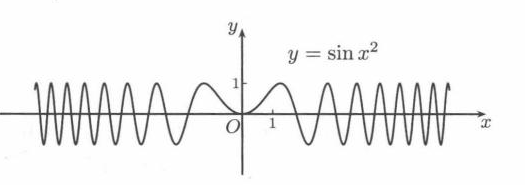
\includegraphics[width=.62\linewidth]{figures/upper/ch05/fig-5-2.png}

  图 5.2
\end{center}

\begin{xexample}[5.4.8]
证明：函数 $\sin x^2$ 在 $(-\infty,+\infty)$ 上不一致连续。
\end{xexample}
\begin{xproof}
用反证法。设 $\sin x^2$（如图 5.2 所示）在 $(-\infty,+\infty)$ 上一致连续，则 $\forall\varepsilon>0$，存在 $\delta>0$，当 $x_1,x_2$ 满足 $|x_1-x_2|<\delta$ 时，成立
\begin{equation}
  |\sin x_1^2-\sin x_2^2|<\varepsilon.
  \tag{5.3}
  \label{eq:5.3}
\end{equation}
设 $n\in\NN_+$，令
\[
  x_1=\sqrt{n\pi},\qquad x_2=\sqrt{n\pi+\frac\pi2},
\]
则 $\sin x_1^2=0,\sin x_2^2=\pm1$。因此当 $\varepsilon<1$ 时，不等式 (5.3) 不能成立。

但又有
\[
  |x_1-x_2|=\frac{\pi/2}{\sqrt{n\pi}+\sqrt{n\pi+\pi/2}},
\]
因此可以看出，当 $n$ 充分大时就有 $|x_1-x_2|<\delta$ 成立。由此引出矛盾。
\end{xproof}

\subsection{练习题}

\begin{xexercise}[1]
若 $f$ 在区间 $I$ 上定义，且存在 $L>0$，使得对任意 $x_1,x_2\in I$ 成立 $|f(x_1)-f(x_2)|\le L|x_1-x_2|$，则称 $f$ 在 $I$ 上满足 Lipschitz（利普希茨）条件。证明：在区间 $I$ 上满足 Lipschitz 条件的函数必是一致连续函数。
\end{xexercise}
\begin{xsolution}
给定 $\varepsilon>0$。若 $L>0$，取
\[
 \delta=\frac\varepsilon L.
\]
当 $x_1,x_2\in I$ 且 $|x_1-x_2|<\delta$ 时，由 Lipschitz 条件
\[
 |f(x_1)-f(x_2)|\le L|x_1-x_2|<\varepsilon.
\]
所以 $f$ 在 $I$ 上一致连续。
\end{xsolution}


\begin{xexercise}[2]
根据一致连续性的定义直接证明：若 $f$ 在 $(a,b)$ 上一致连续，则 $f$ 有界。
\end{xexercise}
\begin{xsolution}
这里 $a,b$ 为有限端点。取 $\varepsilon=1$。由一致连续性存在 $\delta>0$，使 $x,y\in(a,b)$ 且 $|x-y|<\delta$ 时
\[
 |f(x)-f(y)|<1.
\]
把有限区间 $(a,b)$ 分成有限个长度小于 $\delta$ 的小区间，并在每个非空小区间中选一点 $\xi_j$。若 $x$ 落在第 $j$ 个小区间，则
\[
 |f(x)|\le |f(\xi_j)|+1.
\]
有限个数 $|f(\xi_j)|+1$ 的最大值就是 $f$ 的一个全局界。因此 $f$ 有界。

若把端点允许为无穷，则结论一般不成立，例如 $f(x)=x$ 在 $\RR$ 上一致连续但无界。
\end{xsolution}


\begin{xexercise}[3]
\begin{enumerate}[label=(\arabic*)]
    \item 设 $f,g$ 在区间 $I$ 上均为一致连续，问：它们的线性组合 $af+bg$ 和乘积 $fg$ 在 $I$ 上是否一致连续？
    \item 设 $f$ 在区间 $I_1$ 上一致连续，$g$ 在区间 $I_2$ 上一致连续，且区间 $I_2$ 包含了 $f$ 的值域，问：复合函数 $g\circ f$ 在区间 $I_1$ 上是否一致连续？
  \end{enumerate}
\end{xexercise}
\begin{xsolution}
\begin{enumerate}[label=(\arabic*)]
 \item 线性组合一定一致连续。事实上，给定 $\varepsilon>0$，分别利用 $f,g$ 的一致连续性使
 \[
  |a|\,|f(x)-f(y)|<\frac\varepsilon2,
  \qquad
  |b|\,|g(x)-g(y)|<\frac\varepsilon2
 \]
 （系数为零时相应项忽略），再取两个 $\delta$ 的较小者即可。

 乘积在一般区间上不一定一致连续。例如在 $I=\RR$ 上 $f(x)=g(x)=x$ 都一致连续，但 $fg=x^2$ 不一致连续。若另外知道 $I$ 有界，则 $f,g$ 因一致连续而有界，此时由
 \[
  |f(x)g(x)-f(y)g(y)|
  \le |f(x)|\,|g(x)-g(y)|+|g(y)|\,|f(x)-f(y)|
 \]
 可知乘积也一致连续。

 \item 一定一致连续。给定 $\varepsilon>0$，由 $g$ 在 $I_2$ 上一致连续，存在 $\eta>0$，使 $u,v\in I_2$ 且 $|u-v|<\eta$ 时
 \[
  |g(u)-g(v)|<\varepsilon.
 \]
 再由 $f$ 在 $I_1$ 上一致连续，存在 $\delta>0$，使 $x,y\in I_1$ 且 $|x-y|<\delta$ 时
 \[
  |f(x)-f(y)|<\eta.
 \]
 因 $f(I_1)\subset I_2$，故此时
 \[
  |g(f(x))-g(f(y))|<\varepsilon.
 \]
\end{enumerate}
\end{xsolution}


\begin{xexercise}[4]
设 $f\in C(-\infty,+\infty)$，且为周期函数。证明：$f$ 在 $(-\infty,+\infty)$ 上一致连续。
\end{xexercise}
\begin{xsolution}
设 $T>0$ 是 $f$ 的一个周期。由 Cantor 定理，$f$ 在闭区间 $[0,3T]$ 上一致连续。给定 $\varepsilon>0$，取相应的 $\delta>0$，并可令 $\delta<T$。

任取 $x,y\in\RR$ 且 $|x-y|<\delta$。可取整数 $k$，使
\[
 x-kT\in[T,2T).
\]
于是因为 $|x-y|<T$，有
\[
 y-kT\in(0,3T).
\]
利用周期性与 $[0,3T]$ 上的一致连续性，
\[
 |f(x)-f(y)|
 =|f(x-kT)-f(y-kT)|<\varepsilon.
\]
所以 $f$ 在整个 $\RR$ 上一致连续。
\end{xsolution}


\begin{xexercise}[5]
\begin{enumerate}[label=(\arabic*)]
    \item 设 $f\in C[0,+\infty)$，且有 $\lim_{x\to+\infty}[f(x)-(ax+b)]=0$，证明 $f$ 在 $[0,+\infty)$ 上一致连续；
    \item 若将 (1) 中的 $ax+b$ 换成 $ax^2+bx+c$，结论是否成立？
    \item 又若将 $ax+b$ 换成某个函数 $g(x)$，问：当 $g(x)$ 具有什么性质时 (1) 中的结论仍成立？
  \end{enumerate}
\end{xexercise}
\begin{xsolution}
\begin{enumerate}[label=(\arabic*)]
 \item 写成
 \[
  f(x)=ax+b+r(x),
  \qquad r(x)=f(x)-(ax+b).
 \]
 则 $r\in C[0,+\infty)$ 且 $r(x)\to0$。由例题 5.4.6，$r$ 在 $[0,+\infty)$ 上一致连续；线性函数 $ax+b$ 满足 Lipschitz 条件，也一致连续。因此二者之和 $f$ 一致连续。

 \item 一般不成立。取 $f(x)=x^2$，则
 \[
  f(x)-(x^2)=0,
 \]
 完全满足相应的渐近条件，但 $x^2$ 在 $[0,+\infty)$ 上不一致连续。

 \item 若 $g$ 在 $[0,+\infty)$ 上一致连续，则 (1) 的结论仍成立。事实上，令
 \[
  r(x)=f(x)-g(x).
 \]
 因 $g$ 一致连续，所以 $g$ 连续，从而 $r\in C[0,+\infty)$；又由题设 $r(x)\to0$。例题 5.4.6 表明 $r$ 一致连续；再由 $g$ 一致连续，得到 $f=g+r$ 一致连续。

 在假定 $g$ 连续的条件下，这一条件也是必要的：若 $f$ 一致连续，则 $r=f-g$ 由上述理由一致连续，从而 $g=f-r$ 也一致连续。因此，此时结论成立的充分必要条件就是 $g$ 一致连续。
\end{enumerate}
\end{xsolution}


\begin{xexercise}[6]
证明：当 $n>1$ 时，$x^n$ 在 $[0,+\infty)$ 上不一致连续。
\end{xexercise}
\begin{xsolution}
这里 $n>1$ 不必是整数。取
\[
 x_m=m,
 \qquad
 y_m=(m^n+1)^{1/n}.
\]
则
\[
 y_m^n-x_m^n=1.
\]
又因 $0<1/n<1$，对 $t\ge0$ 有 $(1+t)^{1/n}\le1+t$，故
\[
 0<y_m-x_m
 =m\left[\left(1+\frac1{m^n}\right)^{1/n}-1\right]
 \le \frac1{m^{n-1}}\to0.
\]
因此两点距离趋于 $0$，而函数值之差恒为 $1$，与一致连续性的序列判据矛盾。所以 $x^n$ 在 $[0,+\infty)$ 上不一致连续。
\end{xsolution}


\begin{xexercise}[7]
证明：$f(x)=\ln x$ 在 $(1,+\infty)$ 一致连续，但在 $(0,1)$ 上不一致连续。
\end{xexercise}
\begin{xsolution}
在 $(1,+\infty)$ 上，设 $1<x<y$。由基本不等式 $\ln(1+t)\le t\ (t>-1)$，
\[
 0<\ln y-\ln x
 =\ln\left(1+\frac{y-x}{x}\right)
 \le\frac{y-x}{x}<y-x.
\]
故 $\ln x$ 在 $(1,+\infty)$ 上满足 Lipschitz 常数 $1$ 的估计，因而一致连续。

在 $(0,1)$ 上取
\[
 x_n=\frac1n,
 \qquad y_n=\frac1{2n}.
\]
则 $|x_n-y_n|\to0$，但
\[
 |\ln x_n-\ln y_n|=\ln2.
\]
故不一致连续。
\end{xsolution}


\begin{xexercise}[8]
\begin{enumerate}[label=(\arabic*)]
    \item 证明：函数 $f(x)=|\sin x|/x$ 在区间 $(-1,0)$ 和 $(0,1)$ 均为一致连续，但在 $(-1,0)\cup(0,1)$ 上不一致连续（注意 $(-1,0)\cup(0,1)$ 不是一个区间）；
    \item 若函数 $f$ 在区间 $(a,b)$ 和 $[b,c)$ 上分别为一致连续，问：$f$ 在 $(a,c)$ 上是否一致连续？
  \end{enumerate}
\end{xexercise}
\begin{xsolution}
\begin{enumerate}[label=(\arabic*)]
 \item 在 $(0,1)$ 上
 \[
  f(x)=\frac{|\sin x|}{x}=\frac{\sin x}{x}\longrightarrow1
  \qquad(x\to0^+),
 \]
 因而可连续延拓到 $[0,1]$；在 $(-1,0)$ 上
 \[
  f(x)=\frac{|\sin x|}{x}=-\frac{\sin x}{x}\longrightarrow-1
  \qquad(x\to0^-),
 \]
 也可连续延拓到 $[-1,0]$。由 Cantor 定理，两侧分别一致连续。

 但取 $x_n=-1/n,y_n=1/n$，则 $|x_n-y_n|\to0$，而
 \[
  f(x_n)\to-1,
  \qquad f(y_n)\to1,
 \]
 故在并集 $(-1,0)\cup(0,1)$ 上不一致连续。

 \item 不一定。令
 \[
  f(x)=\begin{cases}0,&a<x<b,\\1,&b\le x<c.
  \end{cases}
 \]
 则 $f$ 在 $(a,b)$ 与 $[b,c)$ 上分别为常值函数，故分别一致连续，但在 $b$ 处不连续，所以在 $(a,c)$ 上不可能一致连续。这里关键在于第一段不包含公共点 $b$；这与例题 5.4.4 的 $(a,b]$、$[b,c)$ 情形不同。
\end{enumerate}
\end{xsolution}


\begin{xexercise}[9]
讨论以下函数在指定区间上是否一致连续（可参考图 4.2）：
  \begin{enumerate}[label=(\arabic*)]
    \item 在区间 $(0,1)$ 上的函数 $x\sin(1/x)$；
    \item 在区间 $(0,+\infty)$ 上的函数 $\sin x/x$；
    \item 在区间 $[0,+\infty)$ 上的函数 $x\sin x$。
  \end{enumerate}
\end{xexercise}
\begin{xsolution}
\begin{enumerate}[label=(\arabic*)]
 \item $x\sin(1/x)$ 在 $x\to0^+$ 时趋于 $0$，故令 $f(0)=0$ 后可连续延拓到 $[0,1]$。由 Cantor 定理，它在 $(0,1)$ 上一致连续。

 \item 令 $f(0)=1$，则 $\sin x/x$ 连续延拓到 $[0,+\infty)$，而且 $f(x)\to0$ 当 $x\to+\infty$。由例题 5.4.6，它在 $[0,+\infty)$ 上一致连续，故在 $(0,+\infty)$ 上也一致连续。

 \item 不一致连续。取
 \[
  x_n=n\pi,
  \qquad y_n=n\pi+\frac1n.
 \]
 则 $|x_n-y_n|=1/n\to0$，而
 \[
  x_n\sin x_n=0,
 \]
 且
 \[
  |y_n\sin y_n|
  =\left(n\pi+\frac1n\right)\sin\frac1n
  \longrightarrow\pi.
 \]
 因此函数值之差不趋于 $0$，故 $x\sin x$ 在 $[0,+\infty)$ 上不一致连续。
\end{enumerate}
\end{xsolution}


\section{单调函数}

\subsection{基本性质}

单调函数是数学分析中除连续函数类之外的又一类重要函数。本小节列出关于单调函数的主要结果。

首先，从单调函数的单侧极限存在定理（命题 4.2.2）可以知道：

\begin{xproposition}[5.5.1]
单调函数的间断点是跳跃点，即在该处有两个不等的单侧极限。
\end{xproposition}
\begin{xproof}
不妨只讨论 $f$ 是 $(a,b)$ 上的单调增加函数的情况。设 $x_0\in(a,b)$ 是 $f$ 的间断点，任取 $x_0$ 两侧的点 $x,x'$（$x<x_0<x'$），则成立
\begin{equation}
  f(x)\le f(x_0)\le f(x').
  \tag{5.4}
  \label{eq:5.4}
\end{equation}
令 $x\to x_0^-,x'\to x_0^+$，应用单调函数的单侧极限存在定理，得到
\[
  f(x_0^-)\le f(x_0)\le f(x_0^+),
\]
并且其中的两个单侧极限都是有限数。因此 $x_0$ 是第一类间断点。

由于 $x_0$ 是间断点，因此在上面的两个不等号 $\le$ 不可能同时成为等号。这样就只能有严格的不等式
\[
  f(x_0^-)<f(x_0^+),
\]
因此 $x_0$ 是第一类间断点中的跳跃点。
\end{xproof}

\begin{xproposition}[5.5.2]
单调函数的间断点至多为可列个。
\end{xproposition}
\begin{xproof}
不妨只讨论 $f$ 是开区间 $(a,b)$ 上的单调增加函数，且有无限多个间断点。

若 $x_0\in(a,b)$ 是 $f$ 的一个间断点，则有 $f(x_0^-)<f(x_0^+)$，这时 $f$ 在点 $x_0$ 的函数值满足不等式 $f(x_0^-)\le f(x_0)\le f(x_0^+)$。称 $(f(x_0^-),f(x_0^+))$ 为与间断点 $x_0$ 对应的一个跳跃区间。

对 $f$ 的每一个间断点都可以得到一个跳跃区间。我们要证明，任何两个不同的间断点所对应的跳跃区间必不相交。

设 $x_1$ 是 $f$ 的另一个间断点，且 $x_0<x_1$。我们要建立
\begin{equation}
  (f(x_0^-),f(x_0^+))\cap(f(x_1^-),f(x_1^+))=\varnothing.
  \tag{5.5}
  \label{eq:5.5}
\end{equation}
为此在 $x_0$ 和 $x_1$ 之间插入 $x,x'$ 如下：
\[
  x_0<x<x'<x_1,
\]
则有不等式
\[
  f(x)\le f(x').
\]
固定 $x'$，令 $x\to x_0^+$，由单调函数的单侧极限存在定理和函数极限的比较定理，得到
\[
  f(x_0^+)\le f(x').
\]
再令 $x'\to x_1^-$，又得到
\[
  f(x_0^+)\le f(x_1^-).
\]
于是得到
\[
  f(x_0^-)<f(x_0^+)\le f(x_1^-)<f(x_1^+).
\]
即所要证明的 (5.5)。

这样就得到与无限多个间断点一一对应的跳跃区间，且两两不交。又在每个跳跃区间中取一个有理数，从而得到一个有理数集，它与跳跃区间全体形成一一对应。由于有理数集 $\QQ$ 为可列集，它的无限子集也是可列集，因此跳跃区间集合为可列集。这就证明了单调函数如有无限个间断点，则必为可列个。
\end{xproof}

\begin{xproposition}[5.5.3]
设 $f$ 是区间 $I$ 上的单调函数，其值域 $f(I)$ 为区间的充分必要条件是 $f\in C(I)$。
\end{xproposition}
\begin{xproof}
先证充分性。若 $f\in C(I)$，则 $f(I)$ 为区间。这就是前面已得到的介值定理。这里不需要单调性条件。

再证必要性。不妨设 $f$ 单调增加，已知 $f(I)$ 为区间。要证明 $f$ 处处连续。这里用反证法：若 $f$ 有间断点 $x_0$，在它的两侧任取两点 $x$ 和 $x'$，则与前面的公式 (5.4) 一样可以得到
\[
  f(x)\le f(x_0^-)\le f(x_0)\le f(x_0^+)\le f(x').
\]
由于 $x_0$ 是 $f$ 的间断点，所以有 $f(x_0^-)<f(x_0^+)$ 成立。以上不等式对于小于 $x_0$ 的所有 $x$ 和大于 $x_0$ 的所有 $x'$ 成立。这样一来在非空开区间 $(f(x_0^-),f(x_0^+))$ 中至多只可能有一个点 $f(x_0)$ 在值域 $f(I)$ 中，可见 $f(I)$ 不可能是区间。这个矛盾表明 $f$ 不能有间断点。
\end{xproof}

\begin{xproposition}[5.5.4]
设 $f$ 是区间 $I$ 上的严格单调连续函数，则 $f$ 的反函数是值域 $f(I)$ 上的严格单调连续函数，且具有与 $f$ 相同的单调性。
\end{xproposition}
\begin{xproof}
不妨只讨论 $f$ 为区间 $I$ 上的严格单调增加连续函数的情况。由于 $f\in C(I)$，所以 $f(I)$ 是区间。由于 $f$ 严格单调增加，从 $x_1<x_2$ 就有 $f(x_1)<f(x_2)$，因此从 $I$ 到 $f(I)$ 的对应是一对一的。这就保证了从 $f(I)$ 到 $I$ 的逆映射存在，即 $f$ 有反函数，记为 $f^{-1}$。反函数的定义域为区间 $f(I)$，值域为 $f$ 的定义域 $I$。

若记映射 $f$ 为 $y=f(x),x\in I$，则记其逆映射 $f^{-1}$ 为 $x=f^{-1}(y),y\in f(I)$。

现证 $f^{-1}$ 也是严格单调增加函数。设有 $y_1,y_2\in f(I)$，且 $y_1<y_2$，则有
\[
  x_1=f^{-1}(y_1),\qquad x_2=f^{-1}(y_2),
\]
它们是由
\[
  y_1=f(x_1),\qquad y_2=f(x_2)
\]
确定的。由于 $f$ 严格单调增加，可见当 $y_1<y_2$ 时 $x_1=x_2$ 和 $x_1>x_2$ 都不能成立，因此只有 $x_1<x_2$ 是可能的。这已表明 $f^{-1}$ 严格单调增加。

由于 $f^{-1}$ 是区间 $f(I)$ 上的单调函数，而值域 $I$ 是区间，因此从上一个命题知道 $f^{-1}$ 是连续函数。
\end{xproof}

直接用命题 5.5.4 即可得到如下结论：

\begin{xexample}[5.5.1]
反三角函数 $\arcsin x,\arccos x,\arctan x,\operatorname{arccot}x$ 都是严格单调的连续函数。
\end{xexample}

在 3.4.5 小节的练习题 7 中出现 Kepler 方程。若将这个方程 $x-q\sin x=a\ (0<q<1)$ 中的 $a$ 看成变量，改记为 $y$，则有以下结论：

\begin{xexample}[5.5.2]
证明：由 Kepler 方程 $y=x-q\sin x\ (0<q<1)$ 可以唯一地确定函数 $x=f(y)$，而且它是定义在 $(-\infty,+\infty)$ 上的严格单调增加连续函数。
\end{xexample}
\begin{xproof}
从 $y=x-q\sin x$ 知道它是定义在 $(-\infty,+\infty)$ 上的连续函数。由于 $|\sin x|\le1$，可见值域也是 $(-\infty,+\infty)$。为研究单调性，设 $x_1<x_2$，则有
\[
  y_1-y_2=(x_1-q\sin x_1)-(x_2-q\sin x_2)=(x_1-x_2)-q(\sin x_1-\sin x_2).
\]
由于不等式 $|\sin x|\le|x|$，从
\[
  |\sin x_1-\sin x_2|=2\left|\sin\frac{x_1-x_2}{2}\right|\left|\cos\frac{x_1+x_2}{2}\right|\le|x_1-x_2|
\]
和 $0<q<1$，可知
\[
  |q(\sin x_1-\sin x_2)|<|x_1-x_2|,
\]
因此 $y_1-y_2$ 与 $x_1-x_2$ 同号。这就表明 $y=x-q\sin x$ 是严格单调增加函数。用前面的命题 5.5.4 即得所要的结论。
\end{xproof}

\begin{xremark}
与单调函数类密切有关的是有界变差函数类。有界变差函数可定义为两个单调增加函数之差。它在数学的许多领域中起重要作用。由于篇幅所限，本书不介绍有界变差函数，有需要的读者可参考 [14] 的第三卷第 15 章第 4 节。
\end{xremark}

\subsection{练习题}

\begin{xexercise}[1]
设函数 $f$ 在开区间 $(a,b)$ 上定义，且对每一个点 $x\in(a,b)$，存在邻域 $O(x)$，使得 $f$ 在 $O(x)$ 上单调增加，证明：$f$ 在 $(a,b)$ 上单调增加。
\end{xexercise}
\begin{xsolution}
任取 $x<y$，其中 $x,y\in(a,b)$。对每个 $t\in[x,y]$，题设给出一个邻域 $O(t)$，使 $f$ 在其中单调增加。这些邻域覆盖紧区间 $[x,y]$。由 Lebesgue 数性质，存在 $\delta>0$，使 $[x,y]$ 中距离小于 $\delta$ 的任意两点都落在某一个这样的邻域内。

取分点
\[
 x=t_0<t_1<\cdots<t_N=y,
 \qquad t_i-t_{i-1}<\delta.
\]
每对相邻分点同属某个 $O(t)$，而 $f$ 在该邻域单调增加，故
\[
 f(t_{i-1})\le f(t_i),\qquad i=1,\ldots,N.
\]
连锁得到 $f(x)\le f(y)$。由于 $x<y$ 任意，$f$ 在 $(a,b)$ 上单调增加。
\end{xsolution}


\begin{xexercise}[2]
设 $f\in C[a,b]$，且对 $[a,b]$ 内的任意两个有理数 $r_1,r_2\ (r_1<r_2)$，成立 $f(r_1)\le f(r_2)$，证明：函数 $f$ 在 $[a,b]$ 上单调增加。
\end{xexercise}
\begin{xsolution}
任取 $x<y$。可取有理数列 $r_n\to x$、$s_n\to y$，并使对充分大的 $n$ 有
\[
 r_n<s_n,
 \qquad r_n,s_n\in[a,b].
\]
由题设
\[
 f(r_n)\le f(s_n).
\]
令 $n\to\infty$，利用 $f$ 在 $x,y$ 的连续性，得到
\[
 f(x)\le f(y).
\]
故 $f$ 在 $[a,b]$ 上单调增加。
\end{xsolution}


\begin{xexercise}[3]
设 $f$ 是 $(-\infty,+\infty)$ 上的单调函数，在每一点定义 $g(x)=f(x^+)$，证明：$g$ 是在 $(-\infty,+\infty)$ 上处处右连续的函数。
\end{xexercise}
\begin{xsolution}
若 $f$ 单调减少，则 $-f$ 单调增加，而且 $(-f)(x^+)=-g(x)$；因此只要证明单调增加的情形，便可对 $-f$ 应用同一结论得到 $g$ 右连续。以下设 $f$ 单调增加。此时
\[
 g(x)=f(x^+)=\inf_{t>x}f(t),
\]
且 $g$ 也单调增加。固定 $x_0$。给定 $\varepsilon>0$，由 $f(x_0^+)$ 的定义，可取 $y>x_0$ 使
\[
 f(y)<g(x_0)+\varepsilon.
\]
若 $x_0<x<y$，由单调性
\[
 g(x_0)\le g(x)\le f(y)<g(x_0)+\varepsilon.
\]
于是
\[
 \lim_{x\to x_0^+}g(x)=g(x_0),
\]
即 $g$ 在每一点右连续。
\end{xsolution}


\begin{xexercise}[4]
设 $f$ 为 $(-\infty,+\infty)$ 上的单调函数，且对一切 $x,y\in\RR$ 满足 $f(x+y)=f(x)+f(y)$。证明：$f(x)=f(1)x$。
\end{xexercise}
\begin{xsolution}
由加法方程先得
\[
 f(0)=0,
 \qquad f(-x)=-f(x),
 \qquad f(nx)=nf(x)\quad(n\in\ZZ).
\]
若 $f$ 单调增加，则对 $0<x<1/n$ 有
\[
 0=f(0)\le f(x)\le f(1/n)=\frac{f(1)}n\to0.
\]
若 $f$ 单调减少，同样得到
\[
 |f(x)|\le\frac{|f(1)|}{n}\qquad(0<x<1/n).
\]
所以无论哪一种单调性都有 $f(x)\to0$ 当 $x\to0$，即 $f$ 在 $0$ 连续。由
\[
 f(x+h)-f(x)=f(h)
\]
可知 $f$ 处处连续。连续加法函数满足
\[
 f(x)=f(1)x,
\]
故结论成立。
\end{xsolution}


\section{周期 3 蕴涵混沌}

本节的标题取自论文 [34] 的题目 “Period three implies chaos”。在本节中我们将介绍该文证明其中的第一定理，这样做有几个理由：

\begin{enumerate}
  \item 该论文发表在《美国数学月刊》上，该杂志拥有广大读者，包括高等学校的教师和学生。阅读该论文所需要的数学分析知识只限于本章的连续函数。
  \item 该文在混沌发展的历史上起了极为重要的作用。从此以后，混沌不再只是一个普通名词，而是有确切数学内容的一个科学名词了。
  \item 该文的内容是在迭代生成数列方面的新发现，因此和本书中已经多次介绍的内容（§2.6 和 3.4.4 小节）有直接的关系。
  \item 由该文的第二定理产生了混沌的第一个数学定义，即 Li-Yorke（李--约克）定义。我们虽然不给出第二定理的证明，但读者还是可以由此对混沌有一个了解，因为其中的关键概念恰恰就是 §3.6 中的上、下极限。
\end{enumerate}

在数学分析教科书 [8] 中已经将与本节大体相当的内容收入教材，作为函数的连续性一章的最后一节。在同年出版的数学分析参考书 [66] 中收入了更多的材料。Li-Yorke 原论文 [34] 的译文和该文的第一作者李天岩关于发现经过的一篇短文可以在《数学译林》(1989) 第 3 期中找到。

\subsection{动力系统的基本概念}

现在很多论著中所说的动力系统是一个比较模糊的名词，实际上只要系统的状态随时间而变化，我们就可以说它是一个动力系统。但是这样一来，所有以时间为自变量的常微分方程，以及在自变量中有一个是时间的偏微分方程的理论都可以说成是动力系统的理论了。实际上在数学的学科分类中，微分方程仍保持不变，包含传统的稳定性理论、定性理论和解的存在性、唯一性等内容，而动力系统中研究的对象则主要是在 20 世纪六七十年代之后形成的，混沌就是其中占有突出地位的一部分。

关于混沌这门学科的诞生及其概况可以看 [16]。这是一本普及读物，它的作者是纽约时报的记者。他访问了开始混沌研究的各系科学家，然后用完全通俗的语言写成此书。

这里我们主要介绍由迭代而生成的离散动力系统，它的一般形式就是在前面已出现多次的递推公式
\[
  x_{n+1}=f(x_n),\qquad n\in\NN_+,
\]
在动力系统理论中称之为一维迭代动力系统（或一维离散动力系统）。

先讲动力系统中的几个名词。从初值 $x_0$ 出发由迭代生成一个数列 $\{x_n\}_{n\ge0}$，称为由初值 $x_0$ 确定的轨道。在轨道中占有特殊地位的是不动点和周期轨。

如果 $x_1=f(x_0)=x_0$，则对所有 $n\ge0$ 有 $x_{n+1}=x_n$，这时称点 $x_0$，也就是由它确定的轨道，为系统的不动点。这个概念在前面已经多次出现。

如果对某一轨道 $\{x_n\}$ 存在正整数 $p$，使 $x_{n+p}=x_n$ 对一切 $n\ge0$ 成立，就称这个轨道是以 $p$ 为周期的周期轨。周期轨中的点称为周期点。显然，不动点就是周期为 1 的周期轨。对周期轨来说，具有以上性质的最小 $p$ 称为轨的最小周期。实际上在第二章的第二组参考题 18 和 19 中都出现了周期 2 轨。

我们知道，从函数 $y=f(x)$ 的几何图像就可以直接看到不动点，实际上也不难从几何上看出是否有周期 2 轨（请读者考虑如何看出）。但要从几何上发现是否有周期大于 2 的周期轨则并非易事。

\begin{xremark}
在这里读者可以发现，虽然迭代动力系统的外表形式与第二章中迭代生成数列的递推公式并无区别，但实际上所研究的对象已大不相同。在 §2.6 以及后来 3.4.4 小节中介绍压缩映射原理时所关心的主要问题就是所得到的数列是否收敛，若收敛则极限是什么。而从以上的简单介绍中可以看到，我们已经将周期轨（和周期点）作为更一般的研究对象了。还应指出，迭代动力系统的主要研究内容是比周期轨复杂得多的混沌现象。这在下面讲了混沌的 Li-Yorke 定义后就会明白。
\end{xremark}

\subsection{Li-Yorke 的两个定理}

在李天岩和 Yorke 的论文 [34] 中主要有两个定理。我们先介绍第一个。

\begin{xproposition}[5.6.1（Li-Yorke 第一定理）]
设 $I$ 为区间，函数 $f\in C(I)$，且有 $f(I)\subset I$。设有点 $a,b,c,d$ 属于区间 $I$，满足条件
\[
  f(a)=b,\quad f(b)=c,\quad f(c)=d,\quad d\le a<b<c\quad(\text{或 }d\ge a>b>c),
\]
则 $f$ 有最小周期为每个正整数的所有周期轨。
\end{xproposition}

现在我们来证明这个命题。为此先要做一些准备工作，证明几个引理。其中前两个引理恰好是关于连续函数基本性质的练习题。

\begin{xexample}[5.6.1（引理 1）]
设 $I$ 为有界闭区间，$f\in C(I)$。如果有 $f(I)\supset I$，则 $f$ 在 $I$ 中有不动点。
\end{xexample}
\begin{xproof}
记 $I=[a,b],f(I)=[c,d]$，由闭区间上连续函数的值域定理知道 $f(I)$ 也是有界闭区间，即有 $c\le a<b\le d$。由连续函数的介值定理，存在 $\xi,\eta\in[a,b]$，使得 $f(\xi)=a,f(\eta)=b$。不妨设 $\xi<\eta$。构造辅助函数
\[
  F(x)=f(x)-x,
\]
$F$ 的零点即 $f$ 的不动点，则有
\[
  F(\xi)=f(\xi)-\xi=a-\xi\le0,\qquad F(\eta)=f(\eta)-\eta=b-\eta\ge0.
\]
因此知道
\[
  F(\xi)F(\eta)\le0.
\]
若 $\xi$ 或 $\eta$ 不是 $F$ 的零点，则由零点存在定理可知在 $(\xi,\eta)\subset[a,b]$ 中有 $F$ 的零点，即 $f$ 的不动点。
\end{xproof}

\begin{xremark}
与此题类似的是经典性的例题 5.2.4，注意它们的证明相似而不相同。
\end{xremark}

\begin{xexample}[5.6.2（引理 2）]
设 $I,J$ 是两个有界闭区间，$f\in C(I)$。如果有 $f(I)\supset J$，则在 $I$ 中存在一个闭子区间 $I'$，使得 $f(I')=J$。
\end{xexample}
\begin{xproof}
设 $I=[a,b],J=[c,d]$。由于 $f([a,b])\supset[c,d]$，由介值定理知道有 $\xi,\eta\in[a,b]$，使得 $f(\xi)=c,f(\eta)=d$。

先考虑 $\xi<\eta$ 的情况。定义
\[
  u=\sup\{s\mid f(s)=c,\ \xi\le s<\eta\},
\]
\[
  v=\inf\{t\mid f(t)=d,\ u<t\le\eta\}.
\]
我们断言：$f(u)=c,f(v)=d$。实际上，$u$ 是数集 $A=\{s\mid f(s)=c,\xi\le s<\eta\}$ 的上确界。如有 $u\in A$，则当然 $f(u)=c$。否则，至少在集合 $A$ 中存在数列收敛于 $u$（参见例题 3.1.3），由 $f$ 的连续性可知有 $f(u)=c$。同理有 $f(v)=d$。

由 $u,v$ 的定义可见 $u<v$，而且在 $(u,v)$ 中函数值 $f(x)$ 不可能取到 $c$ 和 $d$，从而一定有 $f((u,v))\subset(c,d)$。这样就得到
\[
  f([u,v])=[c,d]=J,
\]
因此 $I'=[u,v]$ 即为所求。对于 $\xi>\eta$ 的讨论是类似的。
\end{xproof}

第三个引理是引理 2 的进一步发展，而且和引理 1 结合起来了。但是在这里要引进在迭代动力系统研究中使用的一个特定记号，这个新记号就是将复合函数 $f(f(x))$ 简记为 $f^2(x)$，将 $f(f(f(x)))$ 简记为 $f^3(x),\ldots$，一般地记
\begin{equation}
  f^n(x)=\underbrace{f(f(\cdots f(x)\cdots))}_{n\text{ 重}}=\underbrace{(f\circ f\circ\cdots\circ f)(x)}_{n\text{ 个}}.
  \tag{5.6}
  \label{eq:5.6}
\end{equation}

\begin{xexample}[5.6.3（引理 3）]
设 $f$ 是在有界闭区间 $I_0,I_1,\ldots,I_{n-1}$ 上有定义的连续函数，满足条件
\[
  f(I_0)\supset I_1,\ f(I_1)\supset I_2,\ldots,\ f(I_{n-2})\supset I_{n-1},\ f(I_{n-1})\supset I_0,
\]
则存在点 $x_0\in I_0$，使得 $f^n(x_0)=x_0$，且满足 $f^i(x_0)\in I_i,i=1,\ldots,n-1$。
\end{xexample}
\begin{xproof}
应用引理 2 于 $f(I_0)\supset I_1$，知道存在闭区间 $I_0^1\subset I_0$，使得 $f(I_0^1)=I_1$。

从条件 $f(I_1)\supset I_2$，又有 $f^2(I_0^1)\supset I_2$。再次用引理 2 于区间 $I_0^1$ 上的函数 $f^2$，有闭区间 $I_0^2\subset I_0^1\subset I_0$，使得 $f^2(I_0^2)=I_2$。于是有
\[
  f(I_0^2)\subset I_1,\qquad f^2(I_0^2)=I_2.
\]
这样进行下去就得到 $I_0^{n-1}\subset I_0$，使得
\begin{equation}
  f(I_0^{n-1})\subset I_1,\ f^2(I_0^{n-1})\subset I_2,\ldots,\ f^{n-2}(I_0^{n-1})\subset I_{n-2},\ f^{n-1}(I_0^{n-1})=I_{n-1}.
  \tag{5.7}
  \label{eq:5.7}
\end{equation}
用最后一个条件 $f(I_{n-1})\supset I_0$，有 $f^n(I_0^{n-1})\supset I_0\supset I_0^{n-1}$。对于区间 $I_0^{n-1}$ 上的 $f^n$ 应用引理 1，知道存在 $f^n$ 的不动点 $x_0\in I_0^{n-1}\subset I_0$，使得 $f^n(x_0)=x_0$。

同时由 (5.7) 可见 $f(x_0)\in I_1,f^2(x_0)\in I_2,\ldots,f^{n-1}(x_0)\in I_{n-1}$。
\end{xproof}

\begin{xproof}
\textbf{命题 5.6.1（Li-Yorke 第一定理）的证明}\quad 定义区间 $L=[a,b],K=[b,c]$，则从定理的主要条件
\[
  f(a)=b,\quad f(b)=c,\quad f(c)=d,\quad d\le a<b<c\quad(\text{或 }d\ge a>b>c),
\]
可以看出有
\[
  f(L)\supset K,\qquad f(K)\supset L,\qquad f(K)\supset K.
\]
现在对每个正整数 $n$，寻找最小周期为 $n$ 的周期点。分以下几种情况分别讨论。

(i) $n=1$。从 $f(K)\supset K$ 和引理 1 即得。

(ii) $n=2$。从 $f(L)\supset K,f(K)\supset L$ 和引理 3 知，存在点 $x_0\in L$，满足 $f(x_0)\in K$ 和 $f^2(x_0)=x_0$。如果点 $x_0$ 的最小周期不是 2，则 $x_0$ 就是 $f$ 的不动点，即 $x_0=f(x_0)$。由于 $x_0\in L$ 和 $f(x_0)\in K$，而 $L\cap K=\{b\}$，因此只能是 $x_0=b$。但已知 $f(b)=c>b$，不会是不动点，引出矛盾。

(iii) $n\ge3$。令 $I_0=L,I_1=I_2=\cdots=I_{n-1}=K$，这样就如图 5.3 所示构成了一个圈。图中所用的记号 $I\longrightarrow J$ 表示 $f(I)\supset J$。从 $f(L)\supset K,f(K)\supset K$ 和 $f(K)\supset L$ 可见这个圈是成立的，也就是说引理 3 的条件满足。
\end{xproof}

\begin{center}
  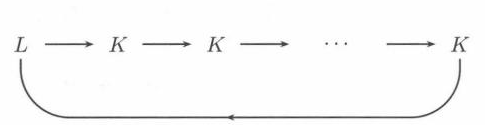
\includegraphics[width=.55\linewidth]{figures/upper/ch05/fig-5-3.png}

  图 5.3
\end{center}

对于所取的 $n$ 个区间应用引理 3，知道存在点 $x_0\in L$，满足
\begin{equation}
  f^n(x_0)=x_0,\qquad f^i(x_0)\in K,\ i=1,\ldots,n-1.
  \tag{5.8}
  \label{eq:5.8}
\end{equation}
若 $n$ 不是点 $x_0$ 的最小周期，则有 $p,1\le p<n$，使得 $f^p(x_0)=x_0$。由于这时 $f^p(x_0)\in K$，而 $x_0\in L$，因此与 (ii) 一样，只能有 $x_0=b$。但从条件 $n\ge3$ 和 $f^2(x_0)=f^2(b)=f(f(b))=f(c)=d\le a$ 可见 $f^2(x_0)\notin K$，与 (5.8) 相矛盾。

\begin{xexample}[5.6.4]
在区间 $[0,1]$ 上定义分段线性函数（其图像在图 5.4 上用粗黑的折线表示）：
\[
  f(x)=\begin{cases}
    x+\dfrac12,&0\le x\le\dfrac12,\\
    2(1-x),&\dfrac12<x\le1,
  \end{cases}
\]
则 $f$ 对一切 $n\in\NN_+$ 存在以 $n$ 为最小周期的周期轨。
\end{xexample}
\begin{xproof}
取 $a=0,b=\frac12,c=1$，则有 $f(0)=\frac12,f(\frac12)=1,f(1)=0$。因此从 Li-Yorke 第一定理知道结论成立。
\end{xproof}

\begin{xremark}
从图 5.4 可以清楚地看出，其中有周期 3 轨 $\{0,\frac12,1\}$，还有不动点 $\frac23$ 和由 $\{\frac13,\frac56\}$ 组成的周期 2 轨，其中周期 2 轨还特地用粗黑线的方框标出。图 5.4 中的箭头是按照第二章 §2.6 中介绍的蛛网工作法作出的。由于命题 5.6.1，在这样简单地由两段直线组成的图像上还存在无穷多个其周期取到一切正整数的周期轨，这完全超出了几何上的直观想象。在 [34] 发表之前很少有人能想到如此简单的函数会有如此奇妙的可能性。
\end{xremark}

\begin{center}
  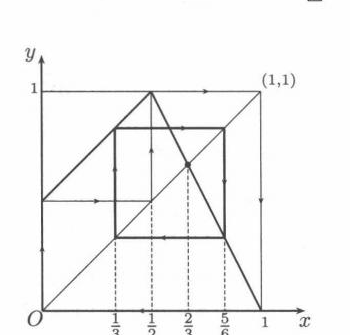
\includegraphics[width=.47\linewidth]{figures/upper/ch05/fig-5-4.png}

  图 5.4
\end{center}

现在介绍 [34] 中的第二个定理。虽然我们在这里并不证明，但了解一下它的内容也是很有意义的。这里的主要预备知识就是在第三章中的上、下极限。

\begin{xproposition}[5.6.2（Li-Yorke 第二定理）]
在与命题 5.6.1 相同的条件下，在区间 $I$ 中存在一个不可列集 $S$，使得以 $S$ 中的任何两点 $x,y\ (x\ne y)$ 为初值的迭代生成数列 $\{f^n(x)\}$ 和 $\{f^n(y)\}$ 具有以下三个性质：
\[
  \text{(1) }\varlimsup_{n\to\infty}|f^n(x)-f^n(y)|>0,
\]
\[
  \text{(2) }\varliminf_{n\to\infty}|f^n(x)-f^n(y)|=0,
\]
\[
  \text{(3) }\varlimsup_{n\to\infty}|f^n(x)-f^n(p)|>0,
\]
其中 $p$ 是 $f$ 的任何一个周期点。
\end{xproposition}

根据我们对上、下极限的理解，可以看出，由 $S$ 中任意两点出发的两个轨道（就是两个迭代生成数列）既会无限靠近，但又总会分离开。这样复杂的生态超出了过去的认识。因此就产生出 Li-Yorke 混沌的定义。

\begin{xdefinition}
设 $f$ 在区间 $I$ 上有定义，且有 $f(I)\subset I$。如果满足以下条件：
\begin{enumerate}
  \item $f$ 的周期点的最小周期无上界；
  \item 存在 $I$ 的不可列子集 $S$，对于 $S$ 中的任意两点 $x,y,x\ne y$，均有
  \[
    \text{(i) }\varlimsup_{n\to\infty}|f^n(x)-f^n(y)|>0,
    \qquad
    \text{(ii) }\varliminf_{n\to\infty}|f^n(x)-f^n(y)|=0,
  \]
\end{enumerate}
则称由 $f$ 迭代生成的动力系统为混沌。
\end{xdefinition}

应当指出，混沌在数学上目前存在各种不同的定义。而上述的 Li-Yorke 定义是在数学上第一个可操作的混沌定义。对混沌有兴趣的读者可以从 [21, 34, 38, 39] 中得到比这里丰富得多的材料。

\section{对于教学的建议}

\subsection{学习要点}

本章在极限理论的基础上介绍连续函数（以及单调函数）的基本性质。这是进入微分学（以及积分学）前的最后准备工作。

\begin{enumerate}
  \item 证明连续函数的基本定理和应用它们去解决各个问题不是一回事。实际上，由于这些基本定理反映了连续函数的深刻本质，因此它们将成为今后的重要工具。读者只有通过解题才能对如何运用这些工具获得直接的经验。
  \item 单调函数在数学分析中经常出现。本章对单调函数的基本性质作了小结。读者应当注意它们的基础是上一章中的命题 4.2.2。
  \item 以“周期 3 蕴涵混沌”为标题的 §5.6 可以作为课外活动材料。由于已有不少数学分析的新书收入了同样的（或更多的）材料，因此在 [39] 中作者的希望，即将迭代动力系统的材料放到初等课程中去教，正在变为现实。相信读者只要浏览一下就会看到这些最新发现与数学分析有密切关系。注意其中的第一个引理（即例题 5.6.1）已经成为数学分析教学中的基本题。
  \item \textbf{对习题课的建议}\quad 函数在某点的连续性概念的基础是极限概念，习题课老师可以把两者联系起来讲。可通过若干例题或课堂练习题来巩固这些概念。当然，复合函数的连续性（包括复合函数的极限存在性）是需要作一定训练的。例题 5.1.2、5.1.4 和 5.1.4 小节中的不少练习题等都是合适的材料。
\end{enumerate}

本章习题课重点在于连续函数的整体性质。从以往的教学经验看，学生对学习零点定理、介值定理、有界性定理和最值定理的兴趣比较大。这些定理也很直观。用本书所列举的材料已可组织起比较好的习题课。难点是一致连续性，应该安排为某次习题课的训练重点。本章的 §5.4 给出了训练的框架供参考。比如可分为一致连续的概念、一致连续的判断条件、一致连续的应用三个层次来复习。

\subsection{参考题}

\subsubsection*{第一组参考题}

\begin{xreferenceproblem}[1]
设非负函数 $f\in C[0,1]$，且 $f(0)=f(1)=0$。证明：对任一实数 $a\in(0,1)$，存在 $x_0\in[0,1]$，使得 $x_0+a\in[0,1]$，并满足要求 $f(x_0)=f(x_0+a)$。又问，如去掉函数 $f$ 非负的条件，则结论还成立否？
\end{xreferenceproblem}
\begin{xsolution}
固定 $a\in(0,1)$，在 $[0,1-a]$ 上定义
\[
 g(x)=f(x+a)-f(x).
\]
则 $g$ 连续。由 $f\ge0$ 及 $f(0)=f(1)=0$，
\[
 g(0)=f(a)\ge0,
 \qquad
 g(1-a)=f(1)-f(1-a)=-f(1-a)\le0.
\]
若其中一个等于 $0$ 已得结论；否则由零点存在定理存在 $x_0\in(0,1-a)$ 使 $g(x_0)=0$，即
\[
 f(x_0)=f(x_0+a).
\]

去掉非负条件后结论一般不成立。例如取
\[
 f(x)=\sin2\pi x,
 \qquad a=\frac34.
\]
则 $f(0)=f(1)=0$。对 $x\in[0,1/4]$，令 $t=2\pi x\in[0,\pi/2]$，有
\[
 f\left(x+\frac34\right)-f(x)
 =-\cos t-\sin t<0.
\]
因此不存在 $x\in[0,1/4]$ 使 $f(x)=f(x+3/4)$。
\end{xsolution}


\begin{xreferenceproblem}[2]
设 $f\in C[0,1],f(0)=f(1)$。证明：$\forall n\in\NN_+$，存在 $\xi$，使得 $f(\xi+1/n)=f(\xi)$。
\end{xreferenceproblem}
\begin{xsolution}
固定 $n\in\NN_+$。若 $n=1$，取 $\xi=0$ 即可。以下设 $n\ge2$，在 $[0,1-1/n]$ 上定义
\[
 g(x)=f\left(x+\frac1n\right)-f(x).
\]
若 $g$ 有零点即得结论。若无零点，由连续性知 $g$ 在整个区间恒正或恒负。但
\[
 \sum_{k=0}^{n-1}g\left(\frac{k}{n}\right)
 =\sum_{k=0}^{n-1}
 \left[f\left(\frac{k+1}{n}\right)-f\left(\frac{k}{n}\right)\right]
 =f(1)-f(0)=0,
\]
这与所有项同号矛盾。因此 $g$ 必有零点 $\xi$。
\end{xsolution}


\begin{xreferenceproblem}[3]
设 $f\in C[0,1],f([0,1])\subset[0,1]$。证明：$y=f(x)$ 的图像不仅与直线 $y=x$ 有交点，而且还与直线 $y=1-x$ 有交点。
\end{xreferenceproblem}
\begin{xsolution}
令
\[
 F(x)=f(x)-x.
\]
由 $f([0,1])\subset[0,1]$，
\[
 F(0)=f(0)\ge0,
 \qquad F(1)=f(1)-1\le0.
\]
故存在 $x_1\in[0,1]$ 使 $F(x_1)=0$，即图像与 $y=x$ 相交。

再令
\[
 G(x)=f(x)+x-1.
\]
则
\[
 G(0)=f(0)-1\le0,
 \qquad G(1)=f(1)\ge0.
\]
故存在 $x_2\in[0,1]$ 使 $G(x_2)=0$，即 $f(x_2)=1-x_2$，图像与 $y=1-x$ 相交。
\end{xsolution}


\begin{xreferenceproblem}[4]
设 $f\in C(0,+\infty)$，又对每个实数 $c$，方程 $f(x)=c$ 至多只有有限个实根。试分别给出极限 $\lim_{x\to+\infty}f(x)$ 及 $\lim_{x\to0^+}f(x)$ 存在的充分必要条件，并加以证明。
\end{xreferenceproblem}
\begin{xsolution}
这里把“极限存在”理解为存在有限实数极限。结论为：
\begin{enumerate}[label=(\arabic*)]
 \item $\lim_{x\to+\infty}f(x)$ 存在的充分必要条件是 $f$ 在某个尾区间 $[A,+\infty)$ 上有界；
 \item $\lim_{x\to0^+}f(x)$ 存在的充分必要条件是 $f$ 在某个 $(0,A]$ 上有界。
\end{enumerate}
必要性都由有限极限的局部有界性得到。先证第一条的充分性。

设 $f$ 在 $[A,+\infty)$ 上有界。若 $f(x)$ 在 $+\infty$ 处没有有限极限，则其尾部下极限与上极限满足
\[
 \alpha=\varliminf_{x\to+\infty}f(x)
 <
 \beta=\varlimsup_{x\to+\infty}f(x).
\]
取 $c\in(\alpha,\beta)$。于是无论把起点取得多大，后面总能找到函数值小于 $c$ 的点和函数值大于 $c$ 的点。可归纳取严格递增的点列
\[
 u_1<v_1<u_2<v_2<\cdots\to+\infty
\]
使 $f(u_j)<c<f(v_j)$（必要时交换两类点的次序）。由连续性，每个 $[u_j,v_j]$ 中都有一点 $z_j$ 满足 $f(z_j)=c$。这使方程 $f(x)=c$ 有无限多个实根，与题设矛盾。因此 $\alpha=\beta$，有限极限存在。

再证第二条的充分性。若 $f$ 在 $(0,A]$ 上有界，令
\[
 h(t)=f(1/t),
 \qquad t\in[1/A,+\infty).
\]
则 $h$ 连续且有界；并且对每个 $c\in\RR$，方程 $h(t)=c$ 的根数不超过方程 $f(x)=c$ 的根数，因而也是有限的。由刚证得的第一条，$\lim_{t\to+\infty}h(t)$ 存在。令 $x=1/t$，即得 $\lim_{x\to0^+}f(x)$ 存在。
\end{xsolution}


\begin{xreferenceproblem}[5]
设 $f$ 在 $(-\infty,+\infty)$ 上有定义，对于任意 $x,y$，满足 $|f(x)-f(y)|\le k|x-y|\ (0<k<1)$。证明：
  \begin{enumerate}[label=(\arabic*)]
    \item 函数 $kx-f(x)$ 单调增加；
    \item 存在唯一的 $\xi$，使 $f(\xi)=\xi$。
  \end{enumerate}
\end{xreferenceproblem}
\begin{xsolution}
\begin{enumerate}[label=(\arabic*)]
 \item 对 $x<y$，由题设
 \[
  f(y)-f(x)\le |f(y)-f(x)|\le k(y-x),
 \]
 故
 \[
  [ky-f(y)]-[kx-f(x)]
  =k(y-x)-[f(y)-f(x)]\ge0.
 \]
 因此 $kx-f(x)$ 单调增加。

 \item 令 $F(x)=f(x)-x$。对 $x<y$，
 \[
  F(y)-F(x)=f(y)-f(x)-(y-x)
  \le -(1-k)(y-x)<0,
 \]
 所以 $F$ 严格减少，零点至多一个。

 又由 Lipschitz 条件
 \[
  f(x)\le f(0)+kx\quad(x>0),
 \]
 从而
 \[
  F(x)\le f(0)-(1-k)x\to-\infty
  \qquad(x\to+\infty).
 \]
 对 $x<0$，
 \[
  f(x)\ge f(0)-k|x|=f(0)+kx,
 \]
 故
 \[
  F(x)\ge f(0)+(k-1)x\to+\infty
  \qquad(x\to-\infty).
 \]
 $F$ 连续，因此由零点存在定理有且仅有一个 $\xi$ 满足 $F(\xi)=0$，即 $f(\xi)=\xi$。
\end{enumerate}
\end{xsolution}


\begin{xreferenceproblem}[6]
设 $f_n(x)=x^n+x,n\in\NN_+$。
  \begin{enumerate}[label=(\arabic*)]
    \item 证明：对每个 $n>1$，方程 $f_n(x)=1$ 在 $(1/2,1)$ 内有且仅有一个根；
    \item 证明：由 $c_n\in(1/2,1)$ 是 $f_n(x)=1$ 的根，则存在 $\lim_{n\to\infty}c_n$。试求出极限值。
  \end{enumerate}
\end{xreferenceproblem}
\begin{xsolution}
\begin{enumerate}[label=(\arabic*)]
 \item 对 $n>1$，函数 $f_n(x)=x^n+x$ 在 $(0,+\infty)$ 上严格增加。并且
 \[
  f_n(1/2)=2^{-n}+\frac12<1,
  \qquad f_n(1)=2>1.
 \]
 由零点存在定理，$f_n(x)=1$ 在 $(1/2,1)$ 内有根；严格增加性又保证根唯一。

 \item 记唯一根为 $c_n$。因 $0<c_n<1$，有
 \[
  f_{n+1}(c_n)=c_n^{n+1}+c_n<c_n^n+c_n=1.
 \]
 而 $f_{n+1}$ 严格增加，所以
 \[
  c_{n+1}>c_n.
 \]
 因此 $\{c_n\}$ 单调增加且以 $1$ 为上界，故存在极限 $L\le1$。若 $L<1$，取 $q$ 使 $L<q<1$，则充分大时 $c_n<q$，从而 $c_n^n\le q^n\to0$。由方程
 \[
  c_n^n=1-c_n
 \]
 令 $n\to\infty$ 得 $0=1-L$，矛盾。因此
 \[
  \boxed{\lim_{n\to\infty}c_n=1}.
 \]
\end{enumerate}
\end{xsolution}


\begin{xreferenceproblem}[7]
设对每个正整数 $n$，数集 $A_n\subset[0,1]$ 是有限集，而且 $A_i\cap A_j=\varnothing,\ \forall i,j\in\NN_+,i\ne j$。定义函数
  \[
    f(x)=\begin{cases}
      \dfrac1n,&\text{若 }x\in A_n,\\
      0,&\text{若 }x\in[0,1]\text{ 但不在任何 }A_n\text{ 中}.
    \end{cases}
  \]
  对每个 $a\in[0,1]$，求 $\lim_{x\to a}f(x)$。
\end{xreferenceproblem}
\begin{xsolution}
固定 $a\in[0,1]$ 与 $\varepsilon>0$。取 $N$ 使 $1/N<\varepsilon$。有限并
\[
 E=A_1\cup\cdots\cup A_N
\]
仍为有限集。可取 $\delta>0$，使去心邻域
\[
 0<|x-a|<\delta
\]
中没有 $E$ 的点。于是这样的 $x$ 若属于某个 $A_n$，必有 $n>N$，从而
\[
 |f(x)|=\frac1n<\frac1N<\varepsilon;
\]
若不属于任何 $A_n$，则 $f(x)=0$。所以
\[
 \boxed{\lim_{x\to a}f(x)=0}
\]
对每个 $a\in[0,1]$ 都成立。
\end{xsolution}


\begin{xreferenceproblem}[8]
设函数 $f$ 在区间 $I$ 内只有可去间断点。定义 $g(x)=\lim_{t\to x}f(t),x\in I$，证明：$g\in C(I)$。
\end{xreferenceproblem}
\begin{xsolution}
记
\[
 g(x)=\lim_{t\to x}f(t).
\]
固定 $x_0\in I$。给定 $\varepsilon>0$，由 $f(t)\to g(x_0)$ 当 $t\to x_0$，可取 $\delta>0$，使
\[
 0<|t-x_0|<\delta
 \quad\Longrightarrow\quad
 |f(t)-g(x_0)|<\frac\varepsilon2.
\]
若 $|x-x_0|<\delta/2$，则取 $t\to x$ 且 $t\ne x$ 时，可令 $t$ 同时落在 $O_\delta(x_0)$ 内。于是
\[
 |f(t)-g(x_0)|<\frac\varepsilon2.
\]
令 $t\to x$，得到
\[
 |g(x)-g(x_0)|\le\frac\varepsilon2<\varepsilon.
\]
所以 $g$ 在 $x_0$ 连续。$x_0$ 任意，故 $g\in C(I)$。
\end{xsolution}


\begin{xreferenceproblem}[9]
证明：若函数 $f$ 在区间 $[0,+\infty)$ 上连续且有界，则对每个给定的 $\lambda$，存在一个数列 $\{x_n\}$ 满足要求：(1) $\lim_{n\to\infty}x_n=+\infty$；(2) $\lim_{n\to\infty}[f(x_n+\lambda)-f(x_n)]=0$。
\end{xreferenceproblem}
\begin{xsolution}
若 $\lambda=0$，任取 $x_n\to+\infty$ 即可。先设 $\lambda>0$。对于 $\lambda<0$，令 $\mu=-\lambda>0$；若已对 $\mu$ 找到 $y_n\to+\infty$ 使 $f(y_n+\mu)-f(y_n)\to0$，再取 $x_n=y_n+\mu$，便有
\[
 f(x_n+\lambda)-f(x_n)=f(y_n)-f(y_n+\mu)\to0.
\]
因此只需证明 $\lambda>0$ 的情形。

令
\[
 g(x)=f(x+\lambda)-f(x).
\]
若结论不成立，则存在 $\varepsilon_0>0$ 和 $M$，使对所有 $x>M$ 都有
\[
 |g(x)|\ge\varepsilon_0.
\]
因为 $g$ 连续且在连通区间 $(M,+\infty)$ 上不取 $0$，它在该区间恒正或恒负。若 $g(x)\ge\varepsilon_0$，则对固定 $x>M$，
\[
 f(x+n\lambda)-f(x)
 =\sum_{j=0}^{n-1}g(x+j\lambda)
 \ge n\varepsilon_0,
\]
与 $f$ 有界矛盾；若 $g\le-\varepsilon_0$ 同理矛盾。因此对每个 $n$ 都能取 $x_n>n$ 使
\[
 |f(x_n+\lambda)-f(x_n)|<\frac1n.
\]
于是 $x_n\to+\infty$ 且所要求的差趋于 $0$。
\end{xsolution}


\begin{xreferenceproblem}[10]
设函数 $f$ 在区间 $I$ 上满足带指数的 Lipschitz 条件，即存在 $M>0,\alpha>0$，使得当 $x,y\in I$ 时，成立 $|f(x)-f(y)|\le M|x-y|^\alpha$。证明：若 $\alpha>1$，则 $f$ 在 $I$ 上是常值函数。
\end{xreferenceproblem}
\begin{xsolution}
任取 $x<y$，把 $[x,y]$ 等分为 $n$ 段，分点记为
\[
 x=x_0<x_1<\cdots<x_n=y,
 \qquad x_j-x_{j-1}=\frac{y-x}{n}.
\]
由题设及三角不等式，
\[
 \begin{aligned}
 |f(y)-f(x)|
 &\le\sum_{j=1}^n|f(x_j)-f(x_{j-1})|\\
 &\le nM\left(\frac{y-x}{n}\right)^\alpha
 =M(y-x)^\alpha n^{1-\alpha}.
 \end{aligned}
\]
若 $\alpha>1$，令 $n\to\infty$，右端趋于 $0$，故 $f(y)=f(x)$。任意两点函数值相同，所以 $f$ 为常值函数。
\end{xsolution}


\begin{xreferenceproblem}[11]
举出一个函数 $f$，它的定义域为 $[0,1]$，处处不连续，但它的值域为区间。
\end{xreferenceproblem}
\begin{xsolution}
先定义
\[
 h(x)=\begin{cases}
 x,&x\in\QQ,\\
 1-x,&x\notin\QQ,
 \end{cases}
 \qquad 0\le x\le1.
\]
$h$ 的值域恰为 $[0,1]$，并且除 $x=1/2$ 外处处不连续；在 $1/2$ 处两类趋近的函数值都趋于 $1/2$。

现只交换 $h$ 在 $0$ 与 $1/2$ 的两个函数值，定义
\[
 f(0)=\frac12,
 \qquad f\left(\frac12\right)=0,
\]
其余点令 $f(x)=h(x)$。交换两个值不改变值域，所以 $f([0,1])=[0,1]$。对 $x_0\ne1/2$，有理、无理数列趋于 $x_0$ 时函数值分别趋于 $x_0$ 与 $1-x_0$，两者不同，故不连续；在 $x_0=1/2$，极限为 $1/2$ 而函数值为 $0$，也不连续。因此 $f$ 处处不连续而值域为区间。
\end{xsolution}


\begin{xreferenceproblem}[12]
若 $f\in C[a,b]$，证明：对每个给定的 $\varepsilon>0$，存在区间 $[a,b]$ 上的分段线性函数 $L(x)$，使得 $|f(x)-L(x)|<\varepsilon$ 在区间 $[a,b]$ 上处处成立。
\end{xreferenceproblem}
\begin{xsolution}
由 Cantor 定理，$f$ 在 $[a,b]$ 上一致连续。给定 $\varepsilon>0$，取 $\delta>0$，使
\[
 |x-y|<\delta
 \quad\Longrightarrow\quad
 |f(x)-f(y)|<\varepsilon.
\]
取分点
\[
 a=x_0<x_1<\cdots<x_N=b
\]
使每段长度小于 $\delta$，并令 $L$ 在每个 $[x_{j-1},x_j]$ 上为连接
\[
 (x_{j-1},f(x_{j-1})),\qquad (x_j,f(x_j))
\]
的线性函数。若 $x\in[x_{j-1},x_j]$，则存在 $0\le\theta\le1$ 使
\[
 L(x)=(1-\theta)f(x_{j-1})+\theta f(x_j).
\]
于是
\[
 \begin{aligned}
 |f(x)-L(x)|
 &\le(1-\theta)|f(x)-f(x_{j-1})|
   +\theta|f(x)-f(x_j)|\\
 &<\varepsilon.
 \end{aligned}
\]
故得到所要求的分段线性函数。
\end{xsolution}


\begin{xreferenceproblem}[13]
设 $f\in C(-\infty,+\infty)$，且 $\lim_{x\to\infty}f(f(x))=\infty$，证明：$\lim_{x\to\infty}f(x)=\infty$。
\end{xreferenceproblem}
\begin{xsolution}
这里无符号的 $\infty$ 表示无穷大，即题设为
\[
 |f(f(x))|\to+\infty,
\]
所需证明的结论为 $|f(x)|\to+\infty$。

反设结论不成立，则存在常数 $M>0$ 和数列 $x_n\to+\infty$，使
\[
 |f(x_n)|\le M,
 \qquad n\in\NN_+.
\]
由于 $f$ 在闭区间 $[-M,M]$ 上连续，存在 $K>0$ 使
\[
 |f(y)|\le K,
 \qquad |y|\le M.
\]
于是
\[
 |f(f(x_n))|\le K,
\]
这与 $|f(f(x))|\to+\infty$ 矛盾。因此
\[
 |f(x)|\to+\infty.
\]
\end{xsolution}


\begin{xreferenceproblem}[14]
设 $f\in C(-\infty,+\infty)$，且存在 $k>0$，使得对任意 $x_1,x_2\in\RR$，成立 $|f(x_1)-f(x_2)|\ge k|x_1-x_2|$。证明：$f$ 严格单调且值域为 $(-\infty,+\infty)$。
\end{xreferenceproblem}
\begin{xsolution}
题设立即给出一一性：若 $f(x_1)=f(x_2)$，则
\[
 0\ge k|x_1-x_2|,
\]
故 $x_1=x_2$。连续的一一函数在区间 $\RR$ 上严格单调。

又取 $x_2=0$ 得
\[
 |f(x)-f(0)|\ge k|x|,
\]
从而
\[
 |f(x)|\ge k|x|-|f(0)|\to+\infty
 \qquad(|x|\to\infty).
\]
若 $f$ 严格增加，则不可能在 $+\infty$ 方向趋于 $-\infty$，也不可能在 $-\infty$ 方向趋于 $+\infty$，故
\[
 \lim_{x\to-\infty}f(x)=-\infty,
 \qquad
 \lim_{x\to+\infty}f(x)=+\infty.
\]
若严格减少则两式符号相反。两种情况下由介值定理都得到
\[
 f(\RR)=\RR.
\]
\end{xsolution}


\begin{xreferenceproblem}[15]
证明：不等于常数的连续周期函数一定有最小正周期。又问：如果将连续性条件去掉，结论还能成立否？\footnote{注意：非常值周期函数若有一个连续点，则必有最小周期。见 [59] 第一册 79 页命题 1.5。}
\end{xreferenceproblem}
\begin{xsolution}
设 $P$ 为 $f$ 的所有正周期组成的集合。先证
\[
 \tau=\inf P>0.
\]
若不然，可取周期 $T_n\downarrow0$。任取 $x,y\in\RR$，对每个 $n$ 取整数 $m_n$，使
\[
 |x+m_nT_n-y|\le\frac{T_n}{2}.
\]
由周期性 $f(x+m_nT_n)=f(x)$，而 $x+m_nT_n\to y$。连续性给出
\[
 f(x)=\lim_{n\to\infty}f(x+m_nT_n)=f(y).
\]
这会使 $f$ 成为常值函数，与题设矛盾。因此 $\tau>0$。

按下确界定义可取 $T_n\in P$ 使 $T_n\to\tau$。对任意 $x$，
\[
 f(x+\tau)
 =\lim_{n\to\infty}f(x+T_n)
 =f(x),
\]
故 $\tau$ 本身也是周期。由定义它就是最小正周期。

若去掉连续性，结论不成立。Dirichlet 函数 $D$ 的每个正有理数都是周期，因为平移有理数不改变一个数的有理性；但正有理数没有最小元，所以 $D$ 没有最小正周期。
\end{xsolution}


\begin{xreferenceproblem}[16]
设函数 $f$ 在区间 $[a,+\infty)$ 上满足 Lipschitz 条件，其中 $a>0$。证明：$f(x)/x$ 在 $[a,+\infty)$ 上一致连续。
\end{xreferenceproblem}
\begin{xsolution}
设 $f$ 的 Lipschitz 常数为 $L$。对 $x\ge a$，
\[
 |f(x)|\le |f(a)|+L(x-a)\le Lx+B,
 \qquad B=|f(a)|+La.
\]
令 $g(x)=f(x)/x$。对 $x,y\ge a$，
\[
 \begin{aligned}
 |g(x)-g(y)|
 &\le\frac{|f(x)-f(y)|}{x}
 +|f(y)|\left|\frac1x-\frac1y\right|\\
 &\le\frac{L}{a}|x-y|
 +(Ly+B)\frac{|x-y|}{xy}\\
 &\le\left[\frac{L}{a}+\frac{L+B/a}{a}\right]|x-y|.
 \end{aligned}
\]
所以 $g$ 本身满足 Lipschitz 条件，从而在 $[a,+\infty)$ 上一致连续。
\end{xsolution}


\begin{xreferenceproblem}[17]
证明：函数 $f$ 在区间 $I$ 上一致连续的充分必要条件是：对任何满足条件 $\lim_{n\to\infty}(x_n-y_n)=0$ 的 $\{x_n\}\subset I$ 和 $\{y_n\}\subset I$，都有 $\lim_{n\to\infty}[f(x_n)-f(y_n)]=0$。
\end{xreferenceproblem}
\begin{xsolution}
若 $f$ 一致连续，而 $x_n-y_n\to0$，则给定 $\varepsilon>0$，取一致连续性中的 $\delta$。充分大时 $|x_n-y_n|<\delta$，于是
\[
 |f(x_n)-f(y_n)|<\varepsilon,
\]
故差趋于 $0$。

反之，若 $f$ 不一致连续，则存在 $\varepsilon_0>0$，对每个 $n$ 可取 $x_n,y_n\in I$ 使
\[
 |x_n-y_n|<\frac1n,
 \qquad
 |f(x_n)-f(y_n)|\ge\varepsilon_0.
\]
于是 $x_n-y_n\to0$，但函数值之差不趋于 $0$，与题设的序列条件矛盾。因此该条件也充分。
\end{xsolution}


\begin{xreferenceproblem}[18]
证明：函数 $f$ 在有界区间 $I$ 上一致连续的充分必要条件是：当 $\{x_n\}$ 为基本数列时，$\{f(x_n)\}$ 也一定是基本数列。
\end{xreferenceproblem}
\begin{xsolution}
若 $f$ 一致连续，设 $\{x_n\}\subset I$ 为基本数列。给定 $\varepsilon>0$，取一致连续性中的 $\delta$；再由 $\{x_n\}$ 为基本数列，取 $N$ 使 $m,n>N$ 时 $|x_m-x_n|<\delta$。于是
\[
 |f(x_m)-f(x_n)|<\varepsilon,
\]
故 $\{f(x_n)\}$ 也是基本数列。

反之，若 $f$ 不一致连续，则存在 $\varepsilon_0>0$ 以及 $x_n,y_n\in I$，使
\[
 |x_n-y_n|<\frac1n,
 \qquad |f(x_n)-f(y_n)|\ge\varepsilon_0.
\]
因 $I$ 有界，$\{x_n\}$ 有收敛子列 $x_{n_k}\to\xi$；相应地 $y_{n_k}\to\xi$。交错排列
\[
 z_{2k-1}=x_{n_k},
 \qquad z_{2k}=y_{n_k},
 \qquad k\in\NN_+,
\]
得到一个 $I$ 中的基本数列。但
\[
 |f(z_{2k-1})-f(z_{2k})|
 \ge\varepsilon_0,
\]
所以 $\{f(z_n)\}$ 不是基本数列，矛盾。故 $f$ 必一致连续。
\end{xsolution}


\begin{xreferenceproblem}[19]
设函数 $f$ 在区间 $[0,+\infty)$ 上一致连续，且对任何 $x\in[0,1]$ 有 $\lim_{n\to\infty}f(x+n)=0$。证明：$\lim_{x\to+\infty}f(x)=0$。
\end{xreferenceproblem}
\begin{xsolution}
给定 $\varepsilon>0$。由 $f$ 在 $[0,+\infty)$ 上一致连续，存在 $\delta>0$，使
\[
 |u-v|<\delta
 \Longrightarrow
 |f(u)-f(v)|<\frac\varepsilon2.
\]
在 $[0,1]$ 中选有限个点 $t_1,\ldots,t_m$，使每个 $t\in[0,1]$ 与某个 $t_j$ 的距离小于 $\delta$。对每个 $j$，由
\[
 f(t_j+n)\to0
\]
可取同一个足够大的整数 $N$，使当 $n\ge N$ 时
\[
 |f(t_j+n)|<\frac\varepsilon2,
 \qquad j=1,\ldots,m.
\]
任取充分大的 $x$，写成 $x=n+t$，其中 $n\in\NN$、$t\in[0,1)$，并令 $n\ge N$。选 $t_j$ 使 $|t-t_j|<\delta$，则
\[
 |f(x)|
 \le |f(n+t)-f(n+t_j)|+|f(n+t_j)|
 <\varepsilon.
\]
所以 $f(x)\to0$ 当 $x\to+\infty$。
\end{xsolution}


\begin{xreferenceproblem}[20]
设 $f$ 在 $(-\infty,+\infty)$ 上一致连续，证明：存在非负常数 $a$ 和 $b$，使得成立 $|f(x)|\le a|x|+b$。
\end{xreferenceproblem}
\begin{xsolution}
由一致连续性，对 $\varepsilon=1$ 可取 $\delta>0$，使
\[
 |u-v|<\delta
 \Longrightarrow
 |f(u)-f(v)|<1.
\]
固定 $x\in\RR$。把从 $0$ 到 $x$ 的线段分成 $N$ 段，使每段长度小于 $\delta$，并可取
\[
 N\le\frac{2|x|}{\delta}+1.
\]
沿分点逐段使用三角不等式，得到
\[
 |f(x)-f(0)|<N
 \le\frac{2|x|}{\delta}+1.
\]
因此
\[
 |f(x)|
 \le \frac{2}{\delta}|x|+|f(0)|+1.
\]
取
\[
 a=\frac2\delta\ge0,
 \qquad b=|f(0)|+1\ge0,
\]
即得所需估计。
\end{xsolution}


\subsubsection*{第二组参考题}

\begin{xreferenceproblem}[1]
用连续函数的零点存在定理解决以下“实际问题”：
  \begin{enumerate}[label=(\arabic*)]
    \item 一个煎饼，不论形状如何，必可切一刀，使面积二等分；
    \item 两个煎饼，不论形状如何，相对位置如何，必可切一刀，使它们的面积同时二等分（双煎饼定理）；
    \item 三个煎饼，不论形状如何，相对位置如何，能否切一刀，使它们的面积同时二等分？
    \item 一个煎饼，不论形状如何，是否能以相互垂直的方式切两刀，使面积四等分？
    \item 某短跑运动员用 $10\,\mathrm{s}$ 跑完 $100\,\mathrm{m}$。证明：其中至少有一段长为 $10\,\mathrm{m}$ 的路程恰用 $1\,\mathrm{s}$ 完成；
    \item 四只脚的方台在不平整的地上可能会摇晃。但如适当转动的话，一定能找到使它不摇晃的位置（若做实验会很有趣）；
    \item 给定平面上的一条光滑的封闭曲线，能否作一个包含这条闭曲线的正方形，并且它的四边都与曲线相切（方镜框定理）？
  \end{enumerate}

  （本题中出现的许多概念，包括区域、边界、面积、光滑曲线和相切等，在今后的教学中将会得到严格的数学处理。但是目前可以采取朴素的观点来对待题中的条件，因为在所有这些题中，主要的工具只是零点存在定理，再加上你的想象力。）
\end{xreferenceproblem}
\begin{xsolution}
下面都只使用题目允许的朴素几何观点，并把面积随直线位置、方向连续变化这一事实作为连续性工具。

\begin{enumerate}[label=(\arabic*)]
 \item 固定一个方向，让一条与该方向垂直的直线从煎饼一侧平行移动到另一侧。记直线某一侧的面积减去另一侧的面积为 $F(t)$。当直线在煎饼一侧之外时，$F$ 的符号为负；移到另一侧之外时，符号为正。$F(t)$ 连续，故由零点存在定理存在位置使 $F(t)=0$，即一刀把面积二等分。

 \item 对每个方向 $\theta$，先取一条方向为 $\theta$ 的直线 $L_\theta$，使第一个煎饼被二等分。若这样的直线不唯一，可在所有二等分位置组成的区间中取中点，从而使选择随 $\theta$ 连续。令
 \[
  H(\theta)=\text{第二个煎饼在 }L_\theta\text{ 两侧的面积差}.
 \]
 当方向反转为 $\theta+\pi$ 时，同一条无向直线的两侧互换，故
 \[
  H(\theta+\pi)=-H(\theta).
 \]
 $H$ 连续，因此在 $[\theta,\theta+\pi]$ 中必有 $H=0$ 的方向。相应直线同时二等分两个煎饼。

 \item 一般不能。取三个互不共线的圆盘。任何把一个圆盘面积二等分的直线必须经过圆心，因此若一条直线同时二等分三个圆盘，它必须同时经过三个不共线圆心，这是不可能的。

 \item 可以。对每个方向 $\theta$，分别取方向为 $\theta$ 和 $\theta+\pi/2$ 的两条面积二等分线 $L_\theta,M_\theta$；若某方向的二等分线不唯一，就取所有二等分位置组成区间的中点。这样两条线可随 $\theta$ 连续选取。它们把平面分成四个象限，按逆时针记煎饼落在四个象限中的面积为 $A_1,A_2,A_3,A_4$。因为 $L_\theta$、$M_\theta$ 各自都二等分总面积，
 \[
  A_1+A_2=A_3+A_4,
  \qquad
  A_2+A_3=A_4+A_1.
 \]
 因而 $A_1=A_3$、$A_2=A_4$。令
 \[
  G(\theta)=A_1-A_2.
 \]
 当 $\theta$ 增加 $\pi/2$ 时，两条互相垂直的二等分线交换角色，四个象限循环移动一格，因此
 \[
  G\left(\theta+\frac\pi2\right)=A_2-A_3=-G(\theta).
 \]
 面积对方向连续，所以 $G$ 连续。由零点存在定理存在 $\theta_0$ 使 $G(\theta_0)=0$。这时 $A_1=A_2=A_3=A_4$，而四者之和为总面积，故每块面积均为总面积的 $1/4$。

 \item 设运动员在时刻 $t$ 已跑过的路程为 $s(t)$。则 $s$ 连续，$s(0)=0,s(10)=100$。在 $[0,9]$ 上令
 \[
  g(t)=s(t+1)-s(t)-10.
 \]
 若不存在 $g(t)=0$，因 $g$ 连续，它必在整个 $[0,9]$ 上恒正或恒负。但
 \[
  \sum_{k=0}^{9}g(k)
  =s(10)-s(0)-100=0,
 \]
 与所有项同号矛盾。所以存在 $t_0\in[0,9]$ 使
 \[
  s(t_0+1)-s(t_0)=10,
 \]
 即有一段 $10\,\mathrm m$ 的路程恰用 $1\,\mathrm s$ 完成。

 \item 固定方台中心位置，只让方台绕竖直轴转动。把一条对角线两端两只脚的“着地高度和”减去另一条对角线两端两只脚的“着地高度和”，记为 $H(\theta)$。地面高度连续时，$H$ 随转角连续。转过 $\pi/2$ 后两条对角线交换，故
 \[
  H\left(\theta+\frac\pi2\right)=-H(\theta).
 \]
 因而某个角度有 $H=0$。此时四个脚点共面，刚性方台四脚可同时接触地面，于是不再摇晃。

 \item 对每个方向 $\theta$，作两条方向为 $\theta$ 的平行支撑线夹住闭曲线，记两线距离即该方向的宽度为 $w(\theta)$。光滑闭曲线的支撑线与曲线相切，且 $w(\theta)$ 连续。考虑
 \[
  H(\theta)=w(\theta)-w\left(\theta+\frac\pi2\right).
 \]
 则
 \[
  H\left(\theta+\frac\pi2\right)
  =-H(\theta).
 \]
 故存在 $\theta_0$ 使 $H(\theta_0)=0$。于是方向 $\theta_0$ 与垂直方向的两对支撑线距离相等，四条支撑线围成一个正方形，并且四边都与曲线相切。
\end{enumerate}
\end{xsolution}


\begin{xreferenceproblem}[2]
设函数 $f$ 在区间 $[0,n]$ 上连续，且有 $f(0)=f(n)$，其中 $n$ 是一个正整数。证明：至少有 $n$ 对不同的 $(x,y)$，使得 $f(x)=f(y)$，同时 $x-y$ 为非零整数。
\end{xreferenceproblem}
\begin{xsolution}
把 $f$ 以周期 $n$ 连续延拓到 $\RR$，记延拓仍为 $f$。对整数 $k=1,\ldots,n-1$ 定义
\[
 h_k(x)=f(x+k)-f(x).
\]
令 $r=n/\gcd(n,k)$。由于在模 $n$ 意义下
\[
 x,x+k,\ldots,x+(r-1)k
\]
构成一个循环，有
\[
 \sum_{j=0}^{r-1}h_k(x+jk)=0.
\]
因此若 $h_k$ 不恒为零，它必取正值和负值，故在一个周期圆周上至少有两个零点；若恒为零，则零点当然更多。

现在只取
\[
 1\le k<\frac n2.
\]
对每个这样的 $k$，至少可得到两个不同的无序点对 $\{x,x+k\}$（模 $n$），其两点函数值相同。不同 $k$ 对应的圆周短距离不同，所以这些点对互不相同。若 $n$ 为偶数，再取 $k=n/2$。这时
\[
 h_{n/2}\left(x+\frac n2\right)=-h_{n/2}(x),
\]
故至少得到一个这样的点对。

于是当 $n$ 为奇数时得到
\[
 2\cdot\frac{n-1}{2}=n-1
\]
对；当 $n$ 为偶数时得到
\[
 2\left(\frac n2-1\right)+1=n-1
\]
对。把圆周上的各点取在 $[0,n)$ 的代表元中，每一对的两个代表元之差为非零整数。最后再加入端点对 $(0,n)$，由 $f(0)=f(n)$，总共至少得到 $n$ 对不同的 $(x,y)$。
\end{xsolution}


\begin{xreferenceproblem}[3]
设函数 $f$ 在 $[a,b]$ 上定义，且处处有极限。证明：
  \begin{enumerate}[label=(\arabic*)]
    \item 对每个 $\varepsilon>0$，在 $[a,b]$ 中使 $|\lim_{t\to x}f(t)-f(x)|>\varepsilon$ 的点至多只有有限个；
    \item $f$ 在 $[a,b]$ 中至多只有可列个间断点。
  \end{enumerate}
\end{xreferenceproblem}
\begin{xsolution}
记
\[
 L(x)=\lim_{t\to x}f(t).
\]
由第一组参考题 8 的结论，$L\in C[a,b]$。

\begin{enumerate}[label=(\arabic*)]
 \item 固定 $\varepsilon>0$。若满足
 \[
  |L(x)-f(x)|>\varepsilon
 \]
 的点有无限多个，则可取互异点列 $x_n$，由闭区间的凝聚性再取子列（仍记为 $x_n$）使 $x_n\to x_0\in[a,b]$。

 因为 $f$ 在 $x_0$ 处有极限，且 $x_n\ne x_0$，所以
 \[
  f(x_n)\to L(x_0).
 \]
 又因 $L$ 连续，
 \[
  L(x_n)\to L(x_0).
 \]
 因此
 \[
  |L(x_n)-f(x_n)|\to0,
 \]
 与它始终大于 $\varepsilon$ 矛盾。故这样的点至多有限个。

 \item 点 $x$ 是可去间断点当且仅当 $f(x)\ne L(x)$。于是全部间断点集合为
 \[
  \bigcup_{m=1}^\infty
  \left\{x\in[a,b]:|L(x)-f(x)|>\frac1m\right\}.
 \]
 由 (1)，每个括号中的集合有限，故该并集至多可列。
\end{enumerate}
\end{xsolution}


\begin{xreferenceproblem}[4]
证明：区间上的函数不可能以区间的每个点为它的可去间断点。
\end{xreferenceproblem}
\begin{xsolution}
若区间 $I$ 的每一点都是 $f$ 的可去间断点，记
\[
 L(x)=\lim_{t\to x}f(t).
\]
对任意有界闭子区间 $[c,d]\subset I$，由上一题，集合
\[
 E_m=\left\{x\in[c,d]:|L(x)-f(x)|>\frac1m\right\}
\]
都是有限集。而每一点都是可去间断点，故 $f(x)\ne L(x)$，从而
\[
 [c,d]=\bigcup_{m=1}^\infty E_m.
\]
右边是可列集，左边却不可列，矛盾。因此不存在这样的函数。
\end{xsolution}


\begin{xreferenceproblem}[5]
是否存在定义于 $(-\infty,+\infty)$ 上的连续函数 $f$，使对于每个 $c\in\RR$，
  \begin{enumerate}[label=(\arabic*)]
    \item 方程 $f(x)=c$ 都恰有两个解？
    \item 方程 $f(x)=c$ 都恰有三个解？
  \end{enumerate}
\end{xreferenceproblem}
\begin{xsolution}
\begin{enumerate}[label=(\arabic*)]
 \item 不存在。反设连续函数 $f\colon\RR\to\RR$ 对每个 $c$ 恰有两个原像。取某个 $c$，设两个原像为 $a<b$。在 $(a,b)$ 上 $f-c$ 不取零值，故恒正或恒负。

 若 $f>c$ 于 $(a,b)$，在 $[a,b]$ 上取最大值 $M>c$。取 $d\in(c,M)$。由介值定理，方程 $f(x)=d$ 在 $(a,b)$ 至少有两个解，因此按题设恰有这两个解。若在 $(-\infty,a)$ 或 $(b,+\infty)$ 中某处有 $f>d$，从该点到 $a$ 或 $b$ 再用介值定理会产生第三个 $d$ 的原像，矛盾。因此区间外有 $f<d$，而区间内 $f\le M$，所以 $f$ 在 $\RR$ 上有上界。这与每个任意大的实数都应成为某个函数值矛盾。若 $f<c$ 于 $(a,b)$，同理得到全局下界，也矛盾。

 \item 存在。定义连续分段线性函数 $F$，使对每个 $m\in\ZZ$，
 \[
  F(3m)=m,
  \quad F(3m+1)=m+1,
  \quad F(3m+2)=m,
  \quad F(3m+3)=m+1,
 \]
 并在相邻整数间线性插值。若 $c\in(m,m+1)$，水平线 $y=c$ 恰与区间
 \[
  (3m,3m+1),\quad(3m+1,3m+2),\quad(3m+2,3m+3)
 \]
 上的三条线段各交一次，所以恰有三个解。若 $c=m$ 是整数，则原像恰为
 \[
  3m-2,\quad3m,\quad3m+2,
 \]
 仍恰有三个。因此所求函数存在。
\end{enumerate}
\end{xsolution}


\begin{xreferenceproblem}[6]
设 $n$ 为正整数，求满足函数方程 $f(x+y^n)=f(x)+(f(y))^n\ (x,y\in\RR)$ 的所有解。
\end{xreferenceproblem}
\begin{xsolution}
方程为
\[
 f(x+y^n)=f(x)+(f(y))^n,
 \qquad x,y\in\RR.
\]
令 $y=0$ 得 $f(0)=0$；再令 $x=0$ 得
\[
 f(y^n)=f(y)^n.
\]
于是
\[
 f(x+y^n)=f(x)+f(y^n).
\]

若 $n$ 为奇数，则 $y^n$ 遍历 $\RR$，故 $f$ 是加法函数。若 $n$ 为偶数，则上式先给出
\[
 f(x+t)=f(x)+f(t),\qquad t\ge0.
\]
取 $x=-t$ 得 $f(-t)=-f(t)$，于是同样可推广到任意实数增量，故 $f$ 仍是加法函数。

当 $n=1$ 时，原方程正是 Cauchy 加法方程，因此所有加法函数均为解。

以下设 $n>1$。利用恒等式
\[
 n!x_1\cdots x_n
 =\sum_{S\subset\{1,\ldots,n\}}
 (-1)^{n-|S|}
 \left(\sum_{i\in S}x_i\right)^n,
\]
对两边应用加法函数 $f$，并利用 $f(u^n)=f(u)^n$，得到
\[
 f(x_1\cdots x_n)=f(x_1)\cdots f(x_n).
\]
令 $c=f(1)$，则
\[
 c=c^n.
\]
若 $c=0$，在上式中令 $x_2=\cdots=x_n=1$ 即得 $f(x)=0$。

若 $c=1$，则 $f$ 是保持乘法的含幺实数域自同态。特别地，对 $u\ge0$，写 $u=v^2$，有
\[
 f(u)=f(v)^2\ge0.
\]
因此 $x<y$ 时 $f(y)-f(x)=f(y-x)\ge0$，故 $f$ 单调。单调加法函数连续，从而
\[
 f(x)=x.
\]

当 $n$ 为奇数且 $c=-1$ 时，令 $g=-f$。因为 $n$ 为奇数，$g$ 仍为加法且满足 $g(u^n)=g(u)^n$，并有 $g(1)=1$，由上一段 $g(x)=x$，故 $f(x)=-x$。

综上：
\[
\begin{cases}
 n=1:& f\text{ 为任意加法函数};\\
 n\ge2\text{ 为偶数}:& f\equiv0\text{ 或 }f(x)=x;\\
 n\ge3\text{ 为奇数}:& f\equiv0,\ f(x)=x\text{ 或 }f(x)=-x.
\end{cases}
\]
直接代入可验证这些函数均满足原方程。
\end{xsolution}


\begin{xreferenceproblem}[7]
设 $f\in C[0,1],f(0)=0,f(1)=1,f(f(x))\equiv x$。证明：$f(x)\equiv x$。
\end{xreferenceproblem}
\begin{xsolution}
由
\[
 f(f(x))=x
\]
可知 $f$ 是一一映射。连续的一一函数在区间 $[0,1]$ 上必严格单调。又 $f(0)=0<f(1)=1$，所以 $f$ 严格增加。

若存在 $x$ 使 $f(x)>x$，由严格增加性，
\[
 f(f(x))>f(x),
\]
即 $x>f(x)$，矛盾。若 $f(x)<x$，则同理
\[
 f(f(x))<f(x),
\]
即 $x<f(x)$，仍矛盾。因此对每个 $x$ 只能有
\[
 f(x)=x.
\]
\end{xsolution}


\begin{xreferenceproblem}[8]
确定使得函数方程 $f(f(x))=kx^9$ 在 $(-\infty,+\infty)$ 上有连续解时参数 $k$ 应满足的充分必要条件。
\end{xreferenceproblem}
\begin{xsolution}
若 $k=0$，取 $f\equiv0$ 即有连续解。

设 $k\ne0$ 且存在连续解。函数 $kx^9$ 为一一函数，所以若 $f(x_1)=f(x_2)$，再作用一次 $f$ 得
\[
 kx_1^9=kx_2^9,
\]
从而 $x_1=x_2$。故 $f$ 连续且一一，因而严格单调。不论 $f$ 严格增加还是严格减少，复合函数 $f\circ f$ 都严格增加。因此 $kx^9$ 必严格增加，只能有
\[
 k>0.
\]

反之，对任意 $k>0$，令
\[
 c=k^{1/4}>0,
 \qquad f(x)=cx^3.
\]
则
\[
 f(f(x))=c(cx^3)^3=c^4x^9=kx^9.
\]
故连续解存在。综上，充分必要条件为
\[
 \boxed{k\ge0}.
\]
\end{xsolution}


\begin{xreferenceproblem}[9]
设 $f$ 是从 $\RR$ 到 $\RR$ 的一对一连续映射，有不动点。又满足
  \[
    f(2x-f(x))=x,\qquad \forall x\in\RR,
  \]
  证明：$f(x)\equiv x$。
\end{xreferenceproblem}
\begin{xsolution}
由
\[
 f(2x-f(x))=x
\]
知 $f$ 是满射；题设又说 $f$ 一一，所以 $f$ 是双射，并且
\[
 f^{-1}(x)=2x-f(x).
\]
若 $f$ 严格减少，则 $f^{-1}$ 也严格减少，而 $2x-f(x)$ 却严格增加，矛盾。因此连续一一函数 $f$ 必严格增加。

将上式中的 $x$ 换成 $f(t)$，得到
\[
 t=2f(t)-f(f(t)),
\]
即
\[
 f(f(t))-f(t)=f(t)-t.
\]
记
\[
 T(t)=f(t)-t,
\]
则
\[
 T(f(t))=T(t).
\]
因为 $f$ 为双射，这个等式可沿正、负方向迭代，所以若 $T(x)=c$，则对所有整数 $m$ 都有
\[
 f^m(x)=x+mc.
\]

设 $a$ 是题设给出的不动点。若 $x>a$，由 $f$ 严格增加及 $f(a)=a$，所有正、负整数次迭代 $f^m(x)$ 都应保持大于 $a$。若 $c\ne0$，数列 $x+mc$ 当 $m$ 遍历整数时必有一项小于 $a$，矛盾。因此 $c=0$。对 $x<a$ 同理。于是每个 $x$ 都满足 $T(x)=0$，即
\[
 f(x)\equiv x.
\]
\end{xsolution}


\begin{xreferenceproblem}[10]
设函数 $f\in C[a,b]$，定义
  \[
    M(x)=\max_{a\le y\le x}\{f(y)\},\qquad m(x)=\min_{a\le y\le x}\{f(y)\}.
  \]
  证明：函数 $M,m\in C[a,b]$。
\end{xreferenceproblem}
\begin{xsolution}
只证 $M$ 连续，$m$ 可对 $-f$ 使用同一论证。固定 $x_0\in[a,b]$。由 $f$ 在 $x_0$ 连续，对任意 $\varepsilon>0$ 可取 $\delta>0$，使当 $u,v$ 都在 $x_0$ 的 $\delta$ 邻域内时
\[
 |f(u)-f(v)|<\varepsilon.
\]

先设 $x>x_0$ 且 $x-x_0<\delta$。因为
\[
 M(x)=\max\left\{M(x_0),\max_{x_0\le y\le x}f(y)\right\},
\]
若 $M(x)>M(x_0)$，则最大值由某个 $y\in[x_0,x]$ 取得。此时
\[
 0<M(x)-M(x_0)
 \le f(y)-f(x_0)<\varepsilon,
\]
因为 $M(x_0)\ge f(x_0)$。所以 $|M(x)-M(x_0)|<\varepsilon$。

再设 $x<x_0$ 且 $x_0-x<\delta$。若 $M(x)=M(x_0)$ 无事可证；否则 $M(x_0)$ 的一个最大值点 $y$ 必在 $[x,x_0]$ 中。又 $M(x)\ge f(x)$，故
\[
 0<M(x_0)-M(x)
 \le f(y)-f(x)<\varepsilon.
\]
所以 $M$ 在 $x_0$ 连续。端点只需作单侧论证。故 $M\in C[a,b]$；同理 $m\in C[a,b]$。
\end{xsolution}


\begin{xreferenceproblem}[11]
设 $f$ 在闭区间 $[a,b]$ 上单调增加，$f(a)>a,f(b)<b$。证明：$f$ 在 $(a,b)$ 内必有不动点。
\end{xreferenceproblem}
\begin{xsolution}
令
\[
 S=\{x\in[a,b]:f(x)>x\}.
\]
因为 $f(a)>a$ 且 $f$ 单调增加，所以对充分靠近 $a$ 的 $x>a$，有
\[
 f(x)\ge f(a)>x,
\]
故 $S$ 非空且含有大于 $a$ 的点。又因 $f(b)<b$，对充分靠近 $b$ 的 $x<b$，有
\[
 f(x)\le f(b)<x,
\]
所以 $S$ 在 $b$ 附近为空。于是
\[
 c=\sup S
\]
满足 $a<c<b$。

取 $x_n\in S$ 且 $x_n\uparrow c$。由单调性
\[
 f(c)\ge f(x_n)>x_n,
\]
令 $n\to\infty$ 得 $f(c)\ge c$。

另一方面，对每个 $y>c$ 都有 $y\notin S$，故 $f(y)\le y$。取 $y_n\downarrow c$，由单调性
\[
 f(c)\le f(y_n)\le y_n.
\]
令 $n\to\infty$ 得 $f(c)\le c$。因此
\[
 f(c)=c,
\]
且 $c\in(a,b)$。
\end{xsolution}


\begin{xreferenceproblem}[12]
设 $f$ 在区间 $[0,1]$ 上满足以下条件：(1) $f(0)>0,f(1)<0$；(2) 存在一个函数 $g\in C[0,1]$，使得 $f+g$ 在 $[0,1]$ 上单调增加。证明：$f$ 在 $(0,1)$ 中有零点。
\end{xreferenceproblem}
\begin{xsolution}
令
\[
 h=f+g.
\]
题设说 $h$ 在 $[0,1]$ 上单调增加，而 $g$ 连续，所以 $f=h-g$。

反设 $f$ 在 $(0,1)$ 中没有零点。由 $f(0)>0$ 与 $g$ 连续、$h$ 单调可知 $f$ 在 $0$ 的右侧某邻域仍为正；同理由 $f(1)<0$ 知 $f$ 在 $1$ 左侧某邻域为负。令
\[
 c=\inf\{x\in[0,1]:f(x)<0\}.
\]
则 $0<c<1$。存在 $x_n\uparrow c$ 使 $f(x_n)>0$，也存在 $y_n\downarrow c$ 使 $f(y_n)<0$。

单调函数 $h$ 的单侧极限存在，并有
\[
 h(c^-)\le h(c)\le h(c^+).
\]
由于 $g$ 连续，减去 $g(c)$ 得
\[
 f(c^-)\le f(c)\le f(c^+).
\]
而由上述两列点及单侧极限，
\[
 f(c^-)\ge0,
 \qquad f(c^+)\le0.
\]
因此只能有
\[
 f(c^-)=f(c)=f(c^+)=0,
\]
这与假定无零点矛盾。所以 $f$ 在 $(0,1)$ 中必有零点。
\end{xsolution}


\begin{xreferenceproblem}[13]
设 $f_1,f_2$ 是分别以 $T_1,T_2$ 为周期的连续函数，且均非常值函数。证明：若周期 $T_1,T_2$ 不可公约，则 $f_1+f_2$ 不是周期函数。
\end{xreferenceproblem}
\begin{xsolution}
这里“$T_1,T_2$ 不可公约”即 $T_1/T_2\notin\QQ$。反设
\[
 F=f_1+f_2
\]
有正周期 $T$。定义
\[
 h(x)=f_1(x+T)-f_1(x)
 =-[f_2(x+T)-f_2(x)].
\]
从左式可知 $h$ 以 $T_1$ 为周期，从右式可知 $h$ 以 $T_2$ 为周期。由于 $T_1/T_2$ 为无理数，整数线性组合 $mT_1+nT_2$ 在 $\RR$ 中稠密。连续函数 $h$ 具有这一稠密周期群，只能为常值函数，设 $h\equiv c$。

于是
\[
 f_1(x+nT)=f_1(x)+nc.
\]
连续周期函数 $f_1$ 有界，故只能有 $c=0$。所以 $T$ 也是 $f_1$ 的周期。同理 $T$ 也是 $f_2$ 的周期。

非常值连续周期函数若有两个正周期，其比若为无理数，则同样因为整数线性组合形成稠密周期群而必须成为常值函数。因此
\[
 \frac{T}{T_1}\in\QQ,
 \qquad
 \frac{T}{T_2}\in\QQ.
\]
相除得到 $T_1/T_2\in\QQ$，矛盾。故 $f_1+f_2$ 不是周期函数。
\end{xsolution}


\begin{xreferenceproblem}[14]
设 $f,g$ 是周期函数，且有 $\lim_{x\to+\infty}[f(x)-g(x)]=0$，证明：$f(x)\equiv g(x)$。（注意：本题并不需要 $f$ 和 $g$ 为连续函数的条件。）
\end{xreferenceproblem}
\begin{xsolution}
设 $T>0$ 是 $f$ 的一个周期，$S>0$ 是 $g$ 的一个周期。先证明 $S$ 也是 $f$ 的周期。固定 $x$，利用 $f$ 的周期性，对任意正整数 $n$，
\[
 \begin{aligned}
 |f(x+S)-f(x)|
 &=|f(x+nT+S)-f(x+nT)|\\
 &\le |f(x+nT+S)-g(x+nT+S)|\\
 &\quad+|g(x+nT+S)-g(x+nT)|\\
 &\quad+|g(x+nT)-f(x+nT)|.
 \end{aligned}
\]
中间一项因 $S$ 是 $g$ 的周期而为 $0$，其余两项当 $n\to\infty$ 时都趋于 $0$。故
\[
 f(x+S)=f(x).
\]
所以 $S$ 是 $f$ 的周期。同理 $T$ 也是 $g$ 的周期。

于是 $h=f-g$ 以 $T$ 为周期。任取 $x$，
\[
 h(x)=h(x+nT)\to0
 \qquad(n\to\infty),
\]
所以 $h(x)=0$。故
\[
 f(x)\equiv g(x).
\]
整个证明没有使用连续性。
\end{xsolution}


\begin{xreferenceproblem}[15]
证明：函数 $f$ 在区间 $I$ 上一致连续的充分必要条件是：对每一个 $\varepsilon>0$，存在正数 $N$，使得当 $x,y\in I,x\ne y$ 且
  \[
    \left|\frac{f(x)-f(y)}{x-y}\right|>N
  \]
  时，成立 $|f(x)-f(y)|<\varepsilon$。
\end{xreferenceproblem}
\begin{xsolution}
先设 $f$ 一致连续。给定 $\varepsilon>0$，取 $\delta>0$ 使
\[
 |x-y|<\delta\Longrightarrow |f(x)-f(y)|<\varepsilon.
\]
还可由一致连续性对数值 $1$ 取 $\rho>0$，使
\[
 |u-v|<\rho\Longrightarrow |f(u)-f(v)|<1.
\]
把任意 $[x,y]$ 分成长度小于 $\rho/2$ 的若干小段，可得全局估计
\[
 |f(x)-f(y)|
 \le \frac{2}{\rho}|x-y|+1.
\]
因此当 $|x-y|\ge\delta$ 时
\[
 \left|\frac{f(x)-f(y)}{x-y}\right|
 \le\frac2\rho+\frac1\delta.
\]
取
\[
 N>\frac2\rho+\frac1\delta.
\]
若差商绝对值大于 $N$，便只能有 $|x-y|<\delta$，从而 $|f(x)-f(y)|<\varepsilon$。

反过来，设题述差商条件成立。给定 $\varepsilon>0$，取相应的 $N>0$，令
\[
 \delta=\frac\varepsilon{N+1}.
\]
若 $0<|x-y|<\delta$，分两种情况：若
\[
 \left|\frac{f(x)-f(y)}{x-y}\right|>N,
\]
由题设直接有 $|f(x)-f(y)|<\varepsilon$；若差商不超过 $N$，则
\[
 |f(x)-f(y)|\le N|x-y|<N\delta<\varepsilon.
\]
$x=y$ 时更无需讨论。因此 $f$ 一致连续。
\end{xsolution}


\begin{xreferenceproblem}[16]
设 $f$ 在开区间 $I$ 上连续，且于每点 $x\in I$ 取到极大值（或者于每点取到极小值）。证明：$f$ 为 $I$ 上的常值函数。
\end{xreferenceproblem}
\begin{xsolution}
只讨论每点都是极大值点；每点都是极小值点时对 $-f$ 使用同一证明。

任取有界闭区间 $[c,d]\subset I$。由最值定理，$f$ 在 $[c,d]$ 上取到最小值 $m$，设 $f(x_0)=m$。因为 $x_0$ 又是 $f$ 的局部极大值点，所以存在 $x_0$ 的一个相对邻域 $U$，使
\[
 f(x)\le f(x_0)=m,
 \qquad x\in U.
\]
但 $m$ 是整个 $[c,d]$ 的最小值，又有 $f(x)\ge m$。因此 $f\equiv m$ 于 $U$。

令
\[
 A=\{x\in[c,d]:f(x)=m\}.
\]
由连续性 $A$ 是闭集；上面的论证对 $A$ 中每一点都成立，故 $A$ 在 $[c,d]$ 中也是开集。$A$ 非空，而 $[c,d]$ 连通，所以 $A=[c,d]$。因此 $f$ 在任意闭子区间上恒定，进而在整个开区间 $I$ 上恒定。
\end{xsolution}


\begin{xreferenceproblem}[17]
（本题是对上一题的进一步加强）设 $f$ 在开区间 $I$ 上连续，且于每一点 $x\in I$ 处取到极值，证明：$f$ 为 $I$ 上的常值函数。
\end{xreferenceproblem}
\begin{xsolution}
反设 $f$ 不是常值函数。可取 $a<b$ 使
\[
 f(a)<f(b).
\]
对每个 $c\in(f(a),f(b))$，由介值定理，水平集
\[
 E_c=\{x\in[a,b]:f(x)=c\}
\]
非空。

我们断言每个 $E_c$ 都含有一个非退化区间。令
\[
 A_c=\{x\in[a,b]:f(x)<c\},
 \qquad x_c=\sup A_c.
\]
因为 $f(a)<c$，$A_c$ 非空；又因 $f(b)>c$ 且 $f$ 在 $b$ 连续，$b$ 的某个左邻域中都有 $f>c$，所以 $x_c<b$。由上确界性质可取 $u_n\in A_c$ 使 $u_n\to x_c$。连续性给出 $f(x_c)\le c$。若 $f(x_c)<c$，则由连续性在 $x_c$ 右侧仍有 $f<c$，这与 $x_c$ 是 $A_c$ 的上界矛盾。因此
\[
 f(x_c)=c.
\]
由于有 $u_n\to x_c$ 且 $f(u_n)<c=f(x_c)$，点 $x_c$ 不可能是局部极小值点。题设说每一点都取到极值，所以 $x_c$ 必是局部极大值点。故存在 $\eta>0$，使
\[
 f(x)\le c,
 \qquad x\in(x_c-\eta,x_c+\eta)\cap I.
\]
另一方面，由 $x_c=\sup A_c$，对每个 $x>x_c$ 都不可能有 $f(x)<c$。于是
\[
 f(x)=c,
 \qquad x_c<x<x_c+\eta
\]
（缩小 $\eta$ 使该区间仍在 $I$ 内）。因此 $E_c$ 确实含有非退化区间。

所以，对每个 $c\in(f(a),f(b))$，可在 $E_c$ 中选一个非退化开区间 $J_c$。不同的 $c$ 所对应的 $J_c$ 两两不交。每个 $J_c$ 含一个有理数，于是可把不可列集 $(f(a),f(b))$ 单射到可列集 $\QQ$，矛盾。故 $f$ 只能是常值函数。
\end{xsolution}


\begin{xreferenceproblem}[18]
若 $x_0$ 为函数 $f$ 的极大值点（极小值点），且存在一个邻域 $O(x_0)$，使得当 $x\in O(x_0)\ (x\ne x_0)$ 时满足不等式 $f(x)<f(x_0)$（$f(x)>f(x_0)$），则称 $x_0$ 为 $f$ 的严格极大值点（严格极小值点）。证明：任何函数的严格极大值点（严格极小值点）至多可列，并举出同时有可列个严格极大值点和严格极小值点的例子。

  （在每个区间上有严格极大值和严格极小值的连续函数也是存在的。见《美国数学月刊》(1983) 第 90 卷 281--282 页和《美国数学月刊》(1985) 第 92 卷 209--211 页。）
\end{xreferenceproblem}
\begin{xsolution}
先讨论严格极大值点。若 $x$ 是严格极大值点，可取有理数 $p_x< x<q_x$，使
\[
 f(t)<f(x),
 \qquad t\in(p_x,q_x),\ t\ne x.
\]
按某个固定规则从所有这样的有理数对中选一对 $(p_x,q_x)$。

若两个不同的严格极大值点 $x\ne y$ 被选到同一有理数对 $(p,q)$，则 $x,y\in(p,q)$。由 $x$ 的严格极大性有 $f(y)<f(x)$，由 $y$ 的严格极大性又有 $f(x)<f(y)$，矛盾。因此
\[
 x\longmapsto(p_x,q_x)
\]
是从严格极大值点集合到 $\QQ^2$ 的单射。$\QQ^2$ 可列，故严格极大值点至多可列。严格极小值点同理。

例如
\[
 f(x)=\cos2\pi x
\]
的所有整数都是严格极大值点，所有半整数 $n+1/2$ 都是严格极小值点，两类点都为可列无穷集。
\end{xsolution}


\begin{xreferenceproblem}[19]
设 $f\in C(0,+\infty)$，对每个 $x_0>0$，有 $\lim_{n\to\infty}f(nx_0)=0$。证明：$\lim_{x\to+\infty}f(x)=0$。

  （本题可以与 Heine 归结原理对比，$\lim_{x\to+\infty}f(x)=0$ 的充分必要条件是对每个严格单调增加的正无穷大数列 $\{x_n\}$，成立 $\lim_{n\to\infty}f(x_n)=0$。本题表明，当 $f\in C(0,+\infty)$ 时，上述条件只需对所有等差增加的 $\{x_n\}$ 成立即可。）
\end{xreferenceproblem}
\begin{xsolution}
固定 $\varepsilon>0$。在完备度量空间 $[1,2]$ 上，对每个正整数 $N$ 定义闭集
\[
 E_N=\left\{x\in[1,2]:|f(nx)|\le\varepsilon
 \text{ 对所有整数 }n\ge N\right\}.
\]
每个 $E_N$ 是闭集，因为它是闭集
\[
 \{x:|f(nx)|\le\varepsilon\}
\]
的可列交。由题设，对每个固定 $x\in[1,2]$ 都有 $f(nx)\to0$，所以
\[
 [1,2]=\bigcup_{N=1}^\infty E_N.
\]
下面只用闭区间套定理证明：必有某个 $E_N$ 含非退化开区间。若每个 $E_N$ 都没有内点，因为 $E_N$ 闭，则它的补集在任意非退化闭区间中都含有一个非退化开区间。于是可以归纳构造闭区间
\[
 J_1\supset J_2\supset\cdots,
\]
使
\[
 J_N\cap E_N=\varnothing,
 \qquad |J_N|<\frac1N.
\]
由闭区间套定理存在唯一一点 $x_*\in\bigcap_NJ_N$。但对每个 $N$ 都有 $x_*\notin E_N$，这与 $[1,2]=\bigcup_NE_N$ 矛盾。因此某个 $E_N$ 必有内点，从而可取
\[
 [\alpha,\beta]\subset E_N,
 \qquad 1\le\alpha<\beta\le2.
\]
于是对所有整数 $n\ge N$，
\[
 |f(t)|\le\varepsilon,
 \qquad t\in[n\alpha,n\beta].
\]
当 $n$ 足够大时
\[
 (n+1)\alpha\le n\beta,
\]
所以这些区间从某处起彼此重叠，并覆盖一个尾区间 $[M,+\infty)$。因此
\[
 |f(t)|\le\varepsilon,
 \qquad t\ge M.
\]
由于 $\varepsilon>0$ 任意，得到
\[
 \lim_{x\to+\infty}f(x)=0.
\]
\end{xsolution}


\begin{xreferenceproblem}[20]
设 $f$ 是将区间 $[a,b]$ 映入自身的连续映射。从 $[a,b]$ 内任一点 $x$ 出发，用 $x_1=x$，$x_{n+1}=f(x_n)\ (n\in\NN_+)$ 生成迭代数列 $\{x_n\}$。证明：$\{x_n\}$ 收敛的充分必要条件是
  \[
    \lim_{n\to\infty}(x_{n+1}-x_n)=0.
  \]

  （这个出人意料的结果来自《美国数学月刊》(1976) 第 83 卷 273 页的论文。它至少有两方面的意义：(1) 给出了一维迭代数列收敛的一个充分必要条件。这时只假定迭代函数连续，与第二章中依赖于单调性的几何方法完全不同。当然也与第三章的压缩映射原理无关。(2) 又可看成是 Cauchy 收敛准则在一维迭代数列中的特殊化，即此时不要求数列中下标任意大的两项之间的差任意小，而只要求前后两项之差任意小即可。）
\end{xreferenceproblem}
\begin{xsolution}
先证必要性。若 $x_n\to\xi$，则
\[
 x_{n+1}-x_n\to\xi-\xi=0.
\]

现证充分性。设
\[
 x_{n+1}-x_n\to0.
\]
由于 $x_n\in[a,b]$，数列有界。记
\[
 \alpha=\varliminf_{n\to\infty}x_n,
 \qquad
 \beta=\varlimsup_{n\to\infty}x_n.
\]
若 $\alpha=\beta$，数列即收敛。反设 $\alpha<\beta$。

任取 $c\in(\alpha,\beta)$。由下极限和上极限的定义，在任意充分靠后的项中都能找到低于 $c$ 的项，也能找到高于 $c$ 的项。因此可取无穷多次跨越 $c$ 的过程，并在每次过程中取第一次从 $c$ 的一侧到达另一侧的相邻两项 $x_{n_k},x_{n_k+1}$。于是 $c$ 位于这两项之间，故
\[
 |x_{n_k}-c|\le |x_{n_k+1}-x_{n_k}|,
 \qquad
 |x_{n_k+1}-c|\le |x_{n_k+1}-x_{n_k}|.
\]
由 $x_{n+1}-x_n\to0$ 得
\[
 x_{n_k}\to c,
 \qquad x_{n_k+1}\to c.
\]
又 $x_{n_k+1}=f(x_{n_k})$，所以由 $f$ 的连续性
\[
 f(c)=c.
\]
因此 $(\alpha,\beta)$ 中每一点都是 $f$ 的不动点。

现在取 $c=(\alpha+\beta)/2$。由上面的构造，有子列 $x_{n_k}\to c$，故充分大的某一项 $x_N$ 落在 $(\alpha,\beta)$ 内。于是
\[
 x_{N+1}=f(x_N)=x_N,
\]
从而 $x_n=x_N$ 对所有 $n\ge N$ 成立。这使数列收敛，与 $\alpha<\beta$ 矛盾。因此只能有 $\alpha=\beta$，故 $\{x_n\}$ 收敛。
\end{xsolution}

